% This is the Reed College LaTeX thesis template. Most of the work
% for the document class was done by Sam Noble (SN), as well as this
% template. Later comments etc. by Ben Salzberg (BTS). Additional
% restructuring and APA support by Jess Youngberg (JY).
% Your comments and suggestions are more than welcome; please email
% them to cus@reed.edu
%
% See http://web.reed.edu/cis/help/latex.html for help. There are a
% great bunch of help pages there, with notes on
% getting started, bibtex, etc. Go there and read it if you're not
% already familiar with LaTeX.
%
% Any line that starts with a percent symbol is a comment.
% They won't show up in the document, and are useful for notes
% to yourself and explaining commands.
% Commenting also removes a line from the document;
% very handy for troubleshooting problems. -BTS

% As far as I know, this follows the requirements laid out in
% the 2002-2003 Senior Handbook. Ask a librarian to check the
% document before binding. -SN

%%
%% Preamble
%%
% \documentclass{<something>} must begin each LaTeX document
\documentclass[12pt,twoside]{reedthesis}
% Packages are extensions to the basic LaTeX functions. Whatever you
% want to typeset, there is probably a package out there for it.
% Chemistry (chemtex), screenplays, you name it.
% Check out CTAN to see: http://www.ctan.org/
%%
\usepackage{graphicx,latexsym}
\usepackage{amsmath}
\usepackage{amssymb,amsthm}
\usepackage{longtable,booktabs,setspace}
\usepackage{chemarr} %% Useful for one reaction arrow, useless if you're not a chem major
\usepackage[hyphens]{url}
% Added by CII
\usepackage{hyperref}
\usepackage{lmodern}
% End of CII addition
\usepackage{rotating}

% Next line commented out by CII
%%% \usepackage{natbib}
% Comment out the natbib line above and uncomment the following two lines to use the new 
% biblatex-chicago style, for Chicago A. Also make some changes at the end where the 
% bibliography is included. 
%\usepackage{biblatex-chicago}
%\bibliography{thesis}


% Added by CII (Thanks, Hadley!)
% Use ref for internal links
\renewcommand{\hyperref}[2][???]{\autoref{#1}}
\def\chapterautorefname{Chapter}
\def\sectionautorefname{Section}
\def\subsectionautorefname{Subsection}
% End of CII addition

% Added by CII 
\usepackage{caption}
\captionsetup{width=5in}
% End of CII addition

% \usepackage{times} % other fonts are available like times, bookman, charter, palatino


% To pass between YAML and LaTeX the dollar signs are added by CII
\title{La ocurrencia y variación de la promiscuidad en rutas del metabolismo
especializado son reveladas por herramientas bioinformáticas evolutivas.}
\author{Nelly Selem}
% The month and year that you submit your FINAL draft TO THE LIBRARY (May or December)
\date{Enero 2019}
\division{}
\advisor{Francisco Barona Gomez}
%If you have two advisors for some reason, you can use the following
% Uncommented out by CII
% End of CII addition

%%% Remember to use the correct department!
\department{Evolución de la diversidad metabólica}
% if you're writing a thesis in an interdisciplinary major,
% uncomment the line below and change the text as appropriate.
% check the Senior Handbook if unsure.
%\thedivisionof{The Established Interdisciplinary Committee for}
% if you want the approval page to say "Approved for the Committee",
% uncomment the next line
%\approvedforthe{Committee}

% Added by CII
%%% Copied from knitr
%% maxwidth is the original width if it's less than linewidth
%% otherwise use linewidth (to make sure the graphics do not exceed the margin)
\makeatletter
\def\maxwidth{ %
  \ifdim\Gin@nat@width>\linewidth
    \linewidth
  \else
    \Gin@nat@width
  \fi
}
\makeatother

\renewcommand{\contentsname}{Table of Contents}
% End of CII addition

\setlength{\parskip}{0pt}

% Added by CII
  %\setlength{\parskip}{\baselineskip}
  \usepackage[parfill]{parskip}

\providecommand{\tightlist}{%
  \setlength{\itemsep}{0pt}\setlength{\parskip}{0pt}}

\Acknowledgements{
Quiero agradecer por todas las enseñanzas a mis compañeros de trabajo
Hilda, Ernesto, Cristian, César, Karina Verdel, Lianet, Adriana Espinosa
y Abraham Avelar. A manu y Vero por su interés en emprender proyectos. A
Dany mi veranito , a Ernesto de keri, secretaria inovacion, DNABits.
}

\Dedication{
You can have a dedication here if you wish.
}

\Preface{
This is an example of a thesis setup to use the reed thesis document
class.
}

\Abstract{
The preface pretty much says it all. \par  Second paragraph of abstract
starts here.
}

% End of CII addition
%%
%% End Preamble
%%
%

\begin{document}

% Everything below added by CII
      \maketitle
  
  \frontmatter % this stuff will be roman-numbered
  \pagestyle{empty} % this removes page numbers from the frontmatter

      \begin{acknowledgements}
      Quiero agradecer por todas las enseñanzas a mis compañeros de trabajo
      Hilda, Ernesto, Cristian, César, Karina Verdel, Lianet, Adriana Espinosa
      y Abraham Avelar. A manu y Vero por su interés en emprender proyectos. A
      Dany mi veranito , a Ernesto de keri, secretaria inovacion, DNABits.
    \end{acknowledgements}
  
      \begin{preface}
      This is an example of a thesis setup to use the reed thesis document
      class.
    \end{preface}
  
      \hypersetup{linkcolor=black}
    \setcounter{tocdepth}{3}
    \tableofcontents
  
      \listoftables
  
      \listoffigures
  
      \begin{abstract}
      The preface pretty much says it all. \par  Second paragraph of abstract
      starts here.
    \end{abstract}
  
      \begin{dedication}
      You can have a dedication here if you wish.
    \end{dedication}
  
  \mainmatter % here the regular arabic numbering starts
  \pagestyle{fancyplain} % turns page numbering back on

  \chapter*{Introducción}\label{introduccion}
  \addcontentsline{toc}{chapter}{Introducción}
  
  Las enzimas catalizan reacciones químicas transformando sustratos en
  productos. During 20th century enzymes were percived as highly specific
  catalizer, nevertheless this percepcion changed with the discovery that
  they can . This abilty to catalice several chemical functions its known
  as enzyme promscuity. Escherichia coli contains at least 404 promiscuous
  enzymes. La relevancia de la promiscuidad radica tanto en su papel como
  mecanismo de evolucion de la funcion enzimatica, asi como en la
  necesidad de su deteccion para la correccion de modelos de flujo
  metabolico y la determinacion de efectos secundarios en drogas
  farmacologicas. A pesar de su frecuencia e importancia aun se esta en el
  proceso de entender las causas y las caracteristicas observables de la
  promiscuidad enzimatica.
  
  Para estudiar la promiscuidad es necesario contar con una definicion,
  algunos autores emplean el termino promiscuidad para describir
  actividades enzimaticas distintas a la funcion principal
  {[}\protect\hyperlink{ref-khersonsky_enzyme_2010}{1}{]} otros lo ven
  como una actividad secundaria fortuita
  {[}\protect\hyperlink{ref-copley_enzymes_2003}{2}{]} que pudo aparecer
  de forma accidental o inducida artificialmente
  {[}\protect\hyperlink{ref-hult_enzyme_2007}{3}{]}. Otros mas, cuando una
  enzima puede operar sobre un amplio rango de sustratos, prefieren
  llamarla multiespecifica
  {[}\protect\hyperlink{ref-khersonsky_enzyme_2010}{1}{]}. A la accion de
  realizar distintas funciones cataliticas, ya sea al catalizar varias
  reacciones quimicas o bien una misma reaccion en sustratos diferentes se
  le conoce como promiscuidad enzimatica
  {[}\protect\hyperlink{ref-obrien_catalytic_1999}{4}{]}. Existen varios
  tipos de promiscuidad enzimatica.
  
  Por sustrato cuando la reaccion es la misma pero se lleva a cabo en
  distintos sustratos ejemplo la familia PriA
  {[}\protect\hyperlink{ref-baronagomez_occurrence_2003}{5}{]} y la
  familia de betalactamasas
  {[}\protect\hyperlink{ref-risso_phenotypic_2014}{6}{]}
  
  Catalitica cuando la enzima utiliza diferentes mecanismos de reaccion
  y/o residuos cataliticos, e.g.~la quimotripsina puede catalizar
  reacciones de amidasa y fosfotriesterasa en un mismo sitio activo.
  {[}\protect\hyperlink{ref-obrien_catalytic_1999}{4}{]} Por condiciones
  del entorno, cuando la enzima cambia su conformacion dependiendo de las
  condiciones quimicas y fisicas presentes como pH, temperatura, solventes
  organicos y salinidad e.g.~algunas lipasas pueden actuar como
  sintetizadoras de esteres en lugar de hidrolasas en presencia de
  solventes organicos {[}\protect\hyperlink{ref-hult_enzyme_2007}{3}{]}.
  
  Este trabajo se enfocara a la promiscuidad por sustrato, entendiendo asi
  que la enzima es capaz de catalizar la misma reaccion quimica en al
  menos dos sustratos. La promiscuidad por sustrato es importante en
  terminos evolutivos, por ejemplo la enzyme commission number (EC) separa
  las enzimas en clases, a cada enzima se asignan 4 digitos, los tres
  primeros corresponden a la reaccion y el ultimo al sustrato; el mayor
  numero de sustratos (4306 clases) que de reacciones quimicas (234 en el
  tercer nivel) sugiere que la mayor variacion evolutiva se da a nivel de
  sustrato y no de reaccion
  {[}\protect\hyperlink{ref-li_computational_2004}{8}{]}. Otra evidencia
  de la importancia de la multiespecificidad por sustrato esta en el
  descubrimiento de las superfamilias, enzimas mecanistica y
  estructuralmente relacionadas que divergen en su afinidad por sustrato
  {[}\protect\hyperlink{ref-glasner_evolution_2006}{9}{]}
  
  Si bien existen familias de enzimas con alta especificidad por sustrato,
  otras familias como el citocromo P450
  {[}\protect\hyperlink{ref-bloom_neutral_2007}{11}{]} y las beta
  lactamasas {[}\protect\hyperlink{ref-zou_evolution_2015}{13}{]} son
  promiscuas. Es posible que la vision previa de alta especificidad se
  deba a que las primeras rutas metabolicas estudiadas pertenecen al
  metabolismo central, donde la especificidad puede haber sido favorecida
  por presiones de seleccion
  {[}\protect\hyperlink{ref-firn_darwinian_2009}{14}{]}. Esta vision ha
  cambiado debido al conocimiento de mas enzimas con multifuncionalidad
  {[}\protect\hyperlink{ref-jia_multifunctional_2013}{15}{]}, sin afectar
  la eficiencia catalitica por la funcion primaria
  {[}\protect\hyperlink{ref-aharoni_evolvability_2005}{16}{]}. En 1976 el
  interes por la promiscuidad comenzo por su influencia en la evolucion de
  la funcion
  enzimatica{[}\protect\hyperlink{ref-jensen_enzyme_1976}{17}{]}, las
  aproximaciones variaron desde la aparicion de la sintesis funcional
  {[}\protect\hyperlink{ref-dean_mechanistic_2007}{19}{]}, cuando la
  disponibilidad de genomas permitio la combinacion de analisis
  filogeneticos con tecnicas de biologia molecular, bioquimica y biofisica
  (Fig 1). En 2003 la biofisica de las proteinas entra en escena al
  postularse que la diversidad conformacional durante la dinamica
  molecular debe incidir en la aceptacion de distintos sustratos.
  Recientemente se ha investigado su papel en efectos secundarios en
  drogas farmacologicas
  {[}\protect\hyperlink{ref-nobeli_protein_2009}{20}{]}. Entre 2005 y 2010
  se avanza del estudio de una sola familia enzimatica hacia el interes
  por propiedades globales, por ejemplo dado un genoma se investiga la
  distribucion de familias promiscuas en subsistemas metabolicos. En estos
  años, surge el desarrollo de indices que reflejen las caracteristicas
  bioquimicas de enzimas promiscuas. En 2010, comienzan los intentos por
  desarrollar un metodo computacional de prediccion de promiscuidad. Desde
  2012 a la fecha, a la par que las aproximaciones bioinformaticas se
  multiplican, se desarrollan investigaciones de aspectos biofisicos,
  bioquimicos y evolutivos de enzimas promiscuas reafirmando que todos
  estos aspectos estan relacionados al fenomeno. En las siguientes
  secciones se describiran trabajos importantes sobre la relacion que
  guarda la promiscuidad con expansiones genomicas y flexibilidad
  molecular. Ademas se hablara sobre analisis bioquimicos y metabolicos
  para la descripcion del fenomeno.
  
  \subsection{Funcion biologica de la promiscuidad
  enzimatica}\label{funcion-biologica-de-la-promiscuidad-enzimatica}
  
  ¿Por que existe la promiscuidad enzimatica? Se tiene evidencia de dos
  papeles biologicos: el primero proporcionar robustez a la red metabolica
  de un organismo mediante redundancia de reacciones de otras enzimas; el
  segundo permitir plasticidad evolutiva, es decir materia prima para la
  adaptacion a variaciones ambientales
  {[}\protect\hyperlink{ref-aharoni_evolvability_2005}{16}{]} mediante la
  adquisicion de nuevas funciones quimicas. Respecto a la robustez, se
  probo que sobreexpresar enzimas promiscuas puede rescatar perdidas
  genicas {[}\protect\hyperlink{ref-patrick_multicopy_2007}{27}{]}. De 104
  knockout sencillos de genes esenciales para E. coli K-12, 20\% de las
  auxotrofias pudieron ser suprimidas por la sobreexpresion de plasmidos
  que contenian enzimas promiscuas. Otro ejemplo que aporta a la robustez
  es PriA, enzima de la ruta de histidina que realiza en la ruta del
  triptofano la reaccion E.C. 5.3.1.24
  {[}\protect\hyperlink{ref-baronagomez_occurrence_2003}{5}{]}. En cuanto
  a la plasticidad se propone que para que la promiscuidad pueda dar
  origen a la aparicion de nuevas funciones la actividad promiscua debe
  proveer una ventaja fisiologica inmediata para poder ser seleccionada
  positivamente, ademas una vez que una funcion promiscua se vuelva
  relevante se debe poder mejorar mediante pocas mutaciones derivando en
  el intercambio entre la actividad promiscua y la
  principal{[}\protect\hyperlink{ref-khersonsky_enzyme_2010}{1}{]}.
  
  Aun cuando el producto de la promiscuidad genera metabolitos que no se
  integran al metabolismo central de la celula, su efecto es positivo ya
  que estos metabolitos podrian colaborar a la adaptacion al entorno
  participando por ejemplo en una relacion de simbiosis o de competencia
  con otros organismos. Este tipo de metabolitos, por lo general, no son
  dañinos {[}\protect\hyperlink{ref-notebaart_network-level_2014}{28}{]} y
  pueden servir como bloques de construccion para vias metabolicas nuevas
  {[}\protect\hyperlink{ref-ma_unconventional_2013}{31}{]}. La respuesta
  inmediata de adaptacion de un organismo podria ser una consecuencia de
  su grado de promiscuidad.
  
  \subsection{Relacion del pangenoma con la promiscuidad
  enzimatica}\label{relacion-del-pangenoma-con-la-promiscuidad-enzimatica}
  
  El core genome de un grupo taxonomico es el conjunto de secuencias
  codificantes presentes en todos los organismos del grupo. En el Dominio
  Bacteria el core esta estimado entre 200 y 300 secuencias
  {[}\protect\hyperlink{ref-halachev_calculating_2011}{34}{]}. Dada su
  conservacion el core genome puede utilizarse para trazar mejores
  relaciones filogeneticas que las obtenidas con el uso exclusivo de
  marcadores como la subunidad 16s del RNA ribosomal o el gen rpoB. El
  pangenoma es el conjunto complemento del core genome, es decir todas
  aquellas secuencias que estan ausentes de uno o mas organismos del grupo
  y por lo tanto no son necesarias para todos, sino solo posiblemente para
  el organismo que las posee. Como en el pangenoma la presion de seleccion
  esta relajada respecto al core-genome
  {[}\protect\hyperlink{ref-firn_darwinian_2009}{14}{]} es el conjunto
  donde la plasticidad genomica tiene facilidades para desarrollarse.
  
  Esta idea puede restringirse a subsistemas metabolicos para identificar
  genes cuyas enzimas estan en proceso de cambio de funcion quimica, por
  ejemplo, en este trabajo se encontro que el gen trpF esta presente en
  solo 49 de 290 genomas analizados del genero Streptomyces por lo que se
  encuentra en el pangenoma de triptofano de este genero taxonomico,
  posiblemente adquiriendo una nueva funcion
  {[}\protect\hyperlink{ref-ma_unconventional_2013}{31}{]}. Para evitar
  problemas tecnicos del calculo del pangenoma existen otros modelos de
  medicion de variabilidad del genomica entre especies bacterianas
  {[}\protect\hyperlink{ref-kislyuk_genomic_2011}{35}{]}.
  
  \subsection{Modelos bioinformaticos de
  promiscuidad}\label{modelos-bioinformaticos-de-promiscuidad}
  
  Con el fin de reducir la inversion en el proceso de experimentacion, se
  han implementado en los ultimos años algoritmos computacionales para
  predecir promiscuidad enzimatica
  {[}\protect\hyperlink{ref-carbonell_molecular_2010}{36}{]}. Estos
  procedimientos cuentan con un conjunto de aprendizaje, unos descriptores
  del conjunto, una fase de ajuste de parametros y finalmente una
  prediccion. En 2010, Carbonell propone un algoritmo de soporte vectorial
  basado en subsecuencias de distinto tamaño que llama huellas
  moleculares. En este trabajo aplicado sobre 500,000 proteinas reportadas
  en la enciclopedia de Kyoto de genes y genomas (KEGG) se reporta 85\% de
  exito en deteccion de enzimas promiscuas anotadas en KEGG. En 2012,
  Cheng compara los metodos de random forest y soporte vectorial en 6799
  proteinas provenientes de la base de datos Universal Protein Resource
  (UniProt). Las enzimas son descritas con subsecuencias de aminoacidos
  incorporando ademas caracteristicas biofisicas como polaridad. Se
  utiliza como grupo de control a familias de enzimas donde nunca se ha
  reportado una enzima promiscua.
  
  Un aspecto no considerado en estos metodos es que hay familias de
  enzimas con alta identidad de secuencia entre sus miembros, con cambios
  bruscos en promiscuidad, debidos por ejemplo a la dinamica genomica
  {[}\protect\hyperlink{ref-noda-garcia_evolution_2013}{41}{]}, lo que
  dificulta que considerar solo la secuencia conlleve a buenos predictores
  de promiscuidad. Cuando se obtiene una prediccion positiva utilizando
  los modelos existentes, lo que significa es que dada esa secuencia, en
  su familia se conoce previamente un elemento promiscuo y que ademas sus
  subsecuencias de cierto tamaño son suficientemente similares. Estos
  enfoques no pueden predecir de novo, en familias donde la promiscuidad
  no ha sido previamente detectada experimentalmente, pues no consideran
  aspectos evolutivos ni mecanisticos de las enzimas.
  
  Otra limitante a los enfoques descritos es que mezclan en su conjunto de
  entrenamiento fenomenos distintos de promiscuidad. Cheng p.~g. incluye
  enzimas moonlight que si bien poseen funciones adicionales a la
  catalizacion, son distantes a las enzimas promiscuas
  {[}\protect\hyperlink{ref-copley_enzymes_2003}{2}{]}. Ademas en ambos
  casos mezclan en el mismo conjunto enzimas bacterianas y eucariotas, con
  lo que si existia una huella basada en secuencia entonces esta puede
  diluirse por la gran distancia taxonomica entre estos grupos (Tabla 1).
  
  \subsection{Promiscuidad in vitro y promiscuidad in
  vivo}\label{promiscuidad-in-vitro-y-promiscuidad-in-vivo}
  
  La ganancia de promiscuidad no solo puede entenderse como la capacidad
  de convertir mas sustratos
  {[}\protect\hyperlink{ref-carbonell_molecular_2010}{36}{]}, sino tambien
  como la mejora de la capacidad catalitica respecto a ellos. El I-index
  {[}\protect\hyperlink{ref-nath_quantitative_2008}{12}{]}, esta definido
  como un rango de valores entre 0 y 1 que tiende a 1 entre mas parecida
  sea la actividad de la enzima sobre distintos sustratos, la capacidad
  catalitica es medida en terminos del cociente de Michaelis - Menten
  \(\frac{K_{cat}}{K_m}\). El indice ha sido utilizado para predecir la
  afinidad por sustrato del citocromo P450
  {[}\protect\hyperlink{ref-nath_quantifying_2010}{22}{]}. Una limitante
  del indice \(I\) es que se deben conocer los sustratos a los que la
  enzima es afin; sin embargo se puede sospechar que una enzima ha ganado
  promiscuidad aun sin conocer sus potenciales sustratos. Otro punto a
  señalar es que las variables Kcat,Kmson mediciones realizadas in vitro y
  no se consideran todos los sustratos presentes in vivo. Para solventar
  esta dificultad e investigar variaciones de sustratos nativos se pueden
  buscar productos similares a los ya conocidos por medio de analisis
  metabolicos {[}\protect\hyperlink{ref-nesvizhskii_analysis_2007}{43}{]}
  como los empleados en la deteccion de rutas no conservadas en la
  biosintesis de productos naturales
  {[}\protect\hyperlink{ref-medema_computational_2015}{44}{]}. En
  particular para este fin se ha utilizado espectrometria de masas MS/MS,
  {[}\protect\hyperlink{ref-nesvizhskii_analysis_2007}{43}{]} combinada
  con molecular networking para identificar productos similares
  {[}\protect\hyperlink{ref-yang_molecular_2013}{46}{]}
  
  \subsection{El papel de la dinamica molecular en la
  promiscuidad}\label{el-papel-de-la-dinamica-molecular-en-la-promiscuidad}
  
  La estructura tridimensional de una proteina es obtenida mediante previa
  purificacion y cristalizacion. Aunque mucho se ha hablado de la relacion
  estructura funcion, al cristalizar se obtienen estados conformacionales
  homogeneos, que bien pueden no ser la unica conformacion que adopta la
  proteina en solucion.
  {[}\protect\hyperlink{ref-james_conformational_2003}{48}{]}. En
  particular en el problema de promiscuidad, se ha observado que la
  variacion funcional no queda obviamente reflejada en la variacion
  estructural, lo que sugiere un rol significativo para la dinamica
  molecular {[}\protect\hyperlink{ref-parisi_conformational_2015}{49}{]}.
  Se postula que un aspecto de la dinamica molecular relevante para la
  diversificacion de especificidad por sustrato es el numero de
  conformeros {[}\protect\hyperlink{ref-javier_zea_protein_2013}{50}{]}.
  Por ejemplo, en la actinobacteria Corynebacterium diphtheriae parece que
  el contexto genomico correlaciona con perdida de promiscuidad de PriA ya
  que al poseer el genoma una copia de trpF, la enzima perdio esta funcion
  quimica conservando solo la funcion EC 5.3.1.16 correspondiente a la
  ruta de histidina. Esta sub-funcionalizacion se refleja en la perdida de
  estados conformacionales cambiando desde 1 estado en C. diphtheriae
  hasta 4 presentes en la dinamica de PriA de M. tuberculosis
  {[}\protect\hyperlink{ref-noda-garcia_evolution_2013}{41}{]}.
  
  Las regiones rigidas de una enzima proporcionan orientacion adecuada con
  respecto a los grupos cataliticos, mientras que las regiones flexibles
  permiten al sitio activo adaptarse a los sustratos con diferentes formas
  y tamaños {[}\protect\hyperlink{ref-copley_enzymes_2003}{2}{]}. Esta
  consideracion sugiere que la flexibilidad del sitio activo es otra
  caracteristica de la dinamica molecular a considerar para obtener
  informacion de la capacidad de ligacion de una enzima a distintos
  sustratos
  {[}\protect\hyperlink{ref-gatti-lafranconi_flexibility_2013}{51}{]}.
  Recientemente el indice de flexibilidad dinamica (dfi) se utilizo como
  una medida cuantitativa basado en la respuesta a perturbaciones de
  aminoacidos (PRS). Este indice se incremento en regiones cercanas al
  sitio activo de beta lactamasas promiscuas respecto al correspondiente
  dfi de \(\noindent\beta\) -lactamasas especialistas existentes
  {[}\protect\hyperlink{ref-zou_evolution_2015}{13}{]}.
  
  \subsection{Modelo biologico diversidad de
  Actinobacteria}\label{modelo-biologico-diversidad-de-actinobacteria}
  
  Al escoger un conjunto acotado para investigar familias de enzimas
  promiscuas se debe recordar que la funcionalidad es jerarquica por lo
  que para mejorar la anotacion, es deseable reflejar el proceso evolutivo
  y restringirse a un grupo de organismos taxonomicamente relacionados
  {[}\protect\hyperlink{ref-cruz-morales_phylogenomic_2016}{52}{]}.
  Actinobacteria es un phylum que posee promiscuidad tanto en el
  metabolismo periferico como en el core metabolico. Entre datos publicos
  (NCBI) y privados estan disponibles alrededor de 1200 genomas no
  redundantes de especies de Actinobacteria. Como punto de partida, se han
  estudiado las relaciones filogeneticas y grupos de ortologia
  {[}\protect\hyperlink{ref-li_orthomcl_2003}{53}{]}, en particular en
  Actinobacteria para identificar relaciones entre las familias del
  phylum, se obtuvieron arboles multilocus de entre 100 y 157 genomas
  {[}\protect\hyperlink{ref-gao_phylogenetic_2012}{55}{]}. Estos estudios
  sugieren como separar los genomas disponibles para hacer el calculo de
  grupos de ortologia. Finalmente, se han realizado estudios de
  plasticidad genomica en Streptomyces considerando 5 y 17 organismos de
  los 300 genomas disponibles en la actualidad
  {[}\protect\hyperlink{ref-zhou_genome_2012}{57}{]} donde reportan 2,018
  familias en el core genome y 32,574 en el pangenoma.
  
  \subsection{Modelo metabolico biosintesis de
  aminoacidos.}\label{modelo-metabolico-biosintesis-de-aminoacidos.}
  
  Al hacer el calculo vemos que Streptomyces, un genero del phylum
  Actinobacteria cuenta en su genoma con un promedio de 8316 secuencias
  codificantes segun la especie. Gran parte de estas secuencias pueden ser
  agrupadas en subsistemas metabolicos como metabolismo de carbohidratos o
  de lipidos; de estos subsistemas uno de los mas amplios es el
  metabolismo de aminoacidos con entre 429 y 910 secuencias segun el
  organismo. La sintesis de aminoacidos es un subsistema presente en todas
  las especies pero con suficientes variaciones que permiten hacer
  observaciones evolutivas. En un gran numero de Actinobacterias las rutas
  de histidina y triptofano de 7 y 11 pasos respectivamente convergen en
  una enzima bifuncional llamada PriA, que realiza tanto la funcion de
  HisA como la de TrpF
  {[}\protect\hyperlink{ref-baronagomez_occurrence_2003}{5}{]}. La
  cantidad de familias en el subsistema de metabolismo de aminoacidos, su
  variabilidad, su conservacion entre distintos grupos taxonomicos y la
  existencia de estos ejemplos en Actinobacteria lo posicionan como un
  buen punto de partida para la busqueda de promiscuidad tanto de familias
  promiscuas como de miembros promiscuos de las mismas.
  
  En las cuatro decadas de estudio de la promiscuidad enzimatica, hemos
  aprendido que es un fenomeno distribuido en distintos subsistemas
  metabolicos {[}\protect\hyperlink{ref-nam_network_2012}{59}{]} y que su
  existencia puede deberse tanto al desarrollo de nuevas funciones para
  fines adaptativos {[}\protect\hyperlink{ref-jensen_enzyme_1976}{17}{]},
  como al rescate de una funcion perdida
  {[}\protect\hyperlink{ref-patrick_multicopy_2007}{27}{]}. Por ello la
  dinamica de perdida y ganancia de genes asociada al contexto genomico en
  bacterias se relaciona con cambio en la funcion enzimatica
  {[}\protect\hyperlink{ref-zhao_discovery_2013}{61}{]}. Precisando,
  respecto a la ganancia de genes, se postula que la bifuncionalidad
  precede la duplicacion
  {[}\protect\hyperlink{ref-hughes_evolution_1994}{62}{]}. Lo que implica
  que dada una duplicacion muy posiblemente previamente la promiscuidad
  estuvo presente {[}\protect\hyperlink{ref-gerlt_divergent_2001}{63}{]}.
  
  Se han desarrollado tecnicas bioquimicas y metabolicas de medicion
  {[}\protect\hyperlink{ref-nath_quantitative_2008}{12}{]}, asi como
  algoritmos computacionales de prediccion de promiscuidad
  {[}\protect\hyperlink{ref-carbonell_molecular_2010}{36}{]}. Un aspecto a
  mejorar dentro del modelado es la restriccion del conjunto de estudio a
  un grupo taxonomico tan reducido que exista congruencia en las familias
  de ortologia y a la vez tan amplio que permita observar efectos
  evolutivos; el phylum Actinobacteria ha probado tener ejemplos de
  promiscuidad. Si bien la secuencia no ha sido suficiente para la
  correcta prediccion de promiscuidad
  {[}\protect\hyperlink{ref-verdel-aranda_molecular_2015}{42}{]}, es
  posible que dentro de las tecnicas computacionales la flexibilidad
  durante la dinamica molecular este correlacionada con la promiscuidad de
  los miembros de una familia
  {[}\protect\hyperlink{ref-james_conformational_2003}{48}{]}.
  
  \subsection{Modelo biologico}\label{modelo-biologico}
  
  De los mas de mil genomas actualmente disponibles de Actinobacterias, se
  seleccionaron 888 (correspondientes a 49 familias), que no estan
  excesivamente fragmentados; es decir con un estimado de al menos 5 genes
  por contig (Tabla 2). Estos genomas fueron divididos en tres grupos
  (\url{http://pubseed.theseed.org/wc.cgi?request=show_otus\&base=/homes/nselem/Data/CS}),
  uno de ellos correspondiente a Streptomycetaceae, la familia con la
  mayor cantidad de genomas disponibles; los otros dos grupos siguieron la
  taxonomia propuesta por Gao \& Gupta en 2012. En el grupo de 290 genomas
  de Streptomycetaceae 2,126,832 ORFS fueron clasificados en 288,390
  familias; de las 919,292 ORF del grupo I de Actinobacteria resultaron
  269,406 familias. Las relaciones taxonomicas fueron corroboradas con
  algoritmos propios basados en best bidirectional hits (BBH).
  
  \subsection{Subsistemas metabolicos}\label{subsistemas-metabolicos}
  
  Los operones his y trp de histidina
  {[}\protect\hyperlink{ref-fondi_evolution_2009}{65}{]} y triptofano
  {[}\protect\hyperlink{ref-merino_evolution_2008}{66}{]} respectivamente,
  participantes del metabolismo de aminoacidos estan ampliamente
  distribuidos en los organismos bacterianos. En Actinobacteria la familia
  promiscua PriA participa en ambas rutas biosinteticas, para su estudio
  se han generado datos bioquimicos, genomicos y estructurales(Tabla 3).
  En bacterias gram negativas estan presentes los operones his y trp y en
  lugar de PriA su familia homologa HisA. PriA comprende un conjunto de
  subfamilias en Actinobacteria. En Streptomyces, el gen trpF se desplaza
  de la vecindad genomica de trp, con lo que el homologo de hisA gana
  promiscuidad aunque con baja actividad de TrpF, a esta subfamilia se le
  llama PriB
  {[}\protect\hyperlink{ref-verduzco-castro_co-occurrence_2016}{67}{]}. En
  otras Actinobacterias trpF se pierde totalmente y la familia homologa de
  HisA, se vuelve promiscua
  {[}\protect\hyperlink{ref-baronagomez_occurrence_2003}{5}{]} realizando
  tanto la funcion quimica correspondiente a HisA como la de TrpF.
  Finalmente en la familia subHisA se pierde la funcion TrpF debido
  posiblemente a la ganancia del operon trp completo
  {[}\protect\hyperlink{ref-noda-garcia_evolution_2013}{41}{]} y en la
  familia subtrpF se conserva solo a la funcion TrpF debido a la perdida
  del operon his {[}Juarez vazquez et al 2015 in prep{]}. Existen al menos
  43 familias de Actinobacteria sin explorar respecto a la funcionalidad
  de PriA.
  
  \section{Modelos computacionales}\label{modelos-computacionales}
  
  Para desarrollar herramientas se adoptó el enfoque de los contenedores
  bioinformáticos, todo el código fue depositado y documentado en GitHub y
  distribuido a través de un contenedor Docker
  
  \clearpage  
  
  \chapter*{Antecedentes}\label{antecedentes}
  \addcontentsline{toc}{chapter}{Antecedentes}
  
  \begin{figure}[h!tbp]
  \centering
  \includegraphics[angle = 0,scale = 0.6]{chapter0/NivelesPromiscuidad.png}
  \caption[Antecedentes Conceptuales]{\normalsize{Antecedentes Conceptuales}}
  \label{fig:La promiscuidad puede entenderse a distintos niveles metabólicos: enzima, familia enzimática y ruta biosintética}
  \end{figure}
  
  \nocite{}
  \nocite{@nobeli_protein_2009,@lamble_archaea_promiscuou_pathways_2003,@weng_promiscuity_specialized_pathways_2012,@baronagomez_occurrence_2003,@juarez-vazquez_evolution_2017}
  
  \section{La promiscuidad puede abordarse a distintos niveles incluyendo
  enzima, familia y ruta de
  metabólica.}\label{la-promiscuidad-puede-abordarse-a-distintos-niveles-incluyendo-enzima-familia-y-ruta-de-metabolica.}
  
  Si se entiende a la promiscuidad como funciones alternativas de alguna
  unidad molecular, puede observarse promiscuidad a distintos niveles:
  desde un mismo gen que presenta splicing alternativo, una misma enzima
  con funciones alternativas, o bien una familia enzimática donde al menos
  algunos homologos codifican enzimas promiscuas
  {[}\protect\hyperlink{ref-nobeli_protein_2009}{20}{]}. Existen también
  rutas que generan productos metabólicos
  alternativos{[}\protect\hyperlink{ref-lamble_archaea_promiscuou_pathways_2003}{68}{]},
  si se considera como la unidad de estudio a una ruta biosintética
  podemos generalizar la noción de promiscuidad al concepto de rutas
  promiscuas. La \emph{Figura 1} muestra tres niveles en los que se puede
  estudiar la promiscuidad: i) Distinguiendo familias de enzimas
  promiscuas de familias especialistas, ii) Distinguiendo enzimas
  específicas de enzimas especialistas en una familia enzimática promiscua
  y finalmente iii) encontrando promiscuidad en rutas de metabolismo
  especializado.
  
  PriA en Actinobacteria y HisA en enterobacteria son familias que ambas
  isomerizan proFAR en la ruta de síntesis de histidina pero solo la
  familia PriA es promiscua pues puede además isomerizar el sustrato PRA
  durante la síntesis de triptofano
  {[}\protect\hyperlink{ref-baronagomez_occurrence_2003}{5}{]}. Sin
  embargo dentro de Actinobacteria, existen miembros no promiscuos de
  PriA, en algunas especies de Actinomyces los homólogos de \emph{priA}
  codifican para enzimas monofuncionales en alguno de los dos sustratos,
  al menos en análisis in vitro
  {[}\protect\hyperlink{ref-juarez-vazquez_evolution_2017}{70}{]}. Así
  pues dentro de una familia promiscua no todos los miembros tienen esta
  propiedad.
  
  En este trabajo se buscará encontrar marcas de promiscuidad a nivel
  familia, enzima y ruta biosintética en el metabolismo especializado.
  
  \begin{figure}[h!tbp]
  \centering
  \includegraphics[angle = 0,scale = 0.5]{chapter0/AntecedentesConceptuales.png}
  \caption[Antecedentes Conceptuales]{\normalsize{Antecedentes Conceptuales}}
  \label{fig:Antecedentes conceptuales de promiscuidad}
  \end{figure}
  
  \nocite{@carbonell_molecular_2010,@juarez-vazquez_evolution_2017,@noda_tesis_2012,@soskine_mutational_2010,@aharoni_evolvability_2005,@bloom_neutral_2007,@zhao__function_prediction_neighbourhood_2014,@juarez-vazquez_evolution_2017,@martinez-nunez_lifestyle_2015,@zou_evolution_2015, @gatti-lafranconi_flexibility_2013}
  
  \section{Antecedentes conceptuales}\label{antecedentes-conceptuales}
  
  Se ha intentado identificar enzimas promiscuas mediante aprendizaje
  máquina utilizando únicamente la secuencia de aminoácidos. Estos
  enfoques no han distiguido entre identificación de familias promiscuas e
  identificación a nivel de enzima.
  {[}\protect\hyperlink{ref-carbonell_molecular_2010}{36}{]} Hasta ahora
  al utilizar únicamente la información de la secuencia no ha sido posible
  identificar una familia promiscua sin conocer previamente al menos un
  miembro promiscuo de ella. Por otra parte, diferenciar la promiscuidad a
  nivel de enzima se dificulta cuando la identidad de secuencia es alta,
  como en el caso de las PriA que han perdido la promiscuidad en
  Actinomyces
  {[}\protect\hyperlink{ref-juarez-vazquez_evolution_2017}{70}{]}
  
  Para mejorar nuestro entendimiento del fenomeno además de la comparación
  de secuencias es necesario integrar otros elementos al análisis, Figura
  2. Es difícil medir la promiscuidad en términos absolutos, por ejemplo,
  no se puede aseverar que una enzima es no promiscua sin haber
  previamente descartado todos los posibles sustratos del universo
  químico. Además incluso enzimas que resultan no promiscuas en análisis
  in vivo si son promiscuas al examinarlas in vivo
  {[}\protect\hyperlink{ref-noda_tesis_2012}{71}{]}. Sin embargo debido a
  que al adquirir una nueva función existe un umbral donde la función
  ancestral es conservada, es plausible estudiar transformar el problema
  de encontrar promiscuidad al de encontrar cambios en promiscuidad al
  relacionar estos últimos con las huellas que dejan los cambios
  funcionales{[}\protect\hyperlink{ref-soskine_mutational_2010}{33}{]}.
  Entre los elementos relevantes que correlacionan con la adquisición de
  una función alternativa se encuentran además de divergencia de
  secuencia, diversidad en vecindad
  genomica{[}\protect\hyperlink{ref-zhao__function_prediction_neighbourhood_2014}{72}{]},
  la perdida o ganancia de
  genes{[}\protect\hyperlink{ref-juarez-vazquez_evolution_2017}{70}{]},
  las expansiones genicas, i.e.~el crecimiento del pangenoma endtro de un
  grupo taxonómico
  {[}\protect\hyperlink{ref-martinez-nunez_lifestyle_2015}{26}{]} y
  finalmente cambios estructurales o de flexibilidad durante la dinámica
  molecular{[}\protect\hyperlink{ref-zou_evolution_2015}{13}{]}. Estos
  elementos tienen en común que reflejan un cambio en alguna propiedad
  genómica o biofísica observable en el registro evolutivo, de lo que se
  deriva que el buscar cambios en la promiscuidad de una enzima, familia o
  ruta, resulta mas factible por ahora que la búsqueda intrínseca de
  promiscuidad.
  
  Debido a la abundancia de datos genómicos los primeros capítulos de este
  trabajo se centran en encontrar variaciones en secuencia, distribución
  del pangenoma, y vecindades genómicas para encontrar candidatos de
  familias, enzimas y rutas promiscuas.\\
  
  \section{El establecimiento de un marco de conservación permite
  distinguir
  cambios}\label{el-establecimiento-de-un-marco-de-conservacion-permite-distinguir-cambios}
  
  La función de una enzima es un concepto jerárquico, dependiente de la
  filogenia de un organismo
  {[}\protect\hyperlink{ref-szklarczyk_string_2015}{73}{]}. Por ello, para
  poder encontrar marcas de cambio funcional, por ejemplo diferencias en
  número de copias de una familia, primero es importante trabajar en la
  construcción de un marco filogenético consistente que permita ordenar
  inclusive organismos de la misma especie. La dificultad de esta tarea
  consiste en que si los organismos que se desea ordenar son muy cercanos,
  marcadores clásicos como el 16s son también muy parecidos en secuencia y
  no permiten resolver las relaciones entre ellos. Este caso dificultó la
  construcción de un árbol filogenético de \emph{Actinomyces} y con ello
  se imposibilitaba encontrar patrones en la matriz de presencia /
  ausencia de genes
  {[}\protect\hyperlink{ref-juarez-vazquez_evolution_2017}{70}{]}.
  
  Para solventar la falta de resolución de genes individuales en
  organismos cercanos puede utilizarse el conjunto de todos los genes
  comunes en un linaje. Este conjunto es conocido como el core genome. Se
  han desarrollado herramientas bioinformáticas para este problema, por
  ejemplo phyloPhlan fija 400 genes comunes en bacteria y trata de
  localizarlos dado un conjunto de genomas sin importar su linaje
  {[}\protect\hyperlink{ref-segata_phylophlan_2013}{74}{]}. Sin embargo el
  contenido de genomas procariontes suele ser muy variable debido a
  mecanismos como transferencia horizontal y duplicación génica
  {[}\protect\hyperlink{ref-land_insights_2015}{75}{]}. Esta variabilidad
  puede dificultar encontrar muchos de estos 400 genes o bien puede ser
  que en cierto linaje no sean tan informativos. Entre organismos de la
  misma especie pueden suceder fenómenos como que el core siempre se
  reduzca al aumentar un nuevo genoma y que el conjunto total de familias
  geńicas (pangenoma) siempre aumente. Aunado a esta observación biológica
  están también las limitaciones técnicas, hay genes que no aparecen en un
  genóma porque este fue mal secuenciado o ensamblado y por lo tanto estos
  genes disminuyen el tamaño del core.
  
  Asi pues para distinguir cambios genómicos ayuda establecer primero un
  orden entre los genomas del linaje a analizar. Para ello, un camino es
  localizar los genes del core exclusivos de cada grupo de genomas y
  libres de parálogos. Aunque al momento existe publicada \emph{metaphor},
  una herramienta de selección de ortólogos
  {[}\protect\hyperlink{ref-van_der_veen_metaphor_2014}{77}{]}, al
  comenzar este trabajo no existía un método disponible para ello.
  Finalmente una vez obtenidos los genes del core es deseable contar con
  un algoritmo que además los concatene y entregue un árbol filogenético.
  
  \section{La genómica comparativa como herramienta en la distinción de
  familias y enzimas promiscuas que participan en el metabolismo
  especializado.}\label{la-genomica-comparativa-como-herramienta-en-la-distincion-de-familias-y-enzimas-promiscuas-que-participan-en-el-metabolismo-especializado.}
  
  Una parte del metabolismo especializado está compuesta por familias
  enzimáticas que evolucionaron de rutas de metabolismo central
  {[}\protect\hyperlink{ref-caetano-anolles_origin_metabolism_2009}{78}{]}.
  En las familias expandidas, ya sea por duplicación o por transferencia
  horizontal, las expansiones pueden retener la función química de las
  rutas centrales
  {[}\protect\hyperlink{ref-schniete_expanding_2018}{79}{]}, así como
  también la función alternativa suele estár presente presente aún a bajos
  niveles antes de la divergencia o duplicación
  {[}\protect\hyperlink{ref-soskine_mutational_2010}{33}{]}. Por tanto las
  familias con expansiones en un linaje son candidatas a ser familias
  promiscuas en él. Se ha notado que en el linaje en que una familia
  enzimática es promiscua hay una zona de cambio en promiscuidad
  {[}\protect\hyperlink{ref-noda-garcia_insights_2015}{39}{]}, Las
  expansiones de rutas centrales que participan en la síntesis de
  productos naturales son candidatos a presentar cambios en promiscuidad
  tanto a nivel familia como a nivel enzima.
  
  por ello la observación de la retención de función ancestral al aparecer
  una función alternativa proporciona una zona favorable para la búsqueda
  de promiscuidad a nivel de enzima. En la familia existirá un gradiente
  de promiscuidad, las más cercanas a la zona de duplicación o divergencia
  tienen más posibilidades de tener un cambio en promiscuidad que las más
  conservadas y cercanas al metabolismo central.
  
  Después de que en la sección anterior se estableció la posibilidad de
  mejorar las relaciones filogenéticas de un linaje, se abre la
  posibilidad de buscar en él expansiones de familias génicas de
  metabolismo central. Estas copias extra son candidatas a pertenecer a
  rutas de metabolismo especializado. Como prueba de concepto esta idea de
  minar genomas incorporando información evolutiva permitió la
  identificacion de la biosintesis de arsenolipidos
  {[}\protect\hyperlink{ref-cruz-morales_phylogenomic_2016}{52}{]}. La
  busqueda de productos naturales cuenta entre sus premisas que estos se
  producen en vecindades genomicas llamadas clusters y que ademas clusters
  cercanos (ya sea en contenido genico o en la secuencia de sus
  componentes), exploran variaciones metabolicas, es decir sus enzimas
  catalizan reacciones sobre sustratos parecidos aunque no identicos
  {[}\protect\hyperlink{ref-cruz-morales_phylogenomic_2016}{52}{]}.
  
  La primera versión de evomining cuenta con 200 genomas de
  Actinobacteria, una base de datos de secuencias de enzimas de productos
  naturales y otra base de datos de secuencias de enzimas de rutas
  centrales curada a mano.
  
  1 ARTS {[}\protect\hyperlink{ref-alanjary_antibiotic_2017}{80}{]} 2
  EvoMining
  {[}\protect\hyperlink{ref-cruz-morales_phylogenomic_2016}{52}{]} Se ha
  avanzado en archaea
  {[}\protect\hyperlink{ref-martinez-nunez_promiscuity_Archaea_2017}{81}{]}
  
  Desarrollarla en combinacion con algoritmos de busqueda de cambios en la
  vecindad genomica la haran una plataforma ideal para abordar el problema
  de las familias, proporcionando una solucion a la dificultad de no tener
  conocimiento previo de un miembro promiscuo en la familia investigada.
  
  Respecto al problema de los miembros, se propone explorar variaciones en
  vecindad genomica, flujo genico y dinamica molecular, como candidatos a
  reflejar la variacion en promiscuidad. Finalmente,
  
  tomando como modelo biologico el phylum Actinobacteria, un grupo de
  bacterias reconocido por su diversidad metabolica donde se ha probado la
  existencia de promiscuidad enzimatica.
  
  Evomining es una plataforma bioinformatica pensada para la
  identificacion de productos naturales\\
  Si se combinara evomining con la premisa de que vecindades distintas son
  marcadoras de funciones quimicas distintas, al encontrar una familia
  expandida con vecindades genomicas diferentes se podria solventar la
  deficiencia de otros metodos bioinformaticos consistente en que para
  identificar familias promiscuas se debe conocer previamente un miembro
  promiscuo de la misma. (Fig 4) Asi pues al combinar evomining con
  herramientas de vecindad genomica tanto de comparacion como de
  visualizacion estaremos mejorando su funcionalidad en la identificacion
  de familias promiscuas. En la siguiente sección BLA BKA
  
  la variación es la materia prima de la evolucion.
  
  \section{La genómica comparativa como herramienta en la priorización de
  clusters
  promiscuos}\label{la-genomica-comparativa-como-herramienta-en-la-priorizacion-de-clusters-promiscuos}
  
  La promiscuidad nos interesa por su produccion de variantes. Si bien en
  rutas centrales rescata la función en metaboismo secundario crea nuevas
  variantes moleculares que permiten adaptación, de hecho pangenomas
  grandes correlacioan con aparición de nuevas funciones enzimáticas.
  Considero que el concepto de promiscuidad puede ser extendido a un nuevo
  niivel. Promiscuidad enzimatica, promiscuida de familia, promiscuidad de
  cluster. En rutas centrales robustez, pero en metabolismo secundario
  platicidad. Pangenoma abierto cerrado, Aqui proponemos organizar los
  clusters y finalmente la medida de su apertura. variantes de clusters
  producen nuevos compuestos, ya sea por promiscuidad enzimática en un
  core conservado o por variación en la presencia / ausencia de genes. Un
  cluster recibe los mismos sustratos y los transforma en diferentes
  productos.
  
  \subsection{Expansion y contextos genomicos como herramienta de
  anotacion
  funcional}\label{expansion-y-contextos-genomicos-como-herramienta-de-anotacion-funcional}
  
  Al evaluar la herramienta de análisis de promiscuidad PROMISE
  {[}\protect\hyperlink{ref-carbonell_molecular_2010}{36}{]} en un set de
  datos de la familia HisA/PriA
  {[}\protect\hyperlink{ref-noda-garcia_insights_2015}{39}{]} obtuve que
  en su mejor desempeño es (huella molecular de tamaño 6) clasifica
  correctamente casi todas las no promiscuas, (HisA) pero no sucede lo
  mismo con la familia PriA donde tiene exito en 16 de 45 casos. Al
  aplicar el mismo tamaño de huella a 9 miembros promiscuos de la familia
  IlvC no consigue predecir correctamente ninguno de ellos reflejando tal
  vez que en su conjunto de entrenamiento no había miembros promiscuos
  ilvC. Por lo menos para estas familias el conjunto de entrenamiento o
  los descriptores no son suficientes para la anotacion de promiscuidad.
  
  La diversidad enzimática existente es el resultado de un proceso de
  expansion, mutacion y seleccion que se ha desarrollado durante el
  transcurso de la historia evolutiva
  {[}\protect\hyperlink{ref-khersonsky_enzyme_2010}{1}{]}. Existe
  evidencia de que cierto grado de promiscuidad o divergencia funcional
  precede a la duplicacion genica
  {[}\protect\hyperlink{ref-hughes_evolution_1994}{62}{]}. Por este motivo
  detectar expansiones ya sea duplicaciones o transferencias horizontales
  {[}\protect\hyperlink{ref-treangen_horizontal_2011}{83}{]}, puede ser un
  buen punto de partida para determinar divergencia funcional y
  promiscuidad. No todas las expansiones denotan cambio de funcion
  enzimatica, algunas pueden ser meros accidentes, sin embargo dado que la
  funcion de una enzima suele estar relacionada con sus vecinos
  {[}\protect\hyperlink{ref-overbeek_use_1999}{84}{]}, una expansion en
  una vecindad genomica diferente de la tradicional sera un referente de
  adquisicion de una nueva funcion y entonces un indicador de existencia
  previa de promiscuidad.
  
  Para sistematizar el estudio de contextos y vecindades genomicas se
  desarrollo Search Tool for the Retrieval of Interacting Genes/Proteins
  STRING {[}\protect\hyperlink{ref-snel_string_2000}{85}{]}, que cuenta
  con una anotacion de ortologia jerarquica y consistente, realizada en
  2000 organismos en cuyo marco interacciones de proteinas con
  implicaciones funcionales son predichas tanto de novo por informacion
  genomica de co-ocurrencia como por mineria de datos en articulos
  publicados. STRING es una base de datos, y como tal no permite agregar
  nuevos genomas para su analisis. Sus 2000 organismos incluyen especies
  tanto bacterianas como eucariotas. Al existir tanta diversidad, los
  genomas disponibles para un genero o clase especificos son escasos,
  p.~g. de los mas de 300 genomas disponibles de Streptomyces solo 24
  estan incluidos.
  
  Para resolver la baja cobertura de STRING hacia ciertos grupos
  taxonomicos se pueden desarrollar scripts de vecindad genomica
  utilizando RAST (Rapid Annotation using Subsystem Technology); un
  servicio interactivo de anotacion automatica de genomas de bacterias y
  arqueas {[}\protect\hyperlink{ref-aziz_rast_2008}{86}{]} donde la
  funcion de cada gen se asigna de acuerdo a conocimiento previo de
  subsecuencias de organismos cercanos filogeneticamente, cuando es
  posible se incluye en un subsistema metabolico. Estamos en una era de
  explosion de datos genomicos, proximamente se espera contar con millones
  de genomas bacterianos incluso provenientes de bacterias no cultivables,
  por ello los algoritmos deben ser constantemente optimizados a los
  nuevos volumenes de datos
  {[}\protect\hyperlink{ref-medema_computational_2015}{44}{]}. Ante esta
  expectativa seria muy util desarrollar algoritmos de analisis genomico
  que sean de codigo libre o al menos interactivos para que cada
  laboratorio pueda personalizarlos para sus propios genomas.
  
  Finalmente, no solo la vecindad genomica inmediata puede ser utilizada
  como distintivo en la busqueda de promiscuidad, diferencias en el
  contexto genomico en genes relacionados con una enzima promiscua, sin
  importar su ubicacion dentro del genoma tambien pueden ser relevantes
  para la perdida o ganancia de funcion quimica
  {[}\protect\hyperlink{ref-noda-garcia_evolution_2013}{41}{]}, (Juarez
  Vazquez et al 2015).
  
  \subsection{Contexto y vecindades
  genomicas}\label{contexto-y-vecindades-genomicas}
  
  En 2012 fueron analizados 102 genomas de 29 familias de Actinobacteria
  {[}\protect\hyperlink{ref-noda_tesis_2012}{71}{]}. sugiriendo que al
  menos en \emph{Corynebacteria} el contexto y la vecindad genomica
  incidian en la sub-funcionalizacion de PriA en subHisA
  {[}\protect\hyperlink{ref-noda-garcia_evolution_2013}{41}{]}. Respecto a
  IlvC, otra familia involucrada en la sintesis de aminoacidos fue
  estudiada y caracterizada bioquimicamente en 1 Corynebacterium y 8
  Streptomyces
  {[}\protect\hyperlink{ref-verdel-aranda_molecular_2015}{42}{]}. Para
  ampliar estos resultados, utilizando la anotacion de RAST y una
  generalizacion de la definicion de vecindad de STRING, se diseño un
  algoritmo para identificar vecindades similares asi como uno de
  visualizacion de contexto, ambos disponibles como software libre en
  github \href{https://github.com/nselem/perlas}{nselem/perlas} .
  
  El algoritmo de clasificacion de vecindades permite agruparlas en
  clusters y calificar estos clusters segun su conservacion dado un grupo
  de bacterias. La definicion de vecindad y similitud de vecindad esta
  descrita posteriormente en los metodos. El algoritmo fue aplicado a la
  familia IlvC en 290 Streptomyces resultando 9 clusters
  \href{http://148.247.230.43/nselem/CONTEXTS/REL_St275/ilvC/Contextos.php}{Datos}
  entre los mas poblados el primero cuenta con 279 elementos, otro con 9
  elemento y dos mas con 7 miembros (Fig 3), resultados experimentals son
  congruentes con que existe divergencia funcional entre miembros de
  clusters distintos
  {[}\protect\hyperlink{ref-verdel-aranda_molecular_2015}{42}{]}
  
  Natural products genomic
  era{[}\protect\hyperlink{ref-harvey_re-emergence_2015}{88}{]}
  
  \section{Estudio de una familia PriA}\label{estudio-de-una-familia-pria}
  
  \subsection{Caracterizacion in vivo}\label{caracterizacion-in-vivo}
  
  No todas las familias promiscuas provienen de expansiones, tal es el
  caso de PriA en Actinobacteria, donde no tiene expansiones y hasta el
  momento no se le conoce participación en rutas de metabolismo
  especializado.
  
  cuya promiscuidad es debida a la pérdida de TrpF Algunas enzimas PriA no
  han mostrado promiscuidad in vitro pero si in vivo ya que sobreviven en
  un medio sin triptofano, es decir in vivo complementan la funcion trpF.
  Para la construccion de cepas de Streptomyces con variantes no nativas
  de priA minimizando la modificacion genomica y el efecto de
  sobreexpresion, se planea utilizar E. coli como intermediario para
  realizar seleccion por auxotrofia. Se cuenta con un conjunto de
  plasmidos para transformar a E. coli asi como con las mutantes sencillas
  de E. coli para trpF y hisA que permiten realizar seleccion por
  auxotrofias. Ademas tenemos una coleccion de cepas nativas de
  Streptomyces asi como un mutante de PriA de S. coelicolor. Se optimizo
  una reaccion de PCR para la amplificacion de un segmento de DNA de S.
  coelicolor que contiene a priA.
  
  \subsection{Caracterizacion bioquimica in
  vitro.}\label{caracterizacion-bioquimica-in-vitro.}
  
  De la familia PriA y sus subfamilias se han caracterizado
  bioquimicamente miembros selectos de Actinomycetaceae,
  Bifidobacteriaceae, Micrococcaceae, Acidimicrobiaceae, Corynebacterium,
  Mycobacteriaceae, Streptomycetaceae, Camera (provenientes de
  metagenoma), reconstrucciones ancestrales, 80 mutantes de
  Corynebacterium, y 2 mutantes de Camera mediante cineticas enzimaticas
  para calcular las constantes Kcat,Km. El genero Streptomyces, el que
  cuenta con mayor cantidad de genomas disponibles representa una
  oportunidad muy poco explotada de explorar la influencia del contexto y
  la vecindad genomicas en secuencias de PriA (Tabla 3, Figura 5).
  
  \subsection{Modelado de dinamica
  molecular}\label{modelado-de-dinamica-molecular}
  
  La dinamica es un metodo que permite hacer simulaciones de particulas
  que sirve para obtener informacion de propiedades macroscopicas de un
  conjunto de atomos
  {[}\protect\hyperlink{ref-petrenko_molecular_2001}{89}{]}. Es util en el
  marco de mi proyecto porque permite la exploracion del espacio
  conformacional, y se ha visto que este esta relacionado con la actividad
  de la enzima {[}\protect\hyperlink{ref-sikosek_biophysics_2014}{91}{]},
  ademas dado un conformero permite verificar su estabilidad. Resuelve la
  ecuacion de movimiento de Newton con base a una configuracion inicial,
  las fuerzas interatomicas como los enlaces covalentes, las fuerzas de
  Van der Waals y la carga de las
  particulas{[}\protect\hyperlink{ref-campbell_biophysical_2012}{45}{]}.
  Entonces para generar una simulacion de dinamica molecular, debe
  contarse con una estructura como punto de partida, ya sea esta
  cristalografica o modelada de novo o por homologia. El laboratorio de
  bioinformatica y biofisica computacional ha desarrollado un protocolo de
  generacion de modelos homologos estructurales y dinamicas moleculares
  (Carrillo-Tripp et al 2015 in prep); con este pipeline se han generado
  dos estructuras de Camera
  {[}\protect\hyperlink{ref-noda-garcia_insights_2015}{39}{]}, 30
  estructuras y dinamicas de miembros de Actinobacteriaceae y
  Bifidobacteriaceae (Vazquez-Juarez et al in prep.) y finalmente una
  estructura de subHisA de Corynebacterium diphteriae. En la familia
  Streptomyces, interesante debido a su variacion en contexto genomico y
  en mediciones in vitro aun no se modelan dinamicas moleculares aunque 40
  estructuras por homologia estan en proceso.
  
  En un estudio de subHisA
  {[}\protect\hyperlink{ref-noda_tesis_2012}{71}{]} se utilizo el método
  de dinámica molecular y se comparó el número de confórmeros entre
  miembros de subHisA y PriA, resultando mayor el de PriA como corresponde
  a una enzima promiscua. El estudio sobre la relación
  dinámica-flexibilidad de \(\noindent\beta\)-lactamasas utiliza replica
  exchange, una variacion de dinamica molecular que corre replicas en
  paralelo a distintas temperaturas
  {[}\protect\hyperlink{ref-bai_replica_2006}{92}{]}. Una desventaja de
  este metodo es que por el costo computacional de las replicas agregar
  explicitamente otras moleculas a la simulacion como el solvente no es
  posible en tiempo razonable. Una vez generadas las dinamicas moleculares
  se procedera a calcular tanto el numero de conformeros como el indice de
  flexibilidad dsi {[}\protect\hyperlink{ref-zou_evolution_2015}{13}{]}.
  Se esta desarrollando PEDB, promiscuous enzyme database, una base datos
  genomicos, evolutivos, bioquimicos y estructurales y de metabolismo de
  PriA en Actinobacteria donde se procedera al analisis de los mismos
  (\url{http://148.247.230.43/nselem/PHP/queries.html}).
  
  En conclusion la promiscuidad enzimatica es un fenomeno complejo debido
  a multiples causas. Existe una gran variedad de estudios con enfoques
  puntuales sobre aspectos estructurales, dinamicos y evolutivos sin
  embargo hasta ahora no se han reportado trabajos multidisciplinarios que
  involucren a todas las partes involucradas
  
  \clearpage  
  
  \chapter*{Pregunta biológica}\label{pregunta-biologica}
  \addcontentsline{toc}{chapter}{Pregunta biológica}
  
  \clearpage  
  
  \chapter*{Objetivos}\label{objetivos}
  \addcontentsline{toc}{chapter}{Objetivos}
  
  \section{Objetivo General}\label{objetivo-general}
  
  Estudiar el fenomeno de promiscuidad enzimatica tanto desarrollando
  estrategias para identificar familias promiscuas dentro de un grupo
  taxonomico, como comparando variaciones de promiscuidad in vitro e in
  vivo con variaciones en contexto genomico y flexibilidad en miembros de
  una familia. (Figura 7)
  
  \section{Objetivos particulares}\label{objetivos-particulares}
  
  Mejorar evomining como metodo de identificacion de familias enzimaticas
  promiscuas aprovechando los cambios en vecindades genomicas como
  caracteristicas informativas provenientes de datos filogenomicos.
  Estudiar la relacion entre historias filogenomicas y procesos biofisicos
  con la promiscuidad in vitro, a traves de mediciones de ciertas
  caracteristicas de la familia PriA. Caracterizar cambios de promiscuidad
  enzimatica in vivo mediante perfiles metabolomicos de actividades de
  PriA y enzimas asociadas.
  
  \clearpage  
  
  \chapter*{Estrategias}\label{estrategias}
  \addcontentsline{toc}{chapter}{Estrategias}
  
  \subsubsection{Obtener informacion genomica del phylum
  Actinobacteria.}\label{obtener-informacion-genomica-del-phylum-actinobacteria.}
  
  Colectar genomas de Actinobacteria de NCBI y de colecciones privadas.
  
  \subsection{Anotar consistentemente las secuencias codificantes de estos
  genomas.}\label{anotar-consistentemente-las-secuencias-codificantes-de-estos-genomas.}
  
  Utilizar un anotador automatizado y desarrollar los scripts necesarios
  para anotar los genomas.
  
  \subsubsection{Establecer las relaciones filogeneticas de los genomas
  colectados.}\label{establecer-las-relaciones-filogeneticas-de-los-genomas-colectados.}
  
  Mediante el uso del core genome construir un arbol filogenomico que
  permita establecer un marco sobre el cual hablar de cambio y que
  facilite reclasificar los genomas mal nombrados.
  
  \subsection{La promiscuidad en familias
  enzimaticas.}\label{la-promiscuidad-en-familias-enzimaticas.}
  
  Mejorar Evomining mediante la identificacion de cambios de vecindad
  genomica en familias selectas de metabolismo central convirtiendola en
  una plataforma de codigo libre disponible para otros investigadores.
  
  \paragraph{Identificar cambios en la vecindad genomica en familias
  selectas de enzimas de metabolismo
  central.}\label{identificar-cambios-en-la-vecindad-genomica-en-familias-selectas-de-enzimas-de-metabolismo-central.}
  
  Clasificar sistematicamente las secuencias de familias codificantes
  segun su similitud en familias enzimaticas.\\
  Desarrollar las herramientas bioinformaticas necesarias para separar
  clusters de vecindades genomicas.
  
  \subsubsection{Promiscuidad in vitro dentro de miembros de una familia
  promiscua de
  enzimas.}\label{promiscuidad-in-vitro-dentro-de-miembros-de-una-familia-promiscua-de-enzimas.}
  
  Dados los sustratos conocidos de PriA investigar las posibles
  correlaciones entre mediciones de constantes cataliticas, contexto
  genomico, vecindad genomica, numero de conformeros e indice de
  flexibilidad.
  
  \subsubsection{Sistematizar Evomining para convertirla una plataforma
  descargable y utilizable en cualquier set de datos bacterianos
  relacionados taxonomicamente proporcionados por el
  usuario.}\label{sistematizar-evomining-para-convertirla-una-plataforma-descargable-y-utilizable-en-cualquier-set-de-datos-bacterianos-relacionados-taxonomicamente-proporcionados-por-el-usuario.}
  
  Ampliar el contenido de Evomining al integrar los genomas colectados de
  Actinobacteria. Sistematizar la base de datos de metabolismo central.\\
  Desarrollar la visualizacion e integrar la clasificacion de vecindades
  genomicas como una herramienta adicional en la busqueda de promiscuidad.
  
  \subsubsection{Seleccionar miembros homologos de la familia de
  enzimas.}\label{seleccionar-miembros-homologos-de-la-familia-de-enzimas.}
  
  Se escogieron 41 Streptomyces repartidos en un arbol de rpoB de 400
  Streptomyces con genoma disponible. Esta seleccion incluye los seis
  Streptomyces de los que se cuenta con cinetica enzimatica de PriA, tres
  de ellos con estructura cristalografica.
  
  \subsubsection{Medir cineticas enzimaticas, contexto genomico, vecindad
  genomica, flexibilidad y numero de
  conformeros.}\label{medir-cineticas-enzimaticas-contexto-genomico-vecindad-genomica-flexibilidad-y-numero-de-conformeros.}
  
  Determinar la pertenencia a uno de cuatro posibles contextos genomicos
  respecto al gen trpF. Estudiar la existencia de distintas vecindades
  genomicas. Determinar la cinetica enzimatica de 9 enzimas mas buscando
  variabilidad en contexto genomico (sugeridas en la tabla 4). Obtener
  mediante una colaboracion 37 modelos estructurales por homologia y
  modelar dinamica molecular.
  
  La siguiente tabla contiene la diversidad de contextos y vecindades
  genomicas de 41 Streptomyces respecto al gen trpF.
  
  \subsubsection{Determinar posibles correlaciones entre los datos
  producidos.}\label{determinar-posibles-correlaciones-entre-los-datos-producidos.}
  
  Numero de conformeros e indice de promiscuidad.\\
  indice de flexibilidad y numero de conformeros.\\
  Numero de conformeros y contexto genomico.\\
  indice de flexibilidad y contexto genomico.\\
  Contexto genomico e indice de promiscuidad I.\\
  Analizar las vecindades genomicas e indice de promiscuidad I.
  
  \subsection{Desarrollar una metodologia para la deteccion in vivo de
  promiscuidad
  enzimatica.}\label{desarrollar-una-metodologia-para-la-deteccion-in-vivo-de-promiscuidad-enzimatica.}
  
  Debido a cambios en flexibilidad o cambios de contexto genomico, se
  puede sospechar de diferencias en la funcion quimica de dos miembros de
  una familia de enzimas, sin conocer las diferencias a nivel de
  sustratos. Para investigar estos cambio in vivo se propone estudiar
  diferencias en perfiles metabolomicos de una coleccion de cepas en
  condiciones diversas.
  
  \clearpage  
  
  \chapter*{Metodologia}\label{metodologia}
  \addcontentsline{toc}{chapter}{Metodologia}
  
  A continuacion describiré la metodologia para cada una de las
  estrategias expuestas previamente. Todos los scripts desarrollados
  fueron escritos en perl y estan disponibles en github
  \url{https://github.com/nselem/perlas}.
  
  \subsection{La promiscuidad en familias
  enzimaticas.}\label{la-promiscuidad-en-familias-enzimaticas.-1}
  
  \subsubsection{Actinobacteria genomica}\label{actinobacteria-genomica}
  
  Para obtener informacion genomica del phylum Actinobacteria mediante la
  coleccion de genomas de NCBI se revisaron todas las familias de
  Actinobacteria de la base genoma de NCBI y se seleccionaron los genomas
  con minimo 5 genes por contig. Se crearon scripts para utilizar la
  interfaz e-utils de NCBI y descargar estos genomas desde la terminal a
  partir de una lista de identificadores.
  
  \subsubsection{Annotation}\label{annotation}
  
  Para anotar consistentemente las secuencias codificantes de estos
  genomas se utilizo el anotador automatizado RAST y se desarrollaron los
  scripts necesarios para anotar los genomas desde la terminal, conectado
  asi NCBI y RAST.
  
  \subsubsection{Genomic DB phylogeny}\label{genomic-db-phylogeny}
  
  Establecer las relaciones filogeneticas de los genomas colectados.
  Mediante el uso del core genome para construir un arbol filogenomico,
  para reclasificar los genomas mal nombrados.\\
  Para obtener el core genome y en base a el reclasificar los genomas se
  diseño el algoritmo estrellas basado en Best Bidirectional Hits (blast
  all vs all).
  
  Estrellas. Se realiza un blast all vs all de genomas deseados. Para cada
  secuencia, centrado en cada genoma se realiza una lista (estrella) de
  sus mejores hits bidireccionales. Si las listas de todos los genomas
  coinciden es un BBH multiple y se agrega la lista al core genome. (Fig
  9) Una vez con el core genome completo se puede reconstruir la
  filogenia. Este metodo fue exitoso en la deteccion de una familia
  marcadora de Clavibacter michiganensis (2014 Rodriguez-Orduña in prep).
  
  \subsection{Identificar cambios en la vecindad genomica en familias
  selectas de enzimas de metabolismo
  central.}\label{identificar-cambios-en-la-vecindad-genomica-en-familias-selectas-de-enzimas-de-metabolismo-central.-1}
  
  Clasificar sistematicamente las secuencias de familias codificantes
  segun su similitud en familias enzimaticas.
  
  Como se menciono en los antecedentes, se han separado 888 genomas de
  Actinobacteria en 3 grupos taxonomicos utilizando para la anotacion la
  tecnologia de subsistemas de RAST. Para la separacion en familias iso
  funcionales (ortologos, paralogos y expansiones) n se utilizo RAST,
  especificamente el script What Changed (WC) que asigna un numero a cada
  familia, esta herramienta esta basada en k-mers, su codigo esta
  disponible en github:
  (\url{https://github.com/kbase/kbseed/blob/master/service-scripts/svr_CS.pl}).
  Ademas de en los tres grupos ya mencionados, tambien se realizara una
  clasificacion para trescientos genomas de Actinobacteria distribuidos en
  todas sus familias taxonomicas.
  
  Para desarrollar las herramientas bioinformaticas necesarias para
  separar clusters de vecindades genomicas a continuacion se describe
  detalladamente como se definicio vecindad genomica y la relacion
  implementada de similitud.
  
  \begin{enumerate}
  \def\labelenumi{\arabic{enumi}.}
  \item
    Un conjunto expandido es un conjunto que contiene secuencias homologas
    asi como sus expansiones: paralogos y transferencias horizontales.
    Dado un conjunto de genomas, se pueden calcular y enumerar todos sus
    contextos extendidos utilizando WC.
  \item
    Un PEG es un elemento de un conjunto expandido. Dado un PEG p, se
    define CE(p) el numero del conjunto expandido de p, como el numero
    asignado por WC al conjunto expandido a que p pertenece.
  \item
    La vecindad de un PEG es el conjunto de PEGs cercanos a el. Dado un
    umbral en terminos de distancia de pares de bases entre puntos medios
    para precisar la definicion de cercano, se pueden calcular todos los
    contextos de un genoma.
  \item
    Una vecindad Aes n-similar a otra vecindad B si C=\{aA \textbar{} b B
    ,CE(b)=CE(a)\} tiene al menos cardinalidad n. Es decir si existen al
    menos n elementos de A que pertenecen al mismo conjunto expandido que
    algun elemento de B.
  \item
    Un conjunto de vecindades es un conjunto de PEGs clusterizado segun la
    relacion n-similaridad. Si A es n-similar a B y B esn-similar a C
    entonces, aun si A no fuese n-similar a C, los PEGs generadores de
    A,B,C son agrupados dentro del mismoconjunto de vecindades.
  \item
    Un cluster es un conjunto de conjunto de vecindades.
  \item
    Los clusters son evaluados segun el numero y la cardinalidad de sus
    conjuntos de vecindades.
  \end{enumerate}
  
  Sea Cl un cluster, donde CCi es un conjunto de contextos y ni es la
  cardinalidad de CCi Cl=\{CC1,CC2,\ldots{},CCk\}
  
  Sean M la cardinalidad maxima de un conjunto de contextos y m la
  cardinalidad maxima sin considerar M.
  
  \begin{Shaded}
  \begin{Highlighting}[]
  \CommentTok{#$$   M\textbackslash{}eq\textbackslash{}max_\{ni\} i\textbackslash{}eq\{1,2,..,k\}         m\textbackslash{}eq\textbackslash{}max_ni i\textbackslash{}eq \{1,2,...,k\}  ni\textbackslash{}ne\{M\}  $$}
  \end{Highlighting}
  \end{Shaded}
  
  \[\sum_{j=1}^n (\delta\theta_j)^2 \leq {{\beta_i^2}\over{\delta_i^2 + \rho_i^2}}
  \left[ 2\rho_i^2 + {\delta_i^2\beta_i^2\over{\delta_i^2 + \rho_i^2}} \right] \equiv \omega_i^2\]
  
  M representa el contexto mas difundido de la enzima, dentro del grupo
  taxonomico considerado; mes relevante porque si m es grande significa
  que hay un segundo contexto genomico conservado en dicho grupo
  taxonomico, y entonces posiblemente una ganancia de funcion.
  
  La evaluacion de Cl esta dada por una combinacion lineal de k,m y M\\
  S(Cl)=f(k,m,M)=c1k+c2m+c3M
  
  Este algoritmo se puede mejorar considerando la orientacion de los genes
  del cluster asi como clusters de los vecinos.
  
  \subsubsection{Organizar y presentar los datos en una
  plataforma.}\label{organizar-y-presentar-los-datos-en-una-plataforma.}
  
  Para contribuir al desarrollo de la plataforma Evomining se
  desarrollaran scripts de visualizacion de arboles filogeneticos y
  contextos genomicos.
  
  Para facilitar el analisis visual de una vecindad genomica ya la vez
  generar imagenes de alta calidad facilmente exportables para su uso en
  publicaciones, se desarrollaran scripts de visualizacion que utilizaran
  el formato Scalable Vector Graphics (SVG), dicho formato es basicamente
  un archivo de texto XML que contiene instrucciones para que el navegador
  realice un dibujo (W3school/SVG 2015). Al ser vectores, las imagenes
  generadas en SVG no pierden resolucion al ser escaladas y justamente por
  ser escalables permiten explorar con detalle grandes cantidades de datos
  organizados por ejemplo en arboles filogeneticos. Los scripts a
  desarrollar extraeran para cada gen informacion necesaria como
  coordenadas, direccion, funcion quimica, etc, proveniente de la
  anotacion de RAST y de los scripts de comparacion de vecindades
  genomicas. La primera version de evomining fue desarrollada en el
  lenguaje perl; este lenguaje cuenta con un modulo para facilitar la
  elaboracion de SVG (perlmaven/SVG 2015) por lo que al utilizar SVG no se
  agregan nuevos requerimientos a su desarrollo y se facilita su
  portabilidad.
  
  Se amplificara Evomining de los 200 genomas con que contaba su version
  inicial a los 880 colectados mudando la curacion manual de su base de
  datos de rutas centrales a la anotacion por subsistemas de RAST.
  Finalmente se presentara la variacion en vecindades genomicos como una
  herramienta adicional que ayude en la busqueda de promiscuidad en
  familias de enzimas pertenecientes al metabolismo central.
  
  \subsection{Promiscuidad in vitro}\label{promiscuidad-in-vitro}
  
  \subsubsection{Datos cineticos:}\label{datos-cineticos}
  
  En todos los ensayos enzimaticos se busca medir una señal que permita
  una distincion clara entre sustrato y producto
  {[}\protect\hyperlink{ref-bisswanger_general_2011}{93}{]}. La cinetica
  enzimatica de PriA proveniente del genero Streptomyces sera determinada
  como ya se ha reportado previamente, mediante el monitoreo de cambios en
  fluorescencia (isomerizacion del sustrato PRA) o en absorbancia
  (isomerizacion del sustrato PROFAR). En el caso de la isomerizacion de
  PRA, debido a que contiene un anillo de antranilato, la fluorescencia
  del sustrato PRA es 50 veces mayor que la del producto
  1-(2-carboxyphenylamino)-1-deoxy-D-ribulose 5-phosphate (CdRP) por lo
  que se utiliza la disminucion en fluorescencia como medida de la
  conversion del sustrato en producto
  {[}\protect\hyperlink{ref-hommel_phosphoribosyl_1995}{94}{]}. Se
  mandaran sintetizar estas variantes para posteriormente sobre
  expresarlas en E. coli. Se creceran cepas modificadas de E. coli (W-,
  H-) en medio minimo M9 enriquecido con una mezcla de aminoacidos excepto
  L-histidina y L-triptofano y se seleccionaran por rescate de auxotrofia.
  Para obtener la enzima necesaria para los ensayos enzimaticos se
  utilizaran plasmidos disponibles para construcciones de sobreexpresion
  de proteina, despues de la produccion la enzima se purificara utilizando
  cromatografia por afinidad a niquel
  {[}\protect\hyperlink{ref-verduzco-castro_co-occurrence_2016}{67}{]}.
  
  Finalmente se recopilaran datos cineticos de PriA tanto privados como
  los publicos reportados a la fecha en la BRaunschweig ENzyme DAtabase
  BRENDA {[}\protect\hyperlink{ref-scheer_brenda_2011}{95}{]}. Una vez
  colectados los datos se anotaran en PEDB, nuestra base de datos ad hoc,
  y se tomara como medida de promiscuidad el I-index
  {[}\protect\hyperlink{ref-nath_quantitative_2008}{12}{]} que se define
  como: I=1ln Ni=1Npi( pi) donde pi=Kicat Kim / i=1NKicatKim
  
  \subsubsection{Dinamica molecular}\label{dinamica-molecular}
  
  Para generar dinamicas moleculares primer lugar se recolectaran las
  estructuras tridimensionales de miembros de PriA de Actinobacteria.
  Despues se procedera a modelar por homologia las estructuras
  tridimensionales faltantes utilizando el pipeline del laboratorio de
  bioinformatica y biofisica computacional. Este pipeline utiliza el
  software Rosetta para el modelado para las estructuras y GROMACS
  Groningen Machine for Chemical Simulation,
  {[}\protect\hyperlink{ref-van_der_spoel_gromacs_2005}{96}{]} para el
  modelado de la dinamica molecular. Esta parte del trabajo se realizara
  en colaboracion con el laboratorio de bioinformatica y biofisica
  computacional.
  
  \subsection{Promiscuidad in vivo}\label{promiscuidad-in-vivo}
  
  Se realizaran construcciones con variantes no nativas de priA y/o trpF
  en Streptomyces coelicolor. Para las construcciones se amplificara
  mediante PCR un fragmento alrededor de PriA que se insertara en un
  vector. Este vector recombinara en E. coli con un casete provisto de un
  gen marcador de resistencia a antibiotico y este gen recombinado se
  pasara por conjugacion a S. coelicolor donde se espera que realice una
  doble recombinacion. El paso por E. coli es llevado a cabo porque
  Streptomyces no se puede transformar por electroporacion. Se
  seleccionaran las cepas de Streptomyces resistentes al antibiotico como
  prueba de que ya no poseen su priA nativa. Posteriormente, mediante un
  procedimiento analogo se sustituira el gen marcador, por variantes no
  nativas de priA/trpF.
  
  La cromatografia se refiere a un conjunto de metodos que separan y
  analizan mezclas de moleculas. Basicamente estos metodos se basan en
  diferencias en el tamaño, intercambio de iones y afinidad.
  {[}\protect\hyperlink{ref-campbell_biophysical_2012}{45}{]}
  Posteriormente se combinan con espectrometria de masas que es una
  tecnica que mide el radio masa-carga de las particulas fragmentadas en
  iones. {[}\protect\hyperlink{ref-campbell_biophysical_2012}{45}{]}. Los
  datos obtenidos de espectrometria de masas se procesaran utilizando
  redes moleculares, que consiste en agrupar los productos segun la
  similitud de sus partes. Plan: 3 replicas tecnicas, 2 replicas
  biologicas de 5 cepas.
  
  \subsection{Consideraciones}\label{consideraciones}
  
  Falsos negativos respecto a promiscuidad estan muy extendidos en la
  literatura y en las bases de datos, en parte porque la mayoria de las
  funciones son asignadas por similitud de secuencia y dado un falso
  negativo el error se propaga en secuencias similares. Por otro lado es
  muy dificil demostrar un verdadero negativo a menos que se prueben todas
  las posibilidades de sustrato para la enzima. Sin embargo el espacio de
  sustratos puede acotarse gracias a tecnicas como el docking que esta
  intimamente relacionado con la dinamica molecular
  {[}\protect\hyperlink{ref-campbell_biophysical_2012}{45}{]}. Limitar el
  espacio de sustratos puede retroalimentarse con el estudio de la
  promiscuidad in vivo y viceversa.
  
  Con los metodos propuestos en este trabajo solo se podra detectar
  perdida o ganancia de promiscuidad entre enzimas de organismos respecto
  a otros miembros dentro un grupo taxonomico, no asi el estado de
  promiscuidad intrinseco a la enzima. Si dada una enzima no se detectan
  variaciones en contexto, vecindad genomica o flexibilidad dentro de un
  grupo taxonomico cercano, entonces no podemos decir en principio nada
  acerca de la promiscuidad de la variante, posiblemente es promiscua pero
  al mantenerse constante en todos los parametros descritos, con estos
  metodos no se puede sugerir promiscuidad. Es posible que al mirar en un
  grupo taxonomico mas amplio se detecte una neofuncionalizacion de la
  familia aunque tambien es posible que exista una variable z como la
  flexibilidad de sustrato
  {[}\protect\hyperlink{ref-nobeli_protein_2009}{20}{]} que no se este
  considerando y que explique o sea el mejor indicador para esta familia
  de promiscuidad enzimatica.
  
  Se debe considerar que si existe una correlacion vecindad
  genomica-promiscuidad, esta no indica causa efecto, mas bien, es
  plausible que la vecindad sea un amplificacion de diferencias en
  secuencia, a un numero igual de variaciones en secuencia la existencia
  de un cambio de vecindad indica un proceso mas largo y mas cambios, es
  una amplificacion de las marcas dejadas por transformaciones
  funcionales.
  
  Si bien no se resuelve el problema de anotar promiscuidad
  automaticamente, este trabajo pretende aprovechar que los contextos
  genomicos ayudan a la identificacion de familias promiscuas para mejorar
  una plataforma de productos naturales, pretende tambien una confirmacion
  de que los cambios en la dinamica molecular ayudan a identificar los
  miembros mas promiscuos hacia actividades recien adquiridas, asi como
  tambien ser pionero en la investigacion de promiscuidad in vivo.
  
  Gene cluster plants{[}\protect\hyperlink{ref-osbourn_gene_2010}{98}{]}\\
  Archaeal core
  {[}\protect\hyperlink{ref-makarova_comparative_1999}{99}{]}\\
  Methanosarcina reconstruction
  {[}\protect\hyperlink{ref-benedict_genome-scale_2012}{100}{]}\\
  Archaea phylum{[}\protect\hyperlink{ref-seitz_genomic_2016}{101}{]}\\
  Prediction for possible products of promiscuous
  enzymes{[}\protect\hyperlink{ref-jeffryes_mines_2015}{102}{]}\\
  Saxitoxin {[}\protect\hyperlink{ref-moustafa_origin_2009}{103}{]}\\
  Plants clusters
  {[}\protect\hyperlink{ref-medema_computational_2016}{104}{]}\\
  MiBIG {[}\protect\hyperlink{ref-medema_minimum_2015}{105}{]}\\
  Metagenomics on Streptomyces
  {[}\protect\hyperlink{ref-iqbal_natural_2016}{106}{]}\\
  Sulfolobus reconsruction
  {[}\protect\hyperlink{ref-ulas_genome-scale_2012}{107}{]}\\
  Archaeal Natural
  products{[}\protect\hyperlink{ref-charlesworth_untapped_2015}{108}{]}\\
  Computational Pangenomics
  {[}\protect\hyperlink{ref-computational_pan-genomics_consortium_computational_2016}{109}{]}\\
  Cuántos genes ``obtenidos por EvoMining'' son core/ cloud/stand alone\\
  Qué porcentaje de genes únicos recupera EvoMining\\
  Eucarya paralogs reshape gene clusters
  {[}\protect\hyperlink{ref-chan_remodelling_2015}{110}{]}\\
  Microbial dark mater
  {[}\protect\hyperlink{ref-rinke_insights_2013}{111}{]}\\
  Archaea anaerobica carbon
  {[}\protect\hyperlink{ref-castelle_genomic_2015}{112}{]} Archaea Eucarya
  gap loki{[}\protect\hyperlink{ref-spang_complex_2015}{113}{]}\\
  Archaea and
  eucarya{[}\protect\hyperlink{ref-koonin_archaeal_2015}{114}{]}\\
  BPGA {[}\protect\hyperlink{ref-chaudhari_bpga-_2016}{115}{]} genes
  esenciales bacteria
  minima{[}\protect\hyperlink{ref-glass_essential_2006}{116}{]}\\
  Radical {[}\protect\hyperlink{ref-narechania_random_2012}{117}{]}\\
  RaxML large philogenies
  {[}\protect\hyperlink{ref-stamatakis_raxml_2014}{118}{]}\\
  R phylogenies
  {[}\protect\hyperlink{ref-phyloseq_powerful_2016}{119}{]}\\
  Streptomyces exploradores
  {[}\protect\hyperlink{ref-zacharia_exploring_2017}{120}{]}\\
  LUCA {[}\protect\hyperlink{ref-woese_universal_1998}{121}{]} Luchando
  por el reconocimiento de
  Archaea{[}\protect\hyperlink{ref-woese_are_1981}{122}{]},{[}\protect\hyperlink{ref-woese_towards_1990}{123}{]}
  The primary kingdoms
  {[}\protect\hyperlink{ref-woese_phylogenetic_1977}{124}{]}\\
  Predicccion aRchaeas
  {[}\protect\hyperlink{ref-woese_there_1994}{125}{]}\\
  RASt archaea {[}\protect\hyperlink{ref-graham_archaeal_2000}{126}{]}
  Book Archaea
  {[}\protect\hyperlink{ref-howland_surprising_2000}{127}{]}\\
  Computational methods for bacterial and archaeal genomes
  {[}\protect\hyperlink{ref-xu_computational_2008}{128}{]}\\
  Archaeas boook {[}\protect\hyperlink{ref-garrett_archaea_2008}{129}{]}\\
  GC content plasmido genoma
  {[}\protect\hyperlink{ref-nishida_evolution_2012}{130}{]} Genoma
  minimo{[}\protect\hyperlink{ref-coyle_mysteries_2016}{131}{]}\\
  Phylogeny R {[}\protect\hyperlink{ref-omeara_cran_2016}{132}{]}\\
  Cyanobacteria fluctuacion genomica y adaptacion
  {[}\protect\hyperlink{ref-larsson_genome_2011}{133}{]}\\
  Ecology of cyanobacterua
  {[}\protect\hyperlink{ref-whitton_ecology_2012}{134}{]}\\
  Histdine
  biosynthesis{[}\protect\hyperlink{ref-cohen_biosynthesis_2004}{135}{]}\\
  PriA reconstruction
  {[}\protect\hyperlink{ref-plach_long-term_2016}{136}{]}\\
  Escala temporl bacterias
  {[}\protect\hyperlink{ref-battistuzzi_genomic_2004}{137}{]}\\
  Pangenome size
  {[}\protect\hyperlink{ref-lapierre_estimating_2009}{138}{]}\\
  variabilidad del 16s
  {[}\protect\hyperlink{ref-vetrovsky_variability_2013}{139}{]}
  
  \chapter{Desarrollo de Orthocore e implementación de otras herramientas
  computacionales para entender el pangenoma de un linaje
  genómico.}\label{desarrollo-de-orthocore-e-implementacion-de-otras-herramientas-computacionales-para-entender-el-pangenoma-de-un-linaje-genomico.}
  
  \begin{figure}[h!tbp]
  \centering
  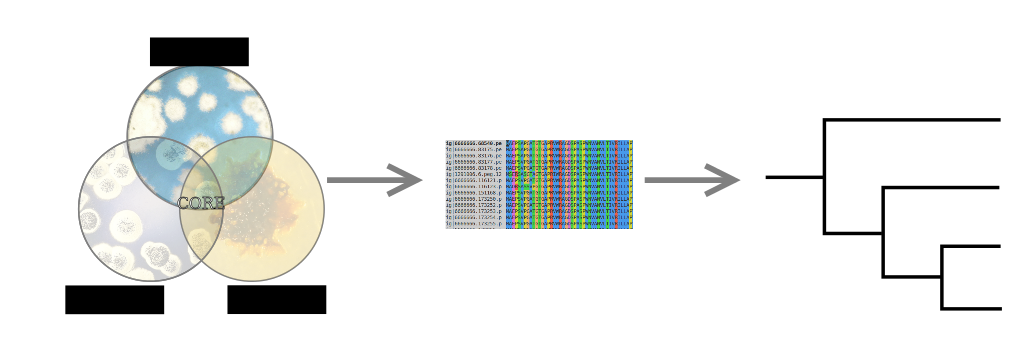
\includegraphics[angle = 0,scale = .42]{chapter1/coreWiki.png}
  \caption[Orthocore calcula el core de un linaje genómico para proveer una filogenia]{\footnotesize{Orthocore calcula las familias génicas comunes de un linaje genómico. Después de un proceso de filtrado, alineamiento y curación concatena estas familias y entrega una reconstrucción filogenética.}}
  \label{fig:Orthocore}
  \end{figure}
  
  El pangenoma es el contenido génico total de un linaje taxonómico. Las
  familias génicas de un pangenoma pueden clasificarse según sus patrones
  de presencia-ausencia en cada genoma del linaje. De acuerdo a esta
  clasificación los principales grupos de familias génicas en un pangenoma
  son el \emph{core}, el \emph{shell} y el \emph{cloud} (dispensable)
  genome. El \emph{core genome} es el conjunto de familias con presencia
  en todos los genomas del linaje. Por ejemplo, la secuencia de la
  subunidad 16s del gene rRNA, así como diversos genes ribosomales que
  suelen estar en el core de la gran mayoría de los linajes bacterianos.
  El \emph{shell genome} es el grupo de familias presentes en la mayoría
  de los genomas pero no en todos. En el \emph{shell} se ubican por
  ejemplo familias que estaban en el \emph{core genome} pero que algunas
  bacterias del linaje sufrieron una dinámica de pérdida (o ganancia)
  génica. Mientras que el \emph{cloud genome} o dispensable genome es
  aquel grupo de familias que sólo ocurre en unos cuantos genomas del
  linaje.
  
  La organización filogenética de un linaje genómico permite la
  observación de pérdida y ganancia de familias génicas en organismos
  cercanos. Si los organismos están desordenados es difícil apreciar la
  dinámica genómica de aparición-desaparición de miembros de una familia
  génica. Ordenar los genomas de un linaje facilita apreciar cambios en el
  número de copias de una familia. Esto es relevante en el marco de esta
  tesis ya que cambios en los perfiles de promiscuidad podrían estar
  relacionados a copias extras de organismos cercanos. Orthocore es un
  algoritmo que utiliza el core conservado de un linaje genómico para
  facilitar la organización filogenética de sus organismos
  \autoref{fig:Orthocore}
  
  \section{La distribución de la función metabólica de las familias del
  pangenoma depende de la variabilidad del linaje
  seleccionado.}\label{la-distribucion-de-la-funcion-metabolica-de-las-familias-del-pangenoma-depende-de-la-variabilidad-del-linaje-seleccionado.}
  
  El número de familias génicas presentes en el pangenoma, así como su
  distribución en el \emph{core}, \emph{shell} y \emph{dispensable genome}
  depende de la elección de los genomas y del linaje genómico. Para
  entender esto se puede pensar en un ejemplo extremo, consideremos una
  bacteria de 1000 familias de genes de la cual se obtienen secuencias de
  diez genomas de la misma cepa. Estas secuenciaciones deberían ser
  prácticamente idénticas y en ese caso el \emph{core genome} sería 1000
  familias, el \emph{shell} y el \emph{dispensable genome} serían cero. En
  este caso, todo el metabolismo, tanto el central como el especializado
  estarían conservados dentro del \emph{core genome}, ya que el
  \emph{shell} y el \emph{dispensable genome} se encuentran vacíos. Sin
  embargo, si variamos el linaje taxonómico, y ahora estudiamos el
  pangenoma de 10 especies distintas del género \emph{Streptomyces} ahora
  el core genome estará compuesto por aproximadamente un tercio de su
  tamaño promedio, y dentro del \emph{core genome} es donde se encontrarán
  muchos de las familias dedicadas al metabolismo central o conservado
  (por ejemplo, familias de la glicólisis o síntesis de aminoácidos). En
  cambio muchas de las familias dedicadas al metabolismo especializado y
  pertenecientes a clústers biosintéticos de productos naturales (BGCs)
  estarán en el \emph{dispensable genome} pues \emph{Streptomyces} es
  productor de una gran variedad de metabolitos especializados y cada
  especie suele tener su producto característico.
  
  \begin{figure}[h!tbp]
  \centering
  \includegraphics[angle = 0,scale = .75]{chapter1/Metabolismo-Pangenoma.png}
  \caption[El metabolismo en el Pangenoma]{\normalsize{El metabolismo en el Pangenoma}}
  \label{fig:El pangenoma de un conjunto de genomas de un linaje puede ser clasificado en varios grupos. En este ejemplo, en el lado izquierdo de la figura se observa en gris el genoma dispensable compuesto por familias génicas presentes sólo en un genoma. En dos tonos de morado observamos el shell genome, familias que están presentes en la mayoría de los genomas del linaje, en este en caso dos o tres genomas. Finalmente en rojo se muestra el core, aquellas familias presentes en todos los genomas del linaje. El core contiene tanto familias muy conservadas con una sola copia por genoma ( C ), como familias expandidas. Las familias marcadoras (M) pueden ser parte del core conservado o de las familias expandidas. Del lado derecho se muestra una representación del pangenoma para cualquier número de genomas. Familias de metabolismo conservado tenderán a estar concentradas entre el core y el shell genome, mientras que el metabolismo especializado tendrá más representantes en el dispensable que en el core genome. Sin embargo tanto el tipo de metabolismo como el tamaño del core, shell y dispensable pueden variar según la diversidad de los organismos seleccionados. }
  \end{figure}
  
  El \emph{core genome} de un linaje, además de tener familias conservadas
  y prácticamente presentes en todo el dominio Bacteria también puede
  contener familias marcadoras. Estos genes marcadores permiten realizar
  pruebas de diagnóstico para colonizaciones bacterianas. A las familias
  que están presentes en el \emph{core genome} de un linaje A, pero que
  están completamente ausentes de un linaje B se les llama marcadoras. Por
  ejemplo genes conservados en la especie \emph{Streptomyces coelicolor}
  pero no conservados en \emph{Streptomyces rimosus} son genes marcadores
  de \emph{Streptomyces coelicolor} respecto de \emph{Streptomyces
  rimosus}. Estos mismos marcadores tal vez no sean marcadores respecto de
  \emph{Streptomyces lividans}, a pesar de la cercanía taxonómica entre
  estos organismos. La presencia de genes marcadores en el core depende de
  ambos linajes, por lo que es importante contar con algoritmos que
  permitan automatizar su cálculo.
  
  El número de familias en el pangenoma, ya sea en el \emph{core, shell o
  dispensable} genome no sólo depende de la divergencia o proximidad
  taxonómica de los organismos del linaje seleccionado, también depende de
  lo variable que sea el contenido génico en los genomas del linaje. A
  esta característica se le conoce como apertura. Hay especies, por
  ejemplo algunos patógenos, cuyo pangenoma se encuentra sumamente cerrado
  en el sentido de que no importa cuántos genomas se agreguen, el número
  de familias parece converger y ser asintótico rápidamente a una cota
  superior. En cambio especies o géneros que viven en una gran diversidad
  de hábitats suelen tener un pangenoma abierto. Esto significa que cada
  vez que se agrega un nuevo genoma aparecen otras familias que no estaban
  en los genomas anteriores. En los linajes con pangenoma abierto el
  número de familias nuevas al agregar un genomas seguirá una tendencia
  creciente y no asintótica.
  
  Además de la apertura, existen otros intentos de cuantificar la
  diversidad génica de un linaje. Está por ejemplo la fluidez, definida
  como el promedio de familias únicas entre familias totales por pares de
  genomas. El pangenoma bacteriano total, es decir el total de familias
  génicas en el dominio Bacteria es considerado abierto.
  
  \begin{figure}[h!tbp]
  \centering
  \includegraphics[angle = 0,scale = .8]{chapter1/CoreMarcadores.png}
  \caption[Core y genes Marcadores]{\normalsize{Core y genes Marcadores}}
  \label{fig:El core genome puede contener familias con funciones en distintos grupos metabólicos así como diversidad en el número de copias. Arriba se muestra que en el core pueden coexistir familias tanto de copia única como con expansiones. Las familias con funciones en el metabolismo conservado suelen concentrarse en el core genome (rojas), pero también dependiendo de los organismos seleccionados pueden encontrarse ya sea familias enteras o algunas copias dedicadas al metabolismo especializado (azul). No de todas las copias se conocerá su función, algunas pueden tener un destino metabólico desconocido (gris) o bien ser predichas por algún algoritmo como parte del metabolismo especializado (cyan).  Abajo a la izquierda se comparan familias del core conservado con exactamente una copia por genoma contra familias del core expandido. Ambas pertenecen al core, pero en el core expandido hay dos genomas que tienen una copia extra en esta familia, unoa cyan y una gris, que podría dificultar la elección de los verdaderos ortólogos. A la derecha se ejemplifican familias de genes marcadores, útiles para identificar un linaje genómico. Tanto familias del core conservado como del core expandido pueden ser familias marcadores, siempre que exista al menos una copia de cada familia en el linaje 1 y ninguna copia en el linaje 2. Las familias dejan de ser marcadoras cuando el linaje dos contiene al menos una copia en algún genoma.}
  \end{figure}
  
  Finalmente la distribución de las funciones metabólicas encontrada en
  los subconjuntos del pangenoma ( \emph{core, shell y dispensable}
  genome) está relacionada a la proximidad filogenética de los organismos
  seleccionados en el estudio. Entre más diversos sean los organismos
  menos familias dedicadas exclusivamente a metabolismo especializado
  abundarán en el \emph{core/shell genome}. La diversidad provocará que lo
  único que tengan los genomas de estos organismos en común sean funciones
  conservadas por una amplia variedad de especies bacterianas. Ahora bien,
  muchas familias de metabolismo especializado provienen de reclutamientos
  de copias extra de familias de metabolismo conservado. Así pues aunque
  decrezca el número de familias con exclusividad en metabolismo
  especializado en el \emph{core y shell genome}, estos sunconjuntos del
  pangenoma aún pueden contener familias conservadas que tengan copias
  extra en proceso de reclutamiento para algún Cluster biosintético de
  genes (BGCs) de metabolismo especializado. Considerando las reflexiones
  anteriores, entre más diverso sea un linaje, más tenderá su \emph{core
  genome} a contener exclusivamente familias de metabolismo conservado
  mientras que su dispensable genome estará formado mayormente por
  familias de enzimas del metabolismo especializado.
  
  \section{El core conservado permite la reconstrucción de filogenias
  complicadas}\label{el-core-conservado-permite-la-reconstruccion-de-filogenias-complicadas}
  
  Orthocore es el desarrollo bioinformático que realicé para calcular las
  familias génicas más conservadas del \emph{core genome}. Dos genes son
  homólogos si poseen un ancestro común, entre los principales grupos de
  homólogos están ortólogos y parálogos. Los ortólogos provienen de
  eventos de especiación de un ancestro común mientras que los parálogos
  evolucionan por eventos de duplicación. Orthocore obtiene un subconjunto
  del \emph{core genome}: el \emph{core conservado}, es decir, familias de
  ortólogos presentes en todos los genomas del grupo y que además son
  libres de parálogos de difícil identificación. El \emph{core conservado}
  facilita la organización en árboles filogenéticos de organismos de un
  linaje genómico.
  
  La comparación de la variación molecular entre ortólogos ha sido
  utilizada para establecer relaciones filogenéticas entre organismos.
  Esta técnica ha dado lugar a grandes descubrimientos. Por ejemplo
  comparar la secuencia de la subunidad 16s del gene RNA ribosomal condujo
  a Woese al descubrimiento del dominio Archaea en 1977
  {[}\protect\hyperlink{ref-woese_phylogenetic_1977}{124}{]}. Un árbol de
  especies suele hacerse con secuencias de familias que pertenecen al core
  genome de un Dominio, por ejemplo las familias 16s o RpoB en los
  Dominios Bacteria y Archaea. Algunos autores realizan árboles multilocus
  para mejorar la resolución de árboles de especies realizados mediante la
  comparación de secuencias de 16s. Los genes seleccionados para los
  árboles multilocus deben estar en todos los organismos y no tener copias
  extra tan parecidas que puedan confundirse y entorpecer la
  reconstrucción filogenética, es decir, las familias seleccionadas deben
  ser parte del \emph{core conservado}. Orthocore automatiza la
  identificación de estas familias.
  
  Entre los factores importantes para establecer las relaciones
  filogenéticas diferenciando entre Archaea y Bacteria están los
  siguientes: 1) la presencia conservada de la subunidad de 16s en los
  tres dominios mencionados, y 2) la suficiente divergencia entre estas
  secuencias en los organismos de dichos dominios. Ahora bien, establecer
  relaciones filogenéticas entre Archaea y Bacteria es en cierto sentido
  más sencillo que establecerlas entre organismos pertenecientes al mismo
  género o inclusive a la misma especie. En ocasiones, como en el caso del
  género \emph{Streptomyces}, la secuencia de 16s por sí sola no posee la
  suficiente variación para resolver la filogenia
  {[}\protect\hyperlink{ref-labeda_phylogenetic_2017}{140}{]}. En
  \emph{Streptomyces} la variación entre estas secuencias suele ser menor
  al 1\%. Para resolver el problema de escasa variación en secuencias de
  16s se pueden concatenar las secuencias de otros ortólogos, siempre que
  estos aparezcan en todos los organismos que se estén estudiando, es
  decir, siempre que sean parte del core genómico.
  
  \section{El algoritmo de Orthocore}\label{el-algoritmo-de-orthocore}
  
  \begin{figure}[h!tbp]
  \centering
  \includegraphics[angle = 0,scale = .55]{chapter1/Best-n-directional.png}
  \caption[Best-n-directional hits]{\normalsize{Best-n-directional hits}}
  \label{fig:Orthocore utiliza los mejores hits n-direccionales para obtener grupos de ortólogos. Un hit es el mejor resultado de una secuencia en otro genoma. Un Bidireccional Best Hit es el mejor hit bidireccional, La secuencia 2 es el mejor hit de la secuencia 1 en el genoma 2 y recíprocamente, la secuencia 1 es el mejor hit de la secuencia 2 en el genoma 1. La existencia de una copia extra muy parecida a la secuencia 2 puede romper el BBH. Un mejor hit n-direccional debe ser BBH todos contra todos garantizando que estas secuencias están muy conservadas entre sí.}
  \end{figure}
  
  Los ortólogos suelen identificarse por similitud de secuencia, pero si
  se realiza la identificación manualmente también se suelen capturar
  parálogos que pueden confundir la elucidación de eventos de especiación.
  Orthocore automatizó la búsqueda de ortólogos y el filtrado de parálogos
  en genomas procariontes mediante la generalización de la definición del
  mejor hit bidireccional (BBH por sus siglas en inglés). Dos secuencias
  son BBH si cada una es el mejor hit de un algoritmo de distancia (BLAST
  usualmente) en el genoma de origen de la otra. Una primera
  generalización para obtener el set de ortólogos de una familia del core
  es definir un genoma de referencia y tomar los BBH respecto a ese
  genoma. En la práctica, esta definición da como resultado distintos
  resultados según el genoma de referencia, haciendo que algunos parálogos
  no sea filtrados.
  
  Para solventar esta dificultad se definió en Orthocore el concepto de
  mejores hits multidireccionales. Un conjunto de genes son mejores hits
  multidireccionales si todos entre sí son BBH por pares. Es decir si cada
  gen fuera un punto y ser mejor hit se expresara como una conexión con
  dirección todos los puntos estarían conectados por una flecha de ida y
  otra de regreso. Con este método se eliminó la dependencia de un genoma
  de referencia. Esta restricción también ocasiona que en grupos muy
  grandes por ejemplo más de 100 genomas de distintas especies, o muy
  diversos de distintos dominios, o muy fragmentados como con contigs de
  en promedio 3 Mbp, el core conservado puede quedar vacío.
  
  \subsection{Componentes técnicos de
  Orthocore}\label{componentes-tecnicos-de-orthocore}
  
  Orthocore es un tubería escrita en perl que incorpora los hits
  multidireccionales permitiendo obtener y usar el core conservado para
  realizar una reconstrucción filogenética mediante los siguientes pasos:
  
  -Obtiene el core conservado: los mejores n-direcional hits (blastp).\\
  -Alinea cada familia del core conservado (MUSCLE).\\
  -Cura automáticamente cada familia del core conservado (Gblocks).\\
  -Concatena las familias del core conservado formando una matriz de
  aminoácidos.\\
  -Realiza una reconstrucción filogenética de la matriz de aminoácidos
  (FastTree)\\
  -Provee las funciones del core conservado según la anotación funcional
  de RAST.
  
  Existen otros algoritmos como OrthoMCL, y fastOrtho que dividen
  pangenomas en clusters de familias de genes, get\_homologues y metaphor
  que obtienen el core y filtran buscando verdaderas relaciones de
  homología, y finalmente BPGA que hace reconstrucciones filogenéticas
  tanto según el core como según el pangenoma. Sin embargo Orthocore
  resolvió en su momento la necesidad específica de proporcionar una
  matriz concatenada de genes del core conservado lista para utilizarse en
  un árbol multilocus. Adicionalmente, como Orthocore fue diseñado para
  trabajar con la anotación de la plataforma RAST, también se obtiene la
  anotación funcional tanto de familias del core como del complemento.
  
  Orthocore incorpora todas las dependencias en un contenedor de docker
  disponible en \url{https://github.com/nselem/orthocore}. Además en este
  contenedor está un script que permite bajar genomas de NCBI masivamente
  y posteriormente anotarlos en RAST desde la terminal. Los protocolos de
  uso se encuentran al final de este capítulo.
  
  \subsection{Aplicaciones de Orthocore, identificación del core
  conservado y de familias de genes
  marcadores.}\label{aplicaciones-de-orthocore-identificacion-del-core-conservado-y-de-familias-de-genes-marcadores.}
  
  Cuatro aplicaciones de Orthocore serán presentadas en las siguientes
  secciones de este capítulo. En la primera aplicación el core conservado
  en \emph{Actinomycetales} permitió organizar filogenéticamente a este
  orden. Esta organización facilitó el entendimiento en cambios de
  promiscuidad de la familia enzimática PriA mediante la distinción de
  patrones de pérdida y ganancia de genes en las rutas de síntesis de
  histidina y triptófano. En la segunda aplicación cepas de
  \emph{Salmonella tifi} fueron ordenadas filogenéticamente. La tercera
  aplicación permitió realizar una reconstrucción filogenética del orden
  \emph{Nostocales} del phylum \emph{Cyanobacteria} y comparar así
  patrones de presencia y ausencia de clusters de genes biosintéticos.
  Finalmente, en organismos del microbioma del tomate orthocore de utilizó
  para identificar genes marcadores que permitieran distinguir cepas de
  \emph{Clavibacter Michiganensis} de otras especies de
  \emph{Micrococcales}.
  
  Perfiles de promiscuidad de PriA en el orden \emph{Actinomycetales} se
  relacionan con la especiación. Para mejorar el entendimiento de los
  cambios en promiscuidad enzimática de PriA, se necesitaba entender
  filogenéticamente al orden \emph{Actinomycetales}, un camino era obtener
  su core conservado. Orthocore fue diseñado para resolver este problema.
  Con el resultado de Orthocore se realizó un árbol de especies donde se
  observaron patrones de pérdida y ganancia de genes en la vecindad
  genómica del gen que codifica para PriA. Se encontró que hay clados de
  \emph{Actinomyces} donde los genes correspondientes a la síntesis de
  histidina no estaban en la vecindad genómica de PriA, y mediante la
  realización de cinéticas enzimáticas se comprobó que la actividad de
  catalizar la reacción correspondiente a HisA estaba perdida en estos
  organismos. A estas enzimas se les llamó subTrpF ya que sólo poseían la
  capacidad de catalizar la reacción correspondiente a la familia TrpF.
  Del mismo modo existían clados que perdieron los genes de síntesis de
  triptófano en la vecindad de PriA y estas enzimas se subfuncionalizaron
  a la familia subHisA. De estos datos se observa que en estos organismos
  la especiación coincidió con el cambio de promiscuidad en la familia
  PriA, acorde a la pérdida y ganancia de genes vecinos. La promiscuidad
  puede co-ocurrir con variaciones en el contexto genómico, pudiendo estos
  cambios ser una marca para sugerir cambio funcional en una familia.
  
  \subsection{\texorpdfstring{Genes de islas de patogenicidad de
  \emph{Salmonella} en México están conservados en la mayoría de los
  genomas.}{Genes de islas de patogenicidad de Salmonella en México están conservados en la mayoría de los genomas.}}\label{genes-de-islas-de-patogenicidad-de-salmonella-en-mexico-estan-conservados-en-la-mayoria-de-los-genomas.}
  
  Para estudiar la diversidad de \emph{Salmonella} presente en alimentos
  en México, primero se ensamblaron y anotaron genomas secuenciados para
  el trabajo ``distribución de los genes de la toxina VirB/D4 en plásmidos
  de bovino asociados a Salmonella no tifoidal''. Los genomas fueron
  ensamblados en Patrick y se desarrolló myRAST, una tubería previa a
  Orthocore para la anotación automática de genomas ensamblados en RAST.
  El protocolo de myRAST puede encontrarse al final de este capítulo.
  
  Orthocore fue usado aquí para reconstruir filogenias de
  \emph{Salmonella} y además fue integrado como parte de CORASON, el cual
  se reporta en el Capítulo 3, es el algoritmo que sirve para visualizar
  variantes de clusters organizados filogenéticamente. Los clusters de
  genes pueden ser biosintéticos, islas de patogenicidad, operones o
  cualquier región parcialmente sinténica de un genoma bacteriano centrada
  en un gen. En este caso se observó una alta conservación de toxinas
  tifoidales en islas de patogenicidad de Salmonella. Éstas fueron
  identificadas en 76\% de las cepas analizadas y posteriormente
  visualizadas mediante CORASON.
  
  \subsection{Nostoc provenientes del metagenoma de cícadas se agrupan
  Cyanobacteria}\label{nostoc-provenientes-del-metagenoma-de-cicadas-se-agrupan-cyanobacteria}
  
  \begin{figure}[h!tbp]
  \centering
  \includegraphics[angle = 0,scale = .45]{chapter1/Nostoc.png}
  \caption[Arbol de Nostoc derivado de la selección  de genes del core conservado]{\normalsize{Arbol de Nostoc derivado de la selección  de genes del core conservado}}
  \label{fig:Reconstrucción de 76 taxa provenientes de 7 órdenes de Cyanobacteria. La matriz final incluyó 45,475 aminoácidos curados de 198 familias de proteínas pertenecientes al core conservado. A la derecha se muestra un zoom del orden Nostocales que incluye bacterias simbiontes de cícadas. Metadatos como el tamaño de genoma, contenido de GC y hábitat de origen muestran una posible tendencia de incremento de tamaño en los genomas provenientes del microbioma de plantas.}
  \end{figure}
  
  Las Cyanobacterias son un phylum de bacterias que se han adaptado a
  diversos ambientes. Aunque muchas de ellas son marinas algunas
  Cyanobacterias viven como simbiontes de plantas. En particular las
  cícadas han desarrollado un tipo especial de raíz donde se sabe que vive
  como simbionte el género \emph{Nostoc}. La presencia de \emph{Nostoc} en
  la raíz coraloide de las cícadas es fácilmente distinguible por la
  formación de un anillo verde conocido como anillo cyanobacterial. En la
  figura se muestra la filogenia de 76 Cyanobacterias de 7 órdenes
  distintos construida con 198 proteínas del core conservado obtenidas por
  Orthocore. En esta reconstrucción se puede observar que los
  \emph{Nostoc} asociados a plantas tienden a agruparse en la filogenia.
  
  \subsection{Identificación de genes marcadores de Clavibacter
  michiganensis}\label{identificacion-de-genes-marcadores-de-clavibacter-michiganensis}
  
  \emph{Micrococcales} es un orden de Actinobacteria que contiene a
  \emph{Clavibacter}, \emph{Micrococcus} y \emph{Microbacterium}, entre
  otros microorganismos. El género \emph{Clavibacter} comprende especies
  que pueden causar enfermedades en diversas plantas. En particular la
  especie \emph{Clavibacter michiganensis} es una bacteria causante de la
  enfermedad del cáncer del tomate. \emph{Clavibacter michiganensis} ha
  sido frecuentemente aislada en compañía de otros \emph{Micrococcales}
  morfológicamente parecidos. La distinción entre microorganismos debida a
  la comparación de la secuencia de 16s no era suficiente para distinguir
  entre \emph{Micrococales} del microbioma del tomate, por lo que una
  prueba de diagnóstico se hacía necesaria. Se habían utilizado como
  marcadores genes como \emph{tomA}, \emph{ppaC} y \emph{celA} entre
  otros, sin embargo estas elecciones en ocasiones resultaban en falsos
  positivos según árboles de especies de 16s, por lo que nuevos marcadores
  eran necesarios.
  
  \begin{figure}[h!tbp]
  \centering
  \includegraphics[angle = 0,scale = .5]{chapter1/Marcadores-Clavibacter.png}
  \caption[Marcadores-Clavibacter]{\normalsize{Marcadores-Clavibacter}}
  \label{fig: Los marcadores moleculares previos a este trabajo no permitían diferenciar correctamente a Clavibacter michiganensis respecto al microbioma del tomate en invernaderos mexicanos. Arriba a la izquierda se muestran los antiguos marcadores tomA, ppaC, ppaH, pelA1, celA. Abajo organismos pertenecientes al microbioma del tomate. Orthocore obtuvo el core conservado de siete cepas de Cmm patógenas, y este core se utilizó para definir nuevos marcadores. Aunque tomA pertenecía al core conservado de Cmm, estaba también incluido en el pangenoma del microbioma del tomate. Después de calcular la intersección core conservado de Cmm y pangenoma del microbioma se obtuvieron entre las familias marcadoras genes clv parte del cluster biosintético de clavidicina (michiganina).}
  \end{figure}
  
  Al analizar en RAST genomas de \emph{Microbacterium} y
  \emph{Micrococcus} aislados de tomate se encontró que en efecto,
  \emph{tomA} y los otros marcadores propuestos previamente no eran
  exclusivos de \emph{Clavibacter michiganensis} ( \emph{Cmm} ). Al
  utilizar Orthocore en siete genomas de \emph{Cmm} encontramos que varios
  genes del cluster biosintético de michiganina (BGC0000528 en MIBiG)
  codificado por los genes \emph{clvAFGLKM} pertenecían al core
  conservado, pero que al agregar los genomas no Cmm del resto del
  microbioma del tomate los genes \emph{clv} se pierden. El descubrimiento
  de que \emph{clv} pertenecía al core de \emph{Cmm} se realizó con
  secuencias de genomas muy fragmentados, en la figura se muestran las
  cepas originales que fueron analizadas.
  
  \begin{figure}[h!tbp]
  \centering
  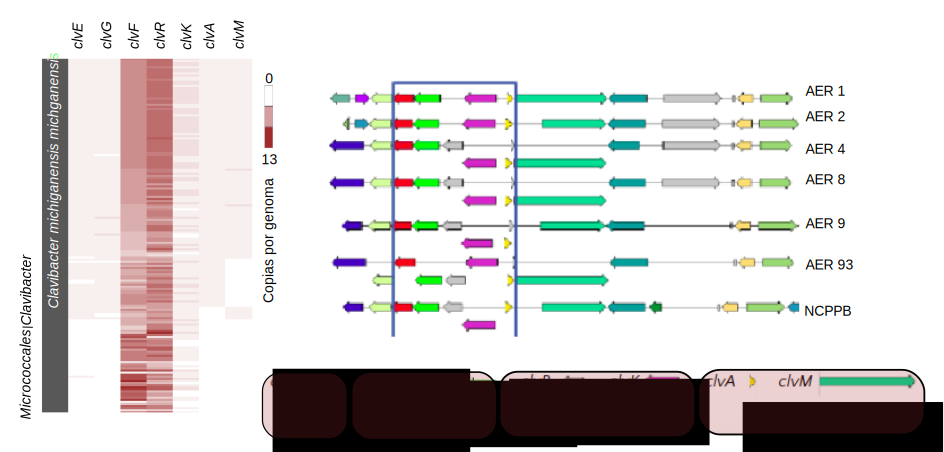
\includegraphics[angle = 0,scale = .6]{chapter1/clv.png}
  \caption[ clv BGC]{\normalsize{ clv BGC}}
  \label{fig:Marcadores-Clavibacter}
  \end{figure}
  
  Esta observación se corroboró con más genomas, en este caso se muestran
  como ejemplo 10 genomas de bacterias del microbioma del tomate, entre
  ellas siete \emph{Clavibacter}, seis de tomates de invernadero y uno
  \emph{Clavibacter} proveniente de tomate silvestre, \emph{Clavibacter}
  RA1B que fue reportado en la tesis de maestría de Yanez. Con Orthocore
  vemos que el tamaño del core decrece al ir agregando genomas de
  \emph{Clavibacter} y decrece aún más rápido al agregar los genomas de
  \emph{Micrococcus} y \emph{Microbacterium} La reconstrucción
  filogenetica de este microbioma, ubica a \emph{Clavibacter} RA1B cerca
  de los otros \emph{Cmm} pero no en un clado junto con ellos. Una
  búsqueda por blast revela que los genes marcadores de \emph{Cmm}:
  \emph{clvF}, \emph{clvR} son también marcadores de \emph{Clavibacter}
  RA1B pero no así \emph{clvA} y \emph{clvG} que solamente están presentes
  en el core de \emph{Cmm}. Sin embargo \emph{clvF} y \emph{clvR} no están
  en el contexto del cluster de michiganina en RA1B y su similitud de
  secuencia es menor que la que se observa entre los otros \emph{Cmm}.
  
  De hecho al considerar más genomas dentro del microbioma del tomate, la
  familia \emph{clvF} no solo no está en el core conservado de
  \emph{Microbacterium} y \emph{Micrococcus}, sino que no está presente en
  ningún otro genoma distinto a \emph{Clavibacter}. Con distintos niveles
  de conservación de secuencia los genes \emph{clv} son un buen marcador
  para distinguir \emph{Cmm} de otras especies, por esta razón estos genes
  aún se encuentran en uso como genes marcadores de \emph{Cmm}. Esta misma
  conclusión se reporta en el trabajo de yasuhara, su observación de que
  las familias \emph{clvA, clvF} y \emph{clvG} son exclusivas de
  \emph{Cmm} es independiente de la nuestra, fue hecha sin análisis
  genómicos y basada en evidencia experimental
  {[}\protect\hyperlink{ref-yasuhara-bell_genes_2014}{141}{]}. Este
  descubrimiento ha permitido bajar los costos de identificación de
  Clavibacter, ya que ahora en lugar de enviar a secuenciar el genoma es
  suficiente identificar por PCR \emph{clvF} en conjunto con otro
  marcadores.
  
  Con Orthocore además de obtener los genes marcadores podemos obtener
  también la matriz del core conservado para realizar la reconstrucción
  filogenética de especies cercanas de \emph{Clavibacter}. Debido a que es
  importante para los agricultores conocer de dónde provienen las
  bacterias que infectan al tomate, una de las líneas de investigación del
  laboratorio de evolución de la diversidad metabólica, es la organización
  taxonómica de cepas de \emph{Cmm} y de otras bacterias del microbioma de
  tomate. Por este motivo se tienen unos doscientos genomas privados y se
  esperan más a futuro. Orthocore colabora con esta investigación
  proporcionando matrices multilocus que pueden diferenciar entre
  \emph{Clavibacter} de la misma o de diferente especie.
  
  \begin{figure}[h!tbp]
  \centering
  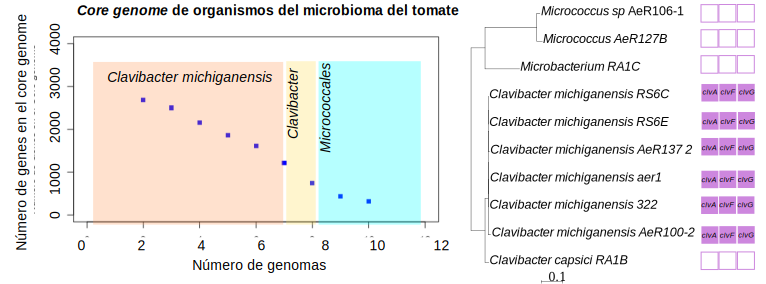
\includegraphics[angle = 0,scale = .5]{chapter1/CoreGenomeMicrobioma.png}
  \caption[ X X Evomining]{\normalsize{ X X Evomining}}
  \label{fig:Marcadores-Clavibacter EvoMining}
  \end{figure}
  
  Debido al intercambio génico por transferencia horizontal en las
  bacterias, es posible que los genes marcadores actuales alguna vez
  aparezcan en otros organismos. También las bacterias pierden
  continuamente genes, por lo que es posible que algún gen marcador de Cmm
  se pierda en una cierta cepa. Esto hace que la definición de estar
  presentes en el core del grupo de interés y ausentes totalmente de cada
  uno de los genomas de otro linaje ya no funcione completamente. Sin
  embargo, en estas dos situaciones presentadas, ganancia de genes
  marcadores de organismos externos al linaje original o pérdida de genes
  marcadores en algunas cepas, se sigue cumpliendo que los ex genes
  marcadores, estarán presentes en la mayoría de los organismos del linaje
  de interés y ausentes de la mayoría de los organismos del linaje
  externo. Por ello, se pensó que está definición de genes marcadores se
  podía generalizar clasificando a grupos de genes ortólogos acorde a sus
  porcentajes de ocurrencia. Esta idea se desarrolló en la herramienta
  clavisual, explicada en la siguiente sección.
  
  \section{Clavisual: Identificación de genes marcadores a un cierto
  porcentaje de grupos
  seleccionados}\label{clavisual-identificacion-de-genes-marcadores-a-un-cierto-porcentaje-de-grupos-seleccionados}
  
  La idea de que Orthocore puede ser usado para obtener los genes
  marcadores de un grupo taxonómico frente a otro fue generalizada en el
  backend del software Clavisual. Ya se ha explicado previamente que el
  core puede salir vacío por diversas razones, entre ellas baja calidad de
  los genomas, o que éstos provengan de organismos muy divergentes,
  verdaderas razones biológicas como dinámica génica o un core no
  convergente. Así pues, es posible que si sólo se utiliza el core no se
  obtengan marcadores. Pero el core puede relajarse de varias maneras una
  de ellas es el Pseudocore, donde en lugar de multidireccional hits se
  toman BBH a un genoma de referencia. Otra forma es establecer un
  porcentaje de presencia /ausencia de interés.
  
  El pseudocore consiste en \_\_\_\_\_\_\_\_ y la metodología está
  depositada en github en el repositorio\_\_\_\_\_\_\_\_\_. El blast fue
  optimizado cambiando hacer un blast todos contra todos por archivos
  genómicos individuales genomai\_vs\_genomaj.blast que luego son
  concatenandos según se necesiten.
  
  Los porcentajes de genomas son diferentes porque al no bastar los best
  bidireccional hits conservados, todo el pangenoma es decir todos los
  genes contenidos en los genomas del grupo de interés necesitan ser
  clasificados por familias, para de ahi obtener las familias que tienen
  presencia en un porcentaje \%p y ausencia en un porcentaje a\% del grupo
  externo. Estos perfiles fueron desarrollados para Clavisual utilizando
  FasthOrtho para clasificar las familias y de ahi obtener los grupos. Con
  ellos se consiguieron marcadores para Kurtobacterium.
  
  Finalmente Clavisual despliega un árbol realizado con el Pseudocore
  respecto a un conjunto de genes de Cmm NCPP previamente seleccionados.
  En este árbol clavisual permite la visualización de metadatos, como año,
  género de la bacteria, estado de salud de la planta e invernadero donde
  fue aislada.
  
  \begin{figure}[h!tbp]
  \centering
  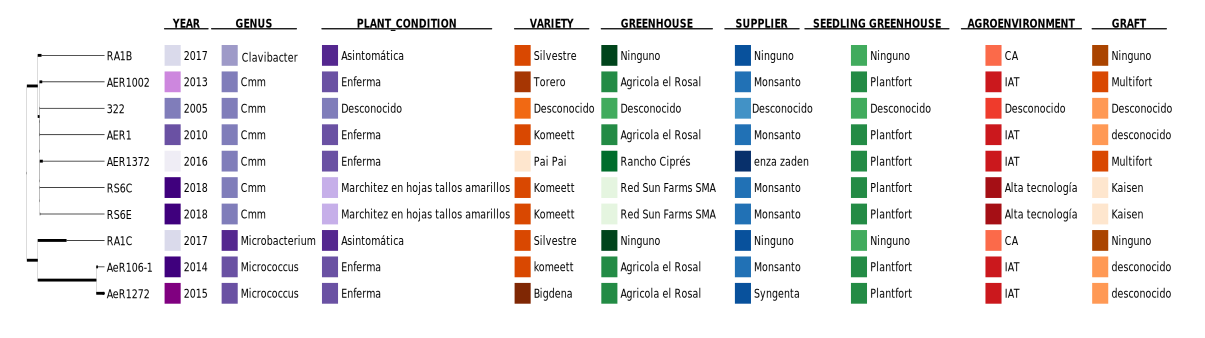
\includegraphics[angle = 0,scale = .4]{chapter1/Clavisual.png}
  \caption[ X X]{\normalsize{ X X}}
  \label{fig:Clavisual}
  \end{figure}
  
  \subsection{El pangenoma de Clavibacter Michiganensis es
  abierto}\label{el-pangenoma-de-clavibacter-michiganensis-es-abierto}
  
  Después de desarrollar métodos de identificación de genes marcadores y
  generalizarlo a obtener grupos con patrones de presencia/ausencia
  definidos por el usuario, quedaba por responder la pregunta cómo es el
  pangenoma de \emph{Cmm}. Algunos autores consideran que el pangenoma de
  patógenos es reducido porque sus genomas suelen sufrir proceso de
  reducción de tamaño débido a la pérdida de genes. Como \emph{Cmm} es un
  patógeno de planta quedaba por investigar cómo es su pangenoma. ¿Es
  posible saturar el contenido génico de \emph{Cmm} con sólo secuenciar
  más genomas?. Aunque actualmente existen ya herramientas web para el
  análisis de pangenoma, en su momento se utillizó el software bpga que se
  corre desde la terminal. Para facilitar su instalación se desarrolló un
  docker que se describe más tarde en este capítulo en la sección de las
  descripciones técnicas. Como ejemplo de su funcionamiento, se analizó el
  pangenoma de los mismos diez genomas del pangenoma del tomate utilizados
  en la visualización de clavisual.
  
  \begin{figure}[h!tbp]
  \centering
  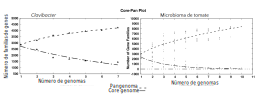
\includegraphics[angle = 0,scale = .5]{chapter1/bpga-pangenoma.png}
  \caption[ X X]{\normalsize{ X X}}
  \label{fig:bpga-pangenoma}
  \end{figure}
  
  Tomando otros siete clavibacters, utilizando OrthoVenn tenemos la misma
  observación, el número de familias de genes agregadas al adicionar
  genomas, es después de siete genomas casi tan grande como su core.
  
  \begin{figure}[h!tbp]
  \centering
  \includegraphics[angle = 0,scale = .5]{chapter1/Venn_chart.pdf}
  \caption[ X X]{\normalsize{ X X}}
  \label{fig:Venn Chart}
  \end{figure}
  
  \section{Relación entre genes marcadores, Orthocores y la promiscuidad
  enzimática.}\label{relacion-entre-genes-marcadores-orthocores-y-la-promiscuidad-enzimatica.}
  
  Finalmente, al aplicar Orthocore para detectar genes marcadores se
  vuelve indirectamente reclutamientos al metabolismo especializado, cómo,
  pues porque dentro de los marcadores hay productos naturales como,
  PENDIENTE VER RESULTADOS RETRO-EVOMINING la clavidicina (michiganina).
  Ahí vemos que clvABCDEF participan en metabolismo secundario, las
  enzimas de metabolismo central de este cluster pueden presentar cierta
  promiscuidad.
  
  \section{Protocolos para usar Orthocore, myRAST, fastOrtho,
  Clavigenomics, y
  BPGA}\label{protocolos-para-usar-orthocore-myrast-fastortho-clavigenomics-y-bpga}
  
  Anotación genómica con el docker myRAST
  
  Esta es una distribución de myRAST en un contenedor de docker. Para
  usarla se necesita una cuenta del anotador genómico RAST. el docker
  myRAST permite hacer anotación genómica y funcional masiva mediante el
  uso de la terminal en el anotador RAST. Después de anotar los resultados
  pueden descargarse y procesarse en una terminal
  
  Descargar myrast docker distribution
  
  Una vez con docker instalado en la computadora, se hace pull al docker
  myrast.
  
  docker pull nselem/myrast\\
  Abrir myRast en la terminal
  
  docker run -i -t -v \$(pwd):/home nselem/myrast /bin/bash
  
  Usar myRast
  
  -Ejemplo subir un archivo fasta
  
  svr\_submit\_RAST\_job -user -passwd -fasta -domain Bacteria -bioname
  ``Organism name'' -genetic\_code 11 -gene\_caller rast
  
  -Para bajar un archivo de anotación genómica funcional:
  
  svr\_retrieve\_RAST\_job table\_txt \textgreater{} \$ID.txt
  
  Una lista completa de archivos puede ser procesada usando bash. Por
  ejemplo para bajar una lista de archivos de RAST se deben guardar los
  identificadores de RAST en una columna de un archivo, (Rast\_ID en este
  ejemplo) y usar un while para obtenerlos:
  
  En este caso la variable ``line'' contendrá el identificador RAST Id, y
  cada archivo fasta de aminácidos podrá ser obtenido mediante su
  identificador de RASTy será guardado en el archivo ``\$line.faa''
  
  cut -f1 Rast\_ID \textbar{} while read line; do svr\_retrieve\_RAST\_job
  \$line amino\_acid \textgreater{} \$line.faa ; done\\
  Formatos de RAST para descargar archivos
  
  Puedes cambiar el formato table\_txt por el que tú necesites.
  
  Pie de tabla
  
  \textbar{}Atributo \textbar{}Descripción \textbar{}\\
  \textbar{}genbank \textbar{}GenBank (con funciones y enriquecimiento de
  SEED) \textbar{}\\
  \textbar{}genbank\_stripped\textbar{}Genbank con EC-numbers removidos de
  las funciones\textbar{}\\
  \textbar{}embl \textbar{}EMBL (con funciones y enriquecimiento de SEED)
  \textbar{}\\
  \textbar{}embl\_stripped \textbar{}EMBL con EC-numbers removidos de las
  funciones\textbar{}\\
  \textbar{}gff3 \textbar{}GFF3\textbar{}\\
  \textbar{}gff3\_stripped \textbar{}GFF3 con EC-numbers removidos de las
  funciones\textbar{}\\
  \textbar{}gtf \textbar{}GTF\textbar{}\\
  \textbar{}gtf\_stripped\textbar{} GTF con EC-numbers removidos de las
  funciones\textbar{}\\
  \textbar{}rast\_tarball \textbar{} Archivo comprimido (gzipped) con todo
  el directorio de las anotaciones de RAST sobre el genoma\textbar{}\\
  \textbar{}nucleic\_acid\textbar{} Fasta de DNA de genes\textbar{}\\
  \textbar{}amino\_acid \textbar{}Fasta de DNA de aminoácidos\textbar{}\\
  \textbar{}table\_txt\textbar{}Gene data in tab-separated
  format\textbar{}\\
  \textbar{}table\_xls\textbar{}\textbar{}
  
  \section{ORthocore}\label{orthocore}
  
  El umbral de e-value de Orthocore es por default 1e-6. Todas las
  secuencias son alineadas usando MUSCLE v3.8.31 con los parámetros
  default y curadas utilizando Gblocks con 5 posiciones como longitud
  mínima del bloque, 10 como máximo número de posiciones contiguas no
  conservadas y sólo considerando posiciones con gaps menores que el 50\%
  de las secuencias en el alineamiento final. Después de esta curación las
  secuencias son concatenadas en una matriz final.
  \texttt{\{r\ chapter2,\ child\ =\ \textquotesingle{}chap2.Rmd\textquotesingle{}\}}
  \texttt{\{r\ chapter3,\ child\ =\ \textquotesingle{}chap3.Rmd\textquotesingle{}\}}
  
  \texttt{\{r\ chapter4,\ child\ =\ \textquotesingle{}chap4.Rmd\textquotesingle{}\}}
  
  \chapter*{Conclusion}\label{conclusion}
  \addcontentsline{toc}{chapter}{Conclusion}
  
  \setcounter{chapter}{4} \setcounter{section}{0}
  
  Idea de Rosario -ver dell cluster de saxitoxin cuantos pasos se
  necesitron para llegar ahi.\\
  -A donde se iria el resultado de abrir el GMP\\
  -Otra vez, que Actinos tienen FolE
  
  \section{Discusion}\label{discusion}
  
  Finalmente, una pregunta abierta es aún dada una enzima promiscua es la
  población promiscua, y son sólo unos confórmeros o todas y cada una de
  las enzimas son promiscuas
  
  If we don't want Conclusion to have a chapter number next to it, we can
  add the \texttt{\{.unnumbered\}} attribute. This has an unintended
  consequence of the sections being labeled as 3.6 for example though
  instead of 4.1. The \LaTeX~commands immediately following the Conclusion
  declaration get things back on track.
  
  \subsubsection{More info}\label{more-info}
  
  And here's some other random info: the first paragraph after a chapter
  title or section head \emph{shouldn't be} indented, because indents are
  to tell the reader that you're starting a new paragraph. Since that's
  obvious after a chapter or section title, proper typesetting doesn't add
  an indent there.
  
  \appendix
  
  \chapter{The First Appendix}\label{the-first-appendix}
  
  This first appendix includes all of the R chunks of code that were
  hidden throughout the document (using the \texttt{include\ =\ FALSE}
  chunk tag) to help with readibility and/or setup.
  
  \subsubsection{In the main Rmd file:}\label{in-the-main-rmd-file}
  
  \begin{Shaded}
  \begin{Highlighting}[]
  \CommentTok{# This chunk ensures that the reedtemplates package is}
  \CommentTok{# installed and loaded. This reedtemplates package includes}
  \CommentTok{# the template files for the thesis and also two functions}
  \CommentTok{# used for labeling and referencing}
  \NormalTok{if(!}\KeywordTok{require}\NormalTok{(devtools))}
    \KeywordTok{install.packages}\NormalTok{(}\StringTok{"devtools"}\NormalTok{, }\DataTypeTok{repos =} \StringTok{"http://cran.rstudio.com"}\NormalTok{)}
  \NormalTok{if(!}\KeywordTok{require}\NormalTok{(reedtemplates))\{}
    \KeywordTok{library}\NormalTok{(devtools)}
    \NormalTok{devtools::}\KeywordTok{install_github}\NormalTok{(}\StringTok{"ismayc/reedtemplates"}\NormalTok{)}
  \NormalTok{\}}
  \KeywordTok{library}\NormalTok{(reedtemplates)}
  \end{Highlighting}
  \end{Shaded}
  
  \subsubsection{\texorpdfstring{In
  \protect\hyperlink{ref_labels}{}:}{In :}}\label{in}
  
  \begin{Shaded}
  \begin{Highlighting}[]
  \CommentTok{# This chunk ensures that the reedtemplates package is}
  \CommentTok{# installed and loaded. This reedtemplates package includes}
  \CommentTok{# the template files for the thesis and also two functions}
  \CommentTok{# used for labeling and referencing}
  \NormalTok{if(!}\KeywordTok{require}\NormalTok{(devtools))}
    \KeywordTok{install.packages}\NormalTok{(}\StringTok{"devtools"}\NormalTok{, }\DataTypeTok{repos =} \StringTok{"http://cran.rstudio.com"}\NormalTok{)}
  \NormalTok{if(!}\KeywordTok{require}\NormalTok{(plyr))}
      \KeywordTok{install.packages}\NormalTok{(}\StringTok{"plyr"}\NormalTok{, }\DataTypeTok{repos =} \StringTok{"http://cran.rstudio.com"}\NormalTok{) ## this shoul always go before dplyr}
  \NormalTok{if(!}\KeywordTok{require}\NormalTok{(dplyr))}
      \KeywordTok{install.packages}\NormalTok{(}\StringTok{"dplyr"}\NormalTok{, }\DataTypeTok{repos =} \StringTok{"http://cran.rstudio.com"}\NormalTok{)}
  \NormalTok{if(!}\KeywordTok{require}\NormalTok{(ggplot2))}
      \KeywordTok{install.packages}\NormalTok{(}\StringTok{"ggplot2"}\NormalTok{, }\DataTypeTok{repos =} \StringTok{"http://cran.rstudio.com"}\NormalTok{)}
  \NormalTok{if(!}\KeywordTok{require}\NormalTok{(reedtemplates))\{}
    \KeywordTok{library}\NormalTok{(devtools)}
    \NormalTok{devtools::}\KeywordTok{install_github}\NormalTok{(}\StringTok{"ismayc/reedtemplates"}\NormalTok{)}
    \NormalTok{\}}
  \KeywordTok{library}\NormalTok{(reedtemplates)}
  \end{Highlighting}
  \end{Shaded}
  
  \chapter{The Second Appendix, Open source code on this
  document}\label{the-second-appendix-open-source-code-on-this-document}
  
  \section{R markdown}\label{r-markdown}
  
  Thanks to Rmakdown Thesis\\
  Apendix one Useful docker commands\\
  -Create a new repository\\
  \texttt{docker\ build\ .\ -t\ evomining}\\
  \texttt{docker\ push\ nselemevomining}
  
  \section{Docker}\label{docker}
  
  Restart docker and free all ports\\
  \texttt{sudo\ service\ docker\ restart}
  
  list containers\\
  \texttt{docker\ ps\ -a}
  
  ssh or bash into a running docker container\\
  \texttt{sudo\ docker\ exec\ -i\ -t\ romantic\_brahmagupta\ /bin/bash}
  \texttt{docker\ exec\ -it\ \textless{}mycontainer\textgreater{}\ bash}
  
  Stop all containers\\
  \texttt{docker\ rm\ \$(docker\ ps\ -a\ -q)}
  
  Remove stopped containers\\
  \texttt{docker\ rm\ \$(docker\ ps\ -q\ -f\ status=exited)}
  
  Remove all images\\
  \texttt{docker\ rmi\ \$(docker\ images\ -q)}
  
  uninstall docker from ubuntu (Fresh start)\\
  \texttt{sudo\ apt-get\ purge\ docker-engine}\\
  \texttt{sudo\ apt-get\ autoremove\ -\/-purge\ docker-engine}\\
  \texttt{rm\ -rf\ /var/lib/docker} \# This deletes all images,
  containers, and volumes
  
  Run Evomining container using nselem/newevomining image\\
  \texttt{docker\ run\ -i\ -t\ -v\ /home/nelly/GIT/EvoMining/:/var/www/html/EvoMining/exchange\ -p\ 80:80\ nselem/newevomining\ /bin/bash}
  
  Start evomining inside this container\\
  \texttt{perl\ startevomining}
  
  Vizualice a tree\\
  \texttt{http://10.10.100.234/EvoMining/cgi-bin/color\_tree.pl?9\&\&/var/www/html/EvoMining/exchange/CyanosBBH\_MiBIG\_DB.faa\_CYANOS}
  file 9.new must be on folder volume CyanosBBH\_MiBIG\_DB.faa\_CYANOS
  
  Find a perl module\\
  \texttt{perl\ -MList::Util\ -e\textquotesingle{}print\ \$\_\ .\ "\ =\textgreater{}\ "\ .\ \$INC\{\$\_\}\ .\ "\textbackslash{}n"\ for\ keys\ \%INC\textquotesingle{}}
  EvoMining notes\\
  Gblocks only runs inside folder /var/www/html/EvoMining
  
  \section{Git}\label{git}
  
  \texttt{git\ add\ -\/-all}\\
  \texttt{git\ commit\ -m\ "Some\ message"}\\
  \texttt{git\ push\ -u\ origin\ master}\\
  \texttt{git\ clone}
  
  \section{Connect GitHub and
  DockerHub}\label{connect-github-and-dockerhub}
  
  automated builds The Dockerfile is available to anyone with access to
  your Docker Hub repository. Your repository is kept up-to-date with code
  changes automatically.
  
  \section{Additional resources}\label{additional-resources}
  
  \begin{itemize}
  \item
    \emph{Markdown} Cheatsheet -
    \url{https://github.com/adam-p/markdown-here/wiki/Markdown-Cheatsheet}
  \item
    \emph{R Markdown} Reference Guide -
    \url{https://www.rstudio.com/wp-content/uploads/2015/03/rmarkdown-reference.pdf}
  \item
    Introduction to \texttt{dplyr} -
    \url{https://cran.rstudio.com/web/packages/dplyr/vignettes/introduction.html}
  \item
    \texttt{ggplot2} Documentation -
    \url{http://docs.ggplot2.org/current/}
  \end{itemize}
  
  Docker antiSMASH run\_antismash /.gbk \textasciitilde{}/as\_results
  --knownclusterblast --inclusive --cf\_threshold 0.7
  
  \chapter{The third Appendix, Other contributions during my
  phd}\label{the-third-appendix-other-contributions-during-my-phd}
  
  \section{Accepted}\label{accepted}
  
  -Evomining identifies Arsenolipids biosynthetic cluster
  
  \section{Submitted}\label{submitted}
  
  \begin{itemize}
  \tightlist
  \item
    Siderophore micrococcus cluster identified by CORASON\\
  \item
    CORASON find genomes that owns cluster from cyanobacterial
    metagenome\\
  \item
    Streptomyces central pathways expanssions
  \end{itemize}
  
  \section{On preparation}\label{on-preparation}
  
  \begin{itemize}
  \tightlist
  \item
    PriA non Darwinian trayectories\\
    poner figura James unidades docking
  \end{itemize}
  
  \backmatter
  
  \chapter{References}\label{references}
  
  \noindent
  
  \setlength{\parindent}{-0.20in} \setlength{\leftskip}{0.20in}
  \setlength{\parskip}{8pt}
  
  \hypertarget{refs}{}
  \hypertarget{ref-khersonsky_enzyme_2010}{}
  1. Khersonsky O, Tawfik DS. Enzyme promiscuity: A mechanistic and
  evolutionary perspective. Annual Review of Biochemistry.
  2010;79:471--505.
  
  \hypertarget{ref-copley_enzymes_2003}{}
  2. Copley SD. Enzymes with extra talents: Moonlighting functions and
  catalytic promiscuity. Current Opinion in Chemical Biology
  {[}Internet{]}. 2003 Apr {[}cited 2017 Feb 8{]};7(2):265--72. Available
  from:
  \url{https://www.sciencedirect.com/science/article/pii/S1367593103000322}
  
  \hypertarget{ref-hult_enzyme_2007}{}
  3. Hult K, Berglund P. Enzyme promiscuity: Mechanism and applications.
  Trends in Biotechnology {[}Internet{]}. 2007 May {[}cited 2017 Feb
  8{]};25(5):231--8. Available from:
  \url{https://www.sciencedirect.com/science/article/pii/S016777990700073X}
  
  \hypertarget{ref-obrien_catalytic_1999}{}
  4. O'Brien PJ, Herschlag D. Catalytic promiscuity and the evolution of
  new enzymatic activities. Chemistry \& Biology {[}Internet{]}. 1999 Apr
  {[}cited 2017 Feb 9{]};6(4):R91--R105. Available from:
  \url{http://www.sciencedirect.com/science/article/pii/S1074552199800337}
  
  \hypertarget{ref-baronagomez_occurrence_2003}{}
  5. Barona Gómez F, Hodgson DA. Occurrence of a putative ancient like
  isomerase involved in histidine and tryptophan biosynthesis. EMBO
  reports {[}Internet{]}. 2003 Mar {[}cited 2017 Feb 8{]};4(3):296--300.
  Available from: \url{http://embor.embopress.org/content/4/3/296}
  
  \hypertarget{ref-risso_phenotypic_2014}{}
  6. Risso VA, Gavira JA, Gaucher EA, Sanchez Ruiz JM. Phenotypic
  comparisons of consensus variants versus laboratory resurrections of
  precambrian proteins. Proteins: Structure, Function, and Bioinformatics
  {[}Internet{]}. 2014 Jun {[}cited 2017 Feb 9{]};82(6):887--96. Available
  from:
  \url{http://onlinelibrary.wiley.com/doi/10.1002/prot.24575/abstract}
  
  \hypertarget{ref-kumari_preparation_2007}{}
  7. Kumari V, Shah S, Gupta MN. Preparation of Biodiesel by
  Lipase-Catalyzed Transesterification of High Free Fatty Acid Containing
  Oil from Madhuca indica. Energy \& Fuels {[}Internet{]}. 2007 Jan
  {[}cited 2017 Feb 8{]};21(1):368--72. Available from:
  \url{http://dx.doi.org/10.1021/ef0602168}
  
  \hypertarget{ref-li_computational_2004}{}
  8. Li C, Henry CS, Jankowski MD, Ionita JA, Hatzimanikatis V, Broadbelt
  LJ. Computational discovery of biochemical routes to specialty
  chemicals. Chemical Engineering Science {[}Internet{]}. 2004 Nov
  {[}cited 2017 Feb 8{]};59(22--23):5051--60. Available from:
  \url{https://www.sciencedirect.com/science/article/pii/S0009250904006669}
  
  \hypertarget{ref-glasner_evolution_2006}{}
  9. Glasner ME, Gerlt JA, Babbitt PC. Evolution of enzyme superfamilies.
  Current Opinion in Chemical Biology {[}Internet{]}. 2006 Oct {[}cited
  2017 Feb 9{]};10(5):492--7. Available from:
  \url{https://www.sciencedirect.com/science/article/pii/S1367593106001177}
  
  \hypertarget{ref-baier_evolution_2016}{}
  10. Baier F, Copp JN, Tokuriki N. Evolution of Enzyme Superfamilies:
  Comprehensive Exploration of Sequence--Function Relationships.
  Biochemistry {[}Internet{]}. 2016 Nov {[}cited 2017 Feb
  8{]};55(46):6375--88. Available from:
  \url{http://dx.doi.org/10.1021/acs.biochem.6b00723}
  
  \hypertarget{ref-bloom_neutral_2007}{}
  11. Bloom JD, Romero PA, Lu Z, Arnold FH. Neutral genetic drift can
  alter promiscuous protein functions, potentially aiding functional
  evolution. Biology Direct {[}Internet{]}. 2007 {[}cited 2017 Feb
  8{]};2:17. Available from:
  \url{http://dx.doi.org/10.1186/1745-6150-2-17}
  
  \hypertarget{ref-nath_quantitative_2008}{}
  12. Nath A, Atkins WM. A Quantitative Index of Substrate Promiscuity.
  Biochemistry {[}Internet{]}. 2008 Jan {[}cited 2017 Feb
  9{]};47(1):157--66. Available from:
  \url{http://dx.doi.org/10.1021/bi701448p}
  
  \hypertarget{ref-zou_evolution_2015}{}
  13. Zou T, Risso VA, Gavira JA, Sanchez-Ruiz JM, Ozkan SB. Evolution of
  Conformational Dynamics Determines the Conversion of a Promiscuous
  Generalist into a Specialist Enzyme. Molecular Biology and Evolution
  {[}Internet{]}. 2015 Jan {[}cited 2017 Feb 9{]};32(1):132--43. Available
  from:
  \url{https://academic.oup.com/mbe/article/32/1/132/2925568/Evolution-of-Conformational-Dynamics-Determines}
  
  \hypertarget{ref-firn_darwinian_2009}{}
  14. Firn RD, Jones CG. A Darwinian view of metabolism: Molecular
  properties determine fitness. Journal of Experimental Botany
  {[}Internet{]}. 2009 Mar {[}cited 2017 Feb 8{]};60(3):719--26. Available
  from:
  \url{https://academic.oup.com/jxb/article/60/3/719/452667/A-Darwinian-view-of-metabolism-molecular}
  
  \hypertarget{ref-jia_multifunctional_2013}{}
  15. Jia B, Cheong G-W, Zhang S. Multifunctional enzymes in archaea:
  Promiscuity and moonlight. Extremophiles {[}Internet{]}. 2013 Mar
  {[}cited 2017 Feb 8{]};17(2):193--203. Available from:
  \url{http://link.springer.com/article/10.1007/s00792-012-0509-1}
  
  \hypertarget{ref-aharoni_evolvability_2005}{}
  16. Aharoni A, Gaidukov L, Khersonsky O, Gould SM, Roodveldt C, Tawfik
  DS. The 'evolvability' of promiscuous protein functions. Nature Genetics
  {[}Internet{]}. 2005 Jan {[}cited 2017 Feb 8{]};37(1):73--6. Available
  from: \url{http://www.nature.com/ng/journal/v37/n1/full/ng1482.html}
  
  \hypertarget{ref-jensen_enzyme_1976}{}
  17. Jensen. Enzyme Recruitment in Evolution of New Function. Annual
  Review of Microbiology {[}Internet{]}. 1976 {[}cited 2017 Feb
  8{]};30(1):409--25. Available from:
  \url{http://dx.doi.org/10.1146/annurev.mi.30.100176.002205}
  
  \hypertarget{ref-pandya_enzyme_2014}{}
  18. Pandya C, Farelli JD, Dunaway-Mariano D, Allen KN. Enzyme
  Promiscuity: Engine of Evolutionary Innovation. Journal of Biological
  Chemistry {[}Internet{]}. 2014 Oct {[}cited 2017 Feb
  9{]};289(44):30229--36. Available from:
  \url{http://www.jbc.org/content/289/44/30229}
  
  \hypertarget{ref-dean_mechanistic_2007}{}
  19. Dean AM, Thornton JW. Mechanistic approaches to the study of
  evolution. Nature reviews Genetics {[}Internet{]}. 2007 Sep {[}cited
  2017 Feb 8{]};8(9):675--88. Available from:
  \url{http://www.ncbi.nlm.nih.gov/pmc/articles/PMC2488205/}
  
  \hypertarget{ref-nobeli_protein_2009}{}
  20. Nobeli I, Favia AD, Thornton JM. Protein promiscuity and its
  implications for biotechnology. Nature Biotechnology {[}Internet{]}.
  2009 Feb {[}cited 2017 Feb 9{]};27(2):157--67. Available from:
  \url{http://www.nature.com/nbt/journal/v27/n2/full/nbt1519.html}
  
  \hypertarget{ref-hopkins_drug_2009}{}
  21. Hopkins AL. Drug discovery: Predicting promiscuity. Nature
  {[}Internet{]}. 2009 Nov {[}cited 2017 Feb 8{]};462(7270):167--8.
  Available from:
  \url{http://www.nature.com/nature/journal/v462/n7270/full/462167a.html}
  
  \hypertarget{ref-nath_quantifying_2010}{}
  22. Nath A, Zientek MA, Burke BJ, Jiang Y, Atkins WM. Quantifying and
  Predicting the Promiscuity and Isoform Specificity of Small-Molecule
  Cytochrome P450 Inhibitors. Drug Metabolism and Disposition
  {[}Internet{]}. 2010 Dec {[}cited 2017 Feb 9{]};38(12):2195--203.
  Available from: \url{http://dmd.aspetjournals.org/content/38/12/2195}
  
  \hypertarget{ref-von_eichborn_promiscuous:_2011}{}
  23. Eichborn J von, Murgueitio MS, Dunkel M, Koerner S, Bourne PE,
  Preissner R. PROMISCUOUS: A database for network-based
  drug-repositioning. Nucleic Acids Research {[}Internet{]}. 2011 Jan
  {[}cited 2017 Feb 9{]};39(suppl\_1):D1060--6. Available from:
  \url{https://academic.oup.com/nar/article/39/suppl_1/D1060/2506056/PROMISCUOUS-a-database-for-network-based-drug}
  
  \hypertarget{ref-zhang_multidimensional_2012}{}
  24. Zhang W, Dourado DFAR, Fernandes PA, Ramos MJ, Mannervik B.
  Multidimensional epistasis and fitness landscapes in enzyme evolution.
  Biochemical Journal {[}Internet{]}. 2012 Jul {[}cited 2017 Feb
  9{]};445(1):39--46. Available from:
  \url{http://www.biochemj.org/content/445/1/39}
  
  \hypertarget{ref-sanchez-ruiz_promiscuity_2012}{}
  25. Sanchez-Ruiz JM. On promiscuity, changing environments and the
  possibility of replaying the molecular tape of life. Biochemical Journal
  {[}Internet{]}. 2012 Jul {[}cited 2017 Feb 9{]};445(1):e1--3. Available
  from: \url{http://www.biochemj.org/content/445/1/e1}
  
  \hypertarget{ref-martinez-nunez_lifestyle_2015}{}
  26. Martínez-Núñez MA, Rodríguez-Vázquez K, Pérez-Rueda E. The lifestyle
  of prokaryotic organisms influences the repertoire of promiscuous
  enzymes. Proteins: Structure, Function, and Bioinformatics
  {[}Internet{]}. 2015 Sep {[}cited 2017 Feb 8{]};83(9):1625--31.
  Available from:
  \url{http://onlinelibrary.wiley.com/doi/10.1002/prot.24847/abstract}
  
  \hypertarget{ref-patrick_multicopy_2007}{}
  27. Patrick WM, Quandt EM, Swartzlander DB, Matsumura I. Multicopy
  Suppression Underpins Metabolic Evolvability. Molecular Biology and
  Evolution {[}Internet{]}. 2007 Dec {[}cited 2017 Feb
  9{]};24(12):2716--22. Available from:
  \url{https://academic.oup.com/mbe/article/24/12/2716/978039/Multicopy-Suppression-Underpins-Metabolic}
  
  \hypertarget{ref-notebaart_network-level_2014}{}
  28. Notebaart RA, Szappanos B, Kintses B, Pál F, Györkei Á, Bogos B, et
  al. Network-level architecture and the evolutionary potential of
  underground metabolism. Proceedings of the National Academy of Sciences
  {[}Internet{]}. 2014 Aug {[}cited 2017 Feb 9{]};111(32):11762--7.
  Available from: \url{http://www.pnas.org/content/111/32/11762}
  
  \hypertarget{ref-linster_metabolite_2013}{}
  29. Linster CL, Van Schaftingen E, Hanson AD. Metabolite damage and its
  repair or pre-emption. Nature Chemical Biology {[}Internet{]}. 2013 Feb
  {[}cited 2017 Feb 8{]};9(2):72--80. Available from:
  \url{http://www.nature.com/nchembio/journal/v9/n2/full/nchembio.1141.html}
  
  \hypertarget{ref-khanal_differential_2015}{}
  30. Khanal A, Yu McLoughlin S, Kershner JP, Copley SD. Differential
  Effects of a Mutation on the Normal and Promiscuous Activities of
  Orthologs: Implications for Natural and Directed Evolution. Molecular
  Biology and Evolution {[}Internet{]}. 2015 Jan {[}cited 2017 Feb
  8{]};32(1):100--8. Available from:
  \url{https://academic.oup.com/mbe/article/32/1/100/2925554/Differential-Effects-of-a-Mutation-on-the-Normal}
  
  \hypertarget{ref-ma_unconventional_2013}{}
  31. Ma H-M, Zhou Q, Tang Y-M, Zhang Z, Chen Y-S, He H-Y, et al.
  Unconventional Origin and Hybrid System for Construction of
  Pyrrolopyrrole Moiety in Kosinostatin Biosynthesis. Chemistry \& Biology
  {[}Internet{]}. 2013 Jun {[}cited 2017 Feb 8{]};20(6):796--805.
  Available from:
  \url{https://www.sciencedirect.com/science/article/pii/S1074552113001701}
  
  \hypertarget{ref-adams_promiscuous_2014}{}
  32. Adams NE, Thiaville JJ, Proestos J, Juárez-Vázquez AL, McCoy AJ,
  Barona-Gómez F, et al. Promiscuous and Adaptable Enzymes Fill ``Holes''
  in the Tetrahydrofolate Pathway in Chlamydia Species. mBio
  {[}Internet{]}. 2014 Jul {[}cited 2017 Jan 31{]};5(4). Available from:
  \url{http://www.ncbi.nlm.nih.gov/pmc/articles/PMC4161248/}
  
  \hypertarget{ref-soskine_mutational_2010}{}
  33. Soskine M, Tawfik DS. Mutational effects and the evolution of new
  protein functions. Nature Reviews Genetics {[}Internet{]}. 2010 Aug
  {[}cited 2017 Feb 9{]};11(8):572--82. Available from:
  \url{http://www.nature.com/nrg/journal/v11/n8/full/nrg2808.html}
  
  \hypertarget{ref-halachev_calculating_2011}{}
  34. Halachev MR, Loman NJ, Pallen MJ. Calculating Orthologs in Bacteria
  and Archaea: A Divide and Conquer Approach. PLOS ONE {[}Internet{]}.
  2011 Dec {[}cited 2016 Sep 16{]};6(12):e28388. Available from:
  \url{http://journals.plos.org/plosone/article?id=10.1371/journal.pone.0028388}
  
  \hypertarget{ref-kislyuk_genomic_2011}{}
  35. Kislyuk AO, Haegeman B, Bergman NH, Weitz JS. Genomic fluidity: An
  integrative view of gene diversity within microbial populations. BMC
  Genomics {[}Internet{]}. 2011 {[}cited 2017 Jan 26{]};12:32. Available
  from: \url{http://dx.doi.org/10.1186/1471-2164-12-32}
  
  \hypertarget{ref-carbonell_molecular_2010}{}
  36. Carbonell P, Faulon J-L. Molecular signatures-based prediction of
  enzyme promiscuity. Bioinformatics {[}Internet{]}. 2010 Aug {[}cited
  2017 Feb 8{]};26(16):2012--9. Available from:
  \url{https://academic.oup.com/bioinformatics/article/26/16/2012/215921/Molecular-signatures-based-prediction-of-enzyme}
  
  \hypertarget{ref-cheng_global_2012}{}
  37. Cheng X-Y, Huang W-J, Hu S-C, Zhang H-L, Wang H, Zhang J-X, et al. A
  Global Characterization and Identification of Multifunctional Enzymes.
  PLoS ONE {[}Internet{]}. 2012 Jun {[}cited 2017 Feb 8{]};7(6). Available
  from: \url{http://www.ncbi.nlm.nih.gov/pmc/articles/PMC3377604/}
  
  \hypertarget{ref-nagao_prediction_2014}{}
  38. Nagao C, Nagano N, Mizuguchi K. Prediction of Detailed Enzyme
  Functions and Identification of Specificity Determining Residues by
  Random Forests. PLOS ONE {[}Internet{]}. 2014 Jan {[}cited 2017 Feb
  8{]};9(1):e84623. Available from:
  \url{http://journals.plos.org/plosone/article?id=10.1371/journal.pone.0084623}
  
  \hypertarget{ref-noda-garcia_insights_2015}{}
  39. Noda-García L, Juárez-Vázquez AL, Ávila-Arcos MC, Verduzco-Castro
  EA, Montero-Morán G, Gaytán P, et al. Insights into the evolution of
  enzyme substrate promiscuity after the discovery of \(\beta\alpha_8\)
  isomerase evolutionary intermediates from a diverse metagenome. BMC
  Evolutionary Biology {[}Internet{]}. 2015 Jun {[}cited 2017 Jan
  31{]};15. Available from:
  \url{http://www.ncbi.nlm.nih.gov/pmc/articles/PMC4462073/}
  
  \hypertarget{ref-garcia-seisdedos_probing_2012}{}
  40. Garcia-Seisdedos H, Ibarra-Molero B, Sanchez-Ruiz JM. Probing the
  Mutational Interplay between Primary and Promiscuous Protein Functions:
  A Computational-Experimental Approach. PLOS Computational Biology
  {[}Internet{]}. 2012 Jun {[}cited 2017 Feb 8{]};8(6):e1002558. Available
  from:
  \url{http://journals.plos.org/ploscompbiol/article?id=10.1371/journal.pcbi.1002558}
  
  \hypertarget{ref-noda-garcia_evolution_2013}{}
  41. Noda-García L, Camacho-Zarco AR, Medina-Ruíz S, Gaytán P,
  Carrillo-Tripp M, Fülöp V, et al. Evolution of Substrate Specificity in
  a Recipient's Enzyme Following Horizontal Gene Transfer. Molecular
  Biology and Evolution {[}Internet{]}. 2013 Sep {[}cited 2017 Jan
  31{]};30(9):2024--34. Available from:
  \url{https://academic.oup.com/mbe/article/30/9/2024/1000280/Evolution-of-Substrate-Specificity-in-a-Recipient}
  
  \hypertarget{ref-verdel-aranda_molecular_2015}{}
  42. Verdel-Aranda K, López-Cortina ST, Hodgson DA, Barona-Gómez F.
  Molecular annotation of ketol-acid reductoisomerases from Streptomyces
  reveals a novel amino acid biosynthesis interlock mediated by enzyme
  promiscuity. Microbial Biotechnology {[}Internet{]}. 2015 Mar {[}cited
  2017 Feb 9{]};8(2):239--52. Available from:
  \url{http://onlinelibrary.wiley.com/doi/10.1111/1751-7915.12175/abstract}
  
  \hypertarget{ref-nesvizhskii_analysis_2007}{}
  43. Nesvizhskii AI, Vitek O, Aebersold R. Analysis and validation of
  proteomic data generated by tandem mass spectrometry. Nature Methods
  {[}Internet{]}. 2007 Oct {[}cited 2017 Feb 9{]};4(10):787--97. Available
  from:
  \url{http://www.nature.com/nmeth/journal/v4/n10/abs/nmeth1088.html}
  
  \hypertarget{ref-medema_computational_2015}{}
  44. Medema MH, Fischbach MA. Computational approaches to natural product
  discovery. Nature Chemical Biology {[}Internet{]}. 2015 Sep {[}cited
  2017 Jan 24{]};11(9):639--48. Available from:
  \url{http://www.nature.com/nchembio/journal/v11/n9/full/nchembio.1884.html}
  
  \hypertarget{ref-campbell_biophysical_2012}{}
  45. Campbell I. Biophysical Techniques - Paperback - Iain D. Campbell -
  Oxford University Press. 2012.
  
  \hypertarget{ref-yang_molecular_2013}{}
  46. Yang JY, Sanchez LM, Rath CM, Liu X, Boudreau PD, Bruns N, et al.
  Molecular Networking as a Dereplication Strategy. Journal of Natural
  Products {[}Internet{]}. 2013 Sep {[}cited 2017 Feb 9{]};76(9):1686--99.
  Available from: \url{http://dx.doi.org/10.1021/np400413s}
  
  \hypertarget{ref-kocher_mass_2007}{}
  47. Köcher T, Superti-Furga G. Mass spectrometry--based functional
  proteomics: From molecular machines to protein networks. Nature Methods
  {[}Internet{]}. 2007 Oct {[}cited 2017 Feb 10{]};4(10):807--15.
  Available from:
  \url{http://www.nature.com/nmeth/journal/v4/n10/full/nmeth1093.html}
  
  \hypertarget{ref-james_conformational_2003}{}
  48. James LC, Tawfik DS. Conformational diversity and protein evolution
  -- a 60-year-old hypothesis revisited. Trends in Biochemical Sciences
  {[}Internet{]}. 2003 Jul {[}cited 2017 Feb 8{]};28(7):361--8. Available
  from:
  \url{https://www.sciencedirect.com/science/article/pii/S096800040300135X}
  
  \hypertarget{ref-parisi_conformational_2015}{}
  49. Parisi G, Zea DJ, Monzon AM, Marino-Buslje C. Conformational
  diversity and the emergence of sequence signatures during evolution.
  Current Opinion in Structural Biology {[}Internet{]}. 2015 Jun {[}cited
  2017 Feb 9{]};32:58--65. Available from:
  \url{https://www.sciencedirect.com/science/article/pii/S0959440X15000147}
  
  \hypertarget{ref-javier_zea_protein_2013}{}
  50. Javier Zea D, Miguel Monzon A, Fornasari MS, Marino-Buslje C, Parisi
  G. Protein Conformational Diversity Correlates with Evolutionary Rate.
  Molecular Biology and Evolution {[}Internet{]}. 2013 Jul {[}cited 2017
  Feb 8{]};30(7):1500--3. Available from:
  \url{https://academic.oup.com/mbe/article/30/7/1500/972515/Protein-Conformational-Diversity-Correlates-with}
  
  \hypertarget{ref-gatti-lafranconi_flexibility_2013}{}
  51. Gatti-Lafranconi P, Hollfelder F. Flexibility and Reactivity in
  Promiscuous Enzymes. ChemBioChem {[}Internet{]}. 2013 Feb {[}cited 2017
  Feb 8{]};14(3):285--92. Available from:
  \url{http://onlinelibrary.wiley.com/doi/10.1002/cbic.201200628/abstract}
  
  \hypertarget{ref-cruz-morales_phylogenomic_2016}{}
  52. Cruz-Morales P, Kopp JF, Martínez-Guerrero C, Yáñez-Guerra LA,
  Selem-Mojica N, Ramos-Aboites H, et al. Phylogenomic Analysis of Natural
  Products Biosynthetic Gene Clusters Allows Discovery of Arseno-Organic
  Metabolites in Model Streptomycetes. Genome Biology and Evolution
  {[}Internet{]}. 2016 Jun {[}cited 2017 Jan 24{]};8(6):1906--16.
  Available from: \url{http://gbe.oxfordjournals.org/content/8/6/1906}
  
  \hypertarget{ref-li_orthomcl_2003}{}
  53. Li L, Stoeckert CJ, Roos DS. OrthoMCL: Identification of Ortholog
  Groups for Eukaryotic Genomes. Genome Research {[}Internet{]}. 2003 Sep
  {[}cited 2017 Feb 8{]};13(9):2178--89. Available from:
  \url{http://genome.cshlp.org/content/13/9/2178}
  
  \hypertarget{ref-waterhouse_orthodb_2013}{}
  54. Waterhouse RM, Tegenfeldt F, Li J, Zdobnov EM, Kriventseva EV.
  OrthoDB: A hierarchical catalog of animal, fungal and bacterial
  orthologs. Nucleic Acids Research {[}Internet{]}. 2013 Jan {[}cited 2017
  Feb 9{]};41(D1):D358--65. Available from:
  \url{https://academic.oup.com/nar/article/41/D1/D358/1060216/OrthoDB-a-hierarchical-catalog-of-animal-fungal}
  
  \hypertarget{ref-gao_phylogenetic_2012}{}
  55. Gao B, Gupta RS. Phylogenetic Framework and Molecular Signatures for
  the Main Clades of the Phylum Actinobacteria. Microbiology and Molecular
  Biology Reviews : MMBR {[}Internet{]}. 2012 Mar {[}cited 2017 Feb
  8{]};76(1):66--112. Available from:
  \url{http://www.ncbi.nlm.nih.gov/pmc/articles/PMC3294427/}
  
  \hypertarget{ref-sen_phylogeny_2014}{}
  56. Sen A, Daubin V, Abrouk D, Gifford I, Berry AM, Normand P. Phylogeny
  of the class Actinobacteria revisited in the light of complete genomes.
  The orders ``Frankiales'' and Micrococcales should be split into
  coherent entities: Proposal of Frankiales ord. nov., Geodermatophilales
  ord. nov., Acidothermales ord. nov. and Nakamurellales ord. nov.
  International Journal of Systematic and Evolutionary Microbiology
  {[}Internet{]}. 2014 {[}cited 2017 Feb 9{]};64(11):3821--32. Available
  from:
  \url{http://ijs.microbiologyresearch.org/content/journal/ijsem/10.1099/ijs.0.063966-0}
  
  \hypertarget{ref-zhou_genome_2012}{}
  57. Zhou Z, Gu J, Li Y-Q, Wang Y. Genome plasticity and systems
  evolution in Streptomyces. BMC Bioinformatics {[}Internet{]}. 2012
  {[}cited 2017 Feb 9{]};13(10):S8. Available from:
  \url{http://dx.doi.org/10.1186/1471-2105-13-S10-S8}
  
  \hypertarget{ref-kim_comparative_2015}{}
  58. Kim J-N, Kim Y, Jeong Y, Roe J-H, Kim B-G, Cho B-K. Comparative
  Genomics Reveals the Core and Accessory Genomes of Streptomyces Species.
  Journal of Microbiology and Biotechnology. 2015 Oct;25(10):1599--605.
  
  \hypertarget{ref-nam_network_2012}{}
  59. Nam H, Lewis NE, Lerman JA, Lee D-H, Chang RL, Kim D, et al. Network
  Context and Selection in the Evolution to Enzyme Specificity. Science
  {[}Internet{]}. 2012 Aug {[}cited 2017 Feb 9{]};337(6098):1101--4.
  Available from:
  \url{http://science.sciencemag.org/content/337/6098/1101}
  
  \hypertarget{ref-copley_evolutionary_2015}{}
  60. Copley SD. An Evolutionary Biochemist's Perspective on Promiscuity.
  Trends in biochemical sciences {[}Internet{]}. 2015 Feb {[}cited 2017
  Feb 8{]};40(2):72--8. Available from:
  \url{http://www.ncbi.nlm.nih.gov/pmc/articles/PMC4836852/}
  
  \hypertarget{ref-zhao_discovery_2013}{}
  61. Zhao S, Kumar R, Sakai A, Vetting MW, Wood BM, Brown S, et al.
  Discovery of new enzymes and metabolic pathways by using structure and
  genome context. Nature {[}Internet{]}. 2013 Oct {[}cited 2017 Feb
  9{]};502(7473):698--702. Available from:
  \url{http://www.nature.com/nature/journal/v502/n7473/full/nature12576.html}
  
  \hypertarget{ref-hughes_evolution_1994}{}
  62. Hughes AL. The Evolution of Functionally Novel Proteins after Gene
  Duplication. Proceedings of the Royal Society of London B: Biological
  Sciences {[}Internet{]}. 1994 May {[}cited 2017 Feb
  8{]};256(1346):119--24. Available from:
  \url{http://rspb.royalsocietypublishing.org/content/256/1346/119}
  
  \hypertarget{ref-gerlt_divergent_2001}{}
  63. Divergent Evolution of Enzymatic Function: Mechanistically Diverse
  Superfamilies and Functionally Distinct Suprafamilies. Annual Review of
  Biochemistry {[}Internet{]}. 2001 {[}cited 2017 Feb 8{]};70(1):209--46.
  Available from: \url{http://dx.doi.org/10.1146/annurev.biochem.70.1.209}
  
  \hypertarget{ref-huang_enzyme_2012}{}
  64. Huang R, Hippauf F, Rohrbeck D, Haustein M, Wenke K, Feike J, et al.
  Enzyme functional evolution through improved catalysis of ancestrally
  nonpreferred substrates. Proceedings of the National Academy of Sciences
  {[}Internet{]}. 2012 Feb {[}cited 2017 Feb 8{]};109(8):2966--71.
  Available from: \url{http://www.pnas.org/content/109/8/2966}
  
  \hypertarget{ref-fondi_evolution_2009}{}
  65. Fondi M, Emiliani G, Liò P, Gribaldo S, Fani R. The evolution of
  histidine biosynthesis in archaea: Insights into the his genes structure
  and organization in LUCA. Journal of Molecular Evolution. 2009
  Nov;69(5):512--26.
  
  \hypertarget{ref-merino_evolution_2008}{}
  66. Merino E, Jensen RA, Yanofsky C. Evolution of bacterial trp operons
  and their regulation. Current opinion in microbiology {[}Internet{]}.
  2008 Apr {[}cited 2017 Feb 10{]};11(2):78--86. Available from:
  \url{http://www.ncbi.nlm.nih.gov/pmc/articles/PMC2387123/}
  
  \hypertarget{ref-verduzco-castro_co-occurrence_2016}{}
  67. Verduzco-Castro EA, Michalska K, Endres M, Juárez-Vazquez AL,
  Noda-García L, Chang C, et al. Co-occurrence of analogous enzymes
  determines evolution of a novel \(\beta\alpha_8\)-isomerase sub-family
  after non-conserved mutations in flexible loop. Biochemical Journal
  {[}Internet{]}. 2016 May {[}cited 2017 Jan 31{]};473(9):1141--52.
  Available from: \url{http://www.biochemj.org/content/473/9/1141}
  
  \hypertarget{ref-lamble_archaea_promiscuou_pathways_2003}{}
  68. Lamble HJ, Heyer NI, Bull SD, Hough DW, Danson MJ. Metabolic Pathway
  Promiscuity in the Archaeon Sulfolobus solfataricus Revealed by Studies
  on Glucose Dehydrogenase and 2-Keto-3-deoxygluconate Aldolase. Journal
  of Biological Chemistry {[}Internet{]}. 2003 Sep {[}cited 2019 Jan
  25{]};278(36):34066--72. Available from:
  \url{http://www.jbc.org/content/278/36/34066}
  
  \hypertarget{ref-weng_promiscuity_specialized_pathways_2012}{}
  69. Weng J-K, Noel JP. The Remarkable Pliability and Promiscuity of
  Specialized Metabolism. Cold Spring Harbor Symposia on Quantitative
  Biology {[}Internet{]}. 2012 Jan {[}cited 2019 Jan 24{]};77:309--20.
  Available from: \url{http://symposium.cshlp.org/content/77/309}
  
  \hypertarget{ref-juarez-vazquez_evolution_2017}{}
  70. Juárez-Vázquez AL, Edirisinghe JN, Verduzco-Castro EA, Michalska K,
  Wu C, Noda-García L, et al. Evolution of substrate specificity in a
  retained enzyme driven by gene loss. eLife {[}Internet{]}. {[}cited 2018
  Jan 16{]};6. Available from:
  \url{https://www.ncbi.nlm.nih.gov/pmc/articles/PMC5404923/}
  
  \hypertarget{ref-noda_tesis_2012}{}
  71. Noda-Garcia L. Estudio de la evolución molecular de la función
  enzimática susando como modelo una enzima con características
  ancestrales {[}PhD thesis{]}. {[}Irapuato, GTO{]}: Langebio, CINVESTAV;
  2012.
  
  \hypertarget{ref-zhao__function_prediction_neighbourhood_2014}{}
  72. Zhao S, Sakai A, Zhang X, Vetting MW, Kumar R, Hillerich B, et al.
  Prediction and characterization of enzymatic activities guided by
  sequence similarity and genome neighborhood networks. eLife
  {[}Internet{]}. 2014 Jun {[}cited 2017 Feb 9{]};3:e03275. Available
  from: \url{https://elifesciences.org/content/3/e03275v2}
  
  \hypertarget{ref-szklarczyk_string_2015}{}
  73. Szklarczyk D, Franceschini A, Wyder S, Forslund K, Heller D,
  Huerta-Cepas J, et al. STRING v10: Protein--protein interaction
  networks, integrated over the tree of life. Nucleic Acids Research
  {[}Internet{]}. 2015 Jan {[}cited 2017 Feb 9{]};43(D1):D447--52.
  Available from:
  \url{https://academic.oup.com/nar/article/43/D1/D447/2435295/STRING-v10-protein-protein-interaction-networks}
  
  \hypertarget{ref-segata_phylophlan_2013}{}
  74. Segata N, Börnigen D, Morgan XC, Huttenhower C. PhyloPhlAn is a new
  method for improved phylogenetic and taxonomic placement of microbes.
  Nature Communications {[}Internet{]}. 2013 Aug {[}cited 2019 Jan
  24{]};4:2304. Available from:
  \url{https://www.nature.com/articles/ncomms3304}
  
  \hypertarget{ref-land_insights_2015}{}
  75. Land M, Hauser L, Jun S-R, Nookaew I, Leuze MR, Ahn T-H, et al.
  Insights from 20~years of bacterial genome sequencing. Functional \&
  Integrative Genomics {[}Internet{]}. 2015 {[}cited 2017 Jan
  28{]};15(2):141--61. Available from:
  \url{http://www.ncbi.nlm.nih.gov/pmc/articles/PMC4361730/}
  
  \hypertarget{ref-koonin_turbulent_2015}{}
  76. Koonin EV. The Turbulent Network Dynamics of Microbial Evolution and
  the Statistical Tree of Life. Journal of Molecular Evolution
  {[}Internet{]}. 2015 {[}cited 2017 Jan 28{]};80(5-6):244--50. Available
  from: \url{http://www.ncbi.nlm.nih.gov/pmc/articles/PMC4472940/}
  
  \hypertarget{ref-van_der_veen_metaphor_2014}{}
  77. Veen BE van der, Harris HM, O´Toole PW, Claesson MJ. Metaphor:
  Finding Bi-directional Best Hit homology relationships in (meta)genomic
  datasets. Genomics {[}Internet{]}. 2014 Dec {[}cited 2018 Jul
  3{]};104(6, Part B):459--63. Available from:
  \url{http://www.sciencedirect.com/science/article/pii/S0888754314002092}
  
  \hypertarget{ref-caetano-anolles_origin_metabolism_2009}{}
  78. Caetano-Anollés G, Yafremava LS, Gee H, Caetano-Anollés D, Kim HS,
  Mittenthal JE. The origin and evolution of modern metabolism. The
  International Journal of Biochemistry \& Cell Biology {[}Internet{]}.
  2009 Feb {[}cited 2018 Jul 3{]};41(2):285--97. Available from:
  \url{http://www.sciencedirect.com/science/article/pii/S1357272508003373}
  
  \hypertarget{ref-schniete_expanding_2018}{}
  79. Schniete JK, Cruz-Morales P, Selem-Mojica N, Fernández-Martínez LT,
  Hunter IS, Barona-Gómez F, et al. Expanding Primary Metabolism Helps
  Generate the Metabolic Robustness To Facilitate Antibiotic Biosynthesis
  in Streptomyces. mBio {[}Internet{]}. 2018 Mar {[}cited 2018 Aug
  10{]};9(1):e02283--17. Available from:
  \url{http://mbio.asm.org/content/9/1/e02283-17}
  
  \hypertarget{ref-alanjary_antibiotic_2017}{}
  80. Alanjary M, Kronmiller B, Adamek M, Blin K, Weber T, Huson D, et al.
  The Antibiotic Resistant Target Seeker (ARTS), an exploration engine for
  antibiotic cluster prioritization and novel drug target discovery.
  Nucleic Acids Research {[}Internet{]}. 2017 Jul {[}cited 2018 Jan
  16{]};45(W1):W42--8. Available from:
  \url{https://academic.oup.com/nar/article/45/W1/W42/3787867}
  
  \hypertarget{ref-martinez-nunez_promiscuity_Archaea_2017}{}
  81. Martínez-Núñez MA, Rodríguez-Escamilla Z, Rodríguez-Vázquez K,
  Pérez-Rueda E. Tracing the Repertoire of Promiscuous Enzymes along the
  Metabolic Pathways in Archaeal Organisms. Life {[}Internet{]}. 2017 Jul
  {[}cited 2019 Jan 24{]};7(3). Available from:
  \url{https://www.ncbi.nlm.nih.gov/pmc/articles/PMC5617955/}
  
  \hypertarget{ref-pearson_prehistoric_2012}{}
  82. Pearson H. Prehistoric proteins: Raising the dead. Nature News
  {[}Internet{]}. 2012 Mar {[}cited 2017 Feb 9{]};483(7390):390. Available
  from:
  \url{http://www.nature.com/news/prehistoric-proteins-raising-the-dead-1.10261}
  
  \hypertarget{ref-treangen_horizontal_2011}{}
  83. Treangen TJ, Rocha EPC. Horizontal Transfer, Not Duplication, Drives
  the Expansion of Protein Families in Prokaryotes. PLOS Genetics
  {[}Internet{]}. 2011 Jan {[}cited 2017 Feb 9{]};7(1):e1001284. Available
  from:
  \url{http://journals.plos.org/plosgenetics/article?id=10.1371/journal.pgen.1001284}
  
  \hypertarget{ref-overbeek_use_1999}{}
  84. Overbeek R, Fonstein M, D'Souza M, Pusch GD, Maltsev N. The use of
  gene clusters to infer functional coupling. Proceedings of the National
  Academy of Sciences {[}Internet{]}. 1999 Mar {[}cited 2017 Feb
  9{]};96(6):2896--901. Available from:
  \url{http://www.pnas.org/content/96/6/2896}
  
  \hypertarget{ref-snel_string_2000}{}
  85. Snel B, Lehmann G, Bork P, Huynen MA. STRING: A web-server to
  retrieve and display the repeatedly occurring neighbourhood of a gene.
  Nucleic Acids Research {[}Internet{]}. 2000 Sep {[}cited 2017 Feb
  9{]};28(18):3442--4. Available from:
  \url{http://www.ncbi.nlm.nih.gov/pmc/articles/PMC110752/}
  
  \hypertarget{ref-aziz_rast_2008}{}
  86. Aziz RK, Bartels D, Best AA, DeJongh M, Disz T, Edwards RA, et al.
  The RAST Server: Rapid Annotations using Subsystems Technology. BMC
  Genomics {[}Internet{]}. 2008 Feb {[}cited 2017 Feb 7{]};9:75. Available
  from: \url{http://www.ncbi.nlm.nih.gov/pmc/articles/PMC2265698/}
  
  \hypertarget{ref-overbeek_seed_2014}{}
  87. Overbeek R, Olson R, Pusch GD, Olsen GJ, Davis JJ, Disz T, et al.
  The SEED and the Rapid Annotation of microbial genomes using Subsystems
  Technology (RAST). Nucleic Acids Research {[}Internet{]}. 2014 Jan
  {[}cited 2017 Feb 7{]};42(Database issue):D206--14. Available from:
  \url{http://www.ncbi.nlm.nih.gov/pmc/articles/PMC3965101/}
  
  \hypertarget{ref-harvey_re-emergence_2015}{}
  88. Harvey AL, Edrada-Ebel R, Quinn RJ. The re-emergence of natural
  products for drug discovery in the genomics era. Nature Reviews Drug
  Discovery {[}Internet{]}. 2015 Feb {[}cited 2016 Sep
  16{]};14(2):111--29. Available from:
  \url{http://www.nature.com/nrd/journal/v14/n2/full/nrd4510.html}
  
  \hypertarget{ref-petrenko_molecular_2001}{}
  89. Petrenko R, Meller J. Molecular Dynamics. In: eLS {[}Internet{]}.
  John Wiley \& Sons, Ltd; 2001 {[}cited 2017 Feb 8{]}. Available from:
  \url{http://onlinelibrary.wiley.com/doi/10.1002/9780470015902.a0003048.pub2/abstract}
  
  \hypertarget{ref-kukol_molecular_2008}{}
  90. Molecular Modeling of Proteins Andreas Kukol Springer
  {[}Internet{]}. {[}cited 2017 Feb 8{]}. Available from:
  \url{http://www.springer.com/us/book/9781588298645}
  
  \hypertarget{ref-sikosek_biophysics_2014}{}
  91. Sikosek T, Chan HS. Biophysics of protein evolution and evolutionary
  protein biophysics. Journal of The Royal Society Interface
  {[}Internet{]}. 2014 Nov {[}cited 2017 Feb 9{]};11(100):20140419.
  Available from:
  \url{http://rsif.royalsocietypublishing.org/content/11/100/20140419}
  
  \hypertarget{ref-bai_replica_2006}{}
  92. Zhou R. Replica Exchange Molecular Dynamics Method for Protein
  Folding Simulation. In: Bai Y, Nussinov R, editors. Protein Folding
  Protocols {[}Internet{]}. Humana Press; 2006 {[}cited 2017 Feb 9{]}. pp.
  205--23. (Methods in Molecular Biology™). Available from:
  \url{http://dx.doi.org/10.1385/1-59745-189-4\%3A205}
  
  \hypertarget{ref-bisswanger_general_2011}{}
  93. Bisswanger H. General Aspects of Enzyme Analysis. In: Practical
  Enzymology {[}Internet{]}. Wiley-VCH Verlag GmbH \& Co. KGaA; 2011
  {[}cited 2017 Feb 8{]}. pp. 5--91. Available from:
  \url{http://onlinelibrary.wiley.com/doi/10.1002/9783527659227.ch2/summary}
  
  \hypertarget{ref-hommel_phosphoribosyl_1995}{}
  94. Hommel U, Eberhard M, Kirschner K. Phosphoribosyl Anthranilate
  Isomerase Catalyzes a Reversible Amadori Reaction. Biochemistry
  {[}Internet{]}. 1995 Apr {[}cited 2017 Feb 8{]};34(16):5429--39.
  Available from: \url{http://dx.doi.org/10.1021/bi00016a014}
  
  \hypertarget{ref-scheer_brenda_2011}{}
  95. Scheer M, Grote A, Chang A, Schomburg I, Munaretto C, Rother M, et
  al. BRENDA, the enzyme information system in 2011. Nucleic Acids
  Research {[}Internet{]}. 2011 Jan {[}cited 2017 Feb
  9{]};39(suppl\_1):D670--6. Available from:
  \url{https://academic.oup.com/nar/article/39/suppl_1/D670/2506543/BRENDA-the-enzyme-information-system-in-2011}
  
  \hypertarget{ref-van_der_spoel_gromacs_2005}{}
  96. Van Der Spoel D, Lindahl E, Hess B, Groenhof G, Mark AE, Berendsen
  HJC. GROMACS: Fast, flexible, and free. Journal of Computational
  Chemistry {[}Internet{]}. 2005 Dec {[}cited 2017 Feb
  9{]};26(16):1701--18. Available from:
  \url{http://onlinelibrary.wiley.com/doi/10.1002/jcc.20291/abstract}
  
  \hypertarget{ref-odokonyero_loss_2014}{}
  97. Odokonyero D, Sakai A, Patskovsky Y, Malashkevich VN, Fedorov AA,
  Bonanno JB, et al. Loss of quaternary structure is associated with rapid
  sequence divergence in the OSBS family. Proceedings of the National
  Academy of Sciences of the United States of America {[}Internet{]}. 2014
  Jun {[}cited 2017 Feb 9{]};111(23):8535--40. Available from:
  \url{http://www.ncbi.nlm.nih.gov/pmc/articles/PMC4060685/}
  
  \hypertarget{ref-osbourn_gene_2010}{}
  98. Osbourn A. Gene Clusters for Secondary Metabolic Pathways: An
  Emerging Theme in Plant Biology. Plant Physiology {[}Internet{]}. 2010
  Oct {[}cited 2016 Sep 13{]};154(2):531--5. Available from:
  \url{http://www.plantphysiol.org/content/154/2/531}
  
  \hypertarget{ref-makarova_comparative_1999}{}
  99. Makarova KS, Aravind L, Galperin MY, Grishin NV, Tatusov RL, Wolf
  YI, et al. Comparative Genomics of the Archaea (Euryarchaeota):
  Evolution of Conserved Protein Families, the Stable Core, and the
  Variable Shell. Genome Research {[}Internet{]}. 1999 Jul {[}cited 2017
  Feb 12{]};9(7):608--28. Available from:
  \url{http://genome.cshlp.org/content/9/7/608}
  
  \hypertarget{ref-benedict_genome-scale_2012}{}
  100. Benedict MN, Gonnerman MC, Metcalf WW, Price ND. Genome-Scale
  Metabolic Reconstruction and Hypothesis Testing in the Methanogenic
  Archaeon Methanosarcina acetivorans C2A. Journal of Bacteriology
  {[}Internet{]}. 2012 Feb {[}cited 2016 Sep 16{]};194(4):855--65.
  Available from:
  \url{http://www.ncbi.nlm.nih.gov/pmc/articles/PMC3272958/}
  
  \hypertarget{ref-seitz_genomic_2016}{}
  101. Seitz KW, Lazar CS, Hinrichs K-U, Teske AP, Baker BJ. Genomic
  reconstruction of a novel, deeply branched sediment archaeal phylum with
  pathways for acetogenesis and sulfur reduction. The ISME Journal
  {[}Internet{]}. 2016 Jul {[}cited 2016 Sep 16{]};10(7):1696--705.
  Available from:
  \url{http://www.nature.com/ismej/journal/v10/n7/full/ismej2015233a.html}
  
  \hypertarget{ref-jeffryes_mines_2015}{}
  102. Jeffryes JG, Colastani RL, Elbadawi-Sidhu M, Kind T, Niehaus TD,
  Broadbelt LJ, et al. MINEs: Open access databases of computationally
  predicted enzyme promiscuity products for untargeted metabolomics.
  Journal of Cheminformatics {[}Internet{]}. 2015 Dec {[}cited 2016 Sep
  16{]};7(1). Available from: \url{http://www.jcheminf.com/content/7/1/44}
  
  \hypertarget{ref-moustafa_origin_2009}{}
  103. Moustafa A, Loram JE, Hackett JD, Anderson DM, Plumley FG,
  Bhattacharya D. Origin of Saxitoxin Biosynthetic Genes in Cyanobacteria.
  PLOS ONE {[}Internet{]}. 2009 Jun {[}cited 2016 Sep 16{]};4(6):e5758.
  Available from:
  \url{http://journals.plos.org/plosone/article?id=10.1371/journal.pone.0005758}
  
  \hypertarget{ref-medema_computational_2016}{}
  104. Medema MH, Osbourn A. Computational genomic identification and
  functional reconstitution of plant natural product biosynthetic
  pathways. Natural Product Reports. 2016 Aug;33(8):951--62.
  
  \hypertarget{ref-medema_minimum_2015}{}
  105. Medema MH, Kottmann R, Yilmaz P, Cummings M, Biggins JB, Blin K, et
  al. Minimum Information about a Biosynthetic Gene cluster. Nature
  Chemical Biology {[}Internet{]}. 2015 Sep {[}cited 2017 Feb
  12{]};11(9):625--31. Available from:
  \url{http://www.nature.com/nchembio/journal/v11/n9/full/nchembio.1890.html}
  
  \hypertarget{ref-iqbal_natural_2016}{}
  106. Iqbal HA, Low-Beinart L, Obiajulu JU, Brady SF. Natural Product
  Discovery through Improved Functional Metagenomics in Streptomyces.
  Journal of the American Chemical Society {[}Internet{]}. 2016 Aug
  {[}cited 2017 Feb 12{]};138(30):9341--4. Available from:
  \url{http://dx.doi.org/10.1021/jacs.6b02921}
  
  \hypertarget{ref-ulas_genome-scale_2012}{}
  107. Ulas T, Riemer SA, Zaparty M, Siebers B, Schomburg D. Genome-Scale
  Reconstruction and Analysis of the Metabolic Network in the
  Hyperthermophilic Archaeon Sulfolobus Solfataricus. PLoS ONE
  {[}Internet{]}. 2012 Aug {[}cited 2016 Sep 22{]};7(8). Available from:
  \url{http://www.ncbi.nlm.nih.gov/pmc/articles/PMC3432047/}
  
  \hypertarget{ref-charlesworth_untapped_2015}{}
  108. Charlesworth JC, Burns BP. Untapped Resources: Biotechnological
  Potential of Peptides and Secondary Metabolites in Archaea. Archaea
  {[}Internet{]}. 2015 Oct {[}cited 2016 Sep 27{]};2015:e282035. Available
  from: \url{http://www.hindawi.com/journals/archaea/2015/282035/abs/}
  
  \hypertarget{ref-computational_pan-genomics_consortium_computational_2016}{}
  109. Computational Pan-Genomics Consortium. Computational pan-genomics:
  Status, promises and challenges. Briefings in Bioinformatics. 2016 Oct;
  
  \hypertarget{ref-chan_remodelling_2015}{}
  110. Chan C, Jayasekera S, Kao B, Páramo M, Grotthuss M von, Ranz JM.
  Remodelling of a homeobox gene cluster by multiple independent gene
  reunions in Drosophila. Nature Communications {[}Internet{]}. 2015 Mar
  {[}cited 2016 Dec 7{]};6:6509. Available from:
  \url{http://www.nature.com/ncomms/2015/150305/ncomms7509/full/ncomms7509.html}
  
  \hypertarget{ref-rinke_insights_2013}{}
  111. Rinke C, Schwientek P, Sczyrba A, Ivanova NN, Anderson IJ, Cheng
  J-F, et al. Insights into the phylogeny and coding potential of
  microbial dark matter. Nature {[}Internet{]}. 2013 Jul {[}cited 2016 Dec
  7{]};499(7459):431--7. Available from:
  \url{http://www.nature.com/nature/journal/v499/n7459/full/nature12352.html?cookies=accepted}
  
  \hypertarget{ref-castelle_genomic_2015}{}
  112. Castelle CJ, Wrighton KC, Thomas BC, Hug LA, Brown CT, Wilkins MJ,
  et al. Genomic Expansion of Domain Archaea Highlights Roles for
  Organisms from New Phyla in Anaerobic Carbon Cycling. Current Biology
  {[}Internet{]}. 2015 Mar {[}cited 2016 Dec 7{]};25(6):690--701.
  Available from:
  \url{http://www.sciencedirect.com/science/article/pii/S0960982215000160}
  
  \hypertarget{ref-spang_complex_2015}{}
  113. Spang A, Saw JH, Jørgensen SL, Zaremba-Niedzwiedzka K, Martijn J,
  Lind AE, et al. Complex archaea that bridge the gap between prokaryotes
  and eukaryotes. Nature {[}Internet{]}. 2015 May {[}cited 2016 Dec
  7{]};521(7551):173--9. Available from:
  \url{http://www.nature.com/nature/journal/v521/n7551/full/nature14447.html}
  
  \hypertarget{ref-koonin_archaeal_2015}{}
  114. Koonin EV. Archaeal ancestors of eukaryotes: Not so elusive any
  more. BMC Biology {[}Internet{]}. 2015 Oct {[}cited 2016 Dec 7{]};13.
  Available from:
  \url{http://www.ncbi.nlm.nih.gov/pmc/articles/PMC4594999/}
  
  \hypertarget{ref-chaudhari_bpga-_2016}{}
  115. Chaudhari NM, Gupta VK, Dutta C. BPGA- an ultra-fast pan-genome
  analysis pipeline. Scientific Reports {[}Internet{]}. 2016 Apr {[}cited
  2016 Dec 7{]};6:24373. Available from:
  \url{http://www.nature.com/srep/2016/160413/srep24373/full/srep24373.html}
  
  \hypertarget{ref-glass_essential_2006}{}
  116. Glass JI, Assad-Garcia N, Alperovich N, Yooseph S, Lewis MR, Maruf
  M, et al. Essential genes of a minimal bacterium. Proceedings of the
  National Academy of Sciences of the United States of America
  {[}Internet{]}. 2006 Jan {[}cited 2016 Dec 7{]};103(2):425--30.
  Available from:
  \url{http://www.ncbi.nlm.nih.gov/pmc/articles/PMC1324956/}
  
  \hypertarget{ref-narechania_random_2012}{}
  117. Narechania A, Baker RH, Sit R, Kolokotronis S-O, DeSalle R, Planet
  PJ. Random Addition Concatenation Analysis: A Novel Approach to the
  Exploration of Phylogenomic Signal Reveals Strong Agreement between Core
  and Shell Genomic Partitions in the Cyanobacteria. Genome Biology and
  Evolution {[}Internet{]}. 2012 Jan {[}cited 2017 Jan 23{]};4(1):30--43.
  Available from: \url{http://gbe.oxfordjournals.org/content/4/1/30}
  
  \hypertarget{ref-stamatakis_raxml_2014}{}
  118. Stamatakis A. RAxML version 8: A tool for phylogenetic analysis and
  post-analysis of large phylogenies. Bioinformatics {[}Internet{]}. 2014
  May {[}cited 2016 Dec 22{]};30(9):1312--3. Available from:
  \url{http://www.ncbi.nlm.nih.gov/pmc/articles/PMC3998144/}
  
  \hypertarget{ref-phyloseq_powerful_2016}{}
  119. Powerful tree graphics with ggplot2 {[}Internet{]}. {[}cited 2017
  Jan 28{]}. Available from:
  \url{http://joey711.github.io/phyloseq/plot_tree-examples.html}
  
  \hypertarget{ref-zacharia_exploring_2017}{}
  120. Zacharia VM, Traxler MF. Exploring new horizons. eLife
  {[}Internet{]}. 2017 Jan {[}cited 2017 Jan 23{]};6:e23624. Available
  from: \url{https://elifesciences.org/content/6/e23624v1}
  
  \hypertarget{ref-woese_universal_1998}{}
  121. Woese C. The universal ancestor. Proceedings of the National
  Academy of Sciences {[}Internet{]}. 1998 Jun {[}cited 2017 Feb
  13{]};95(12):6854--9. Available from:
  \url{http://www.pnas.org/content/95/12/6854}
  
  \hypertarget{ref-woese_are_1981}{}
  122. Woese CR, Gupta R. Are archaebacteria merely derived
  ``prokaryotes''? Nature {[}Internet{]}. 1981 Jan {[}cited 2017 Feb
  13{]};289(5793):95--6. Available from:
  \url{http://www.nature.com/nature/journal/v289/n5793/abs/289095a0.html}
  
  \hypertarget{ref-woese_towards_1990}{}
  123. Woese CR, Kandler O, Wheelis ML. Towards a natural system of
  organisms: Proposal for the domains Archaea, Bacteria, and Eucarya.
  Proceedings of the National Academy of Sciences of the United States of
  America. 1990 Jun;87(12):4576--9.
  
  \hypertarget{ref-woese_phylogenetic_1977}{}
  124. Woese CR, Fox GE. Phylogenetic structure of the prokaryotic domain:
  The primary kingdoms. Proceedings of the National Academy of Sciences of
  the United States of America {[}Internet{]}. 1977 Nov {[}cited 2017 Jan
  23{]};74(11):5088--90. Available from:
  \url{http://www.ncbi.nlm.nih.gov/pmc/articles/PMC432104/}
  
  \hypertarget{ref-woese_there_1994}{}
  125. Woese CR. There must be a prokaryote somewhere: Microbiology's
  search for itself. Microbiological Reviews {[}Internet{]}. 1994 Mar
  {[}cited 2017 Jan 23{]};58(1):1--9. Available from:
  \url{http://mmbr.asm.org/content/58/1/1}
  
  \hypertarget{ref-graham_archaeal_2000}{}
  126. Graham DE, Overbeek R, Olsen GJ, Woese CR. An archaeal genomic
  signature. Proceedings of the National Academy of Sciences
  {[}Internet{]}. 2000 Mar {[}cited 2017 Feb 13{]};97(7):3304--8.
  Available from: \url{http://www.pnas.org/content/97/7/3304}
  
  \hypertarget{ref-howland_surprising_2000}{}
  127. Howland JL. The surprising archaea: Discovering another domain of
  life. New York: Oxford University; 2000.
  
  \hypertarget{ref-xu_computational_2008}{}
  128. Xu Y, Gogarten JP. Computational Methods for Understanding
  Bacterial and Archaeal Genomes. World Scientific; 2008.
  
  \hypertarget{ref-garrett_archaea_2008}{}
  129. Garrett RA, Klenk H-P. Archaea: Evolution, Physiology, and
  Molecular Biology. John Wiley \& Sons; 2008.
  
  \hypertarget{ref-nishida_evolution_2012}{}
  130. Nishida H. Evolution of genome base composition and genome size in
  bacteria. Frontiers in Microbiology {[}Internet{]}. 2012 Dec {[}cited
  2017 Jan 28{]};3. Available from:
  \url{http://www.ncbi.nlm.nih.gov/pmc/articles/PMC3515811/}
  
  \hypertarget{ref-coyle_mysteries_2016}{}
  131. Coyle M, Hu J, Gartner Z. Mysteries in a Minimal Genome. ACS
  Central Science {[}Internet{]}. 2016 May {[}cited 2017 Feb
  13{]};2(5):274--7. Available from:
  \url{http://www.ncbi.nlm.nih.gov/pmc/articles/PMC4882734/}
  
  \hypertarget{ref-omeara_cran_2016}{}
  132. O'Meara B. CRAN Task View: Phylogenetics, Especially Comparative
  Methods. 2016 Dec {[}cited 2017 Jan 28{]}; Available from:
  \url{https://CRAN.R-project.org/view=Phylogenetics}
  
  \hypertarget{ref-larsson_genome_2011}{}
  133. Larsson J, Nylander JA, Bergman B. Genome fluctuations in
  cyanobacteria reflect evolutionary, developmental and adaptive traits.
  BMC Evolutionary Biology {[}Internet{]}. 2011 {[}cited 2017 Feb
  2{]};11:187. Available from:
  \url{http://dx.doi.org/10.1186/1471-2148-11-187}
  
  \hypertarget{ref-whitton_ecology_2012}{}
  134. Whitton BA. Ecology of Cyanobacteria II: Their Diversity in Space
  and Time. Springer Science \& Business Media; 2012.
  
  \hypertarget{ref-cohen_biosynthesis_2004}{}
  135. Cohen GN. The biosynthesis of histidine and its regulation. In:
  Microbial Biochemistry {[}Internet{]}. Springer Netherlands; 2004
  {[}cited 2017 Jan 31{]}. pp. 225--30. Available from:
  \url{http://link.springer.com/chapter/10.1007/978-1-4020-2237-1_29}
  
  \hypertarget{ref-plach_long-term_2016}{}
  136. Plach MG, Reisinger B, Sterner R, Merkl R. Long-Term Persistence of
  Bi-functionality Contributes to the Robustness of Microbial Life through
  Exaptation. PLOS Genetics {[}Internet{]}. 2016 Jan {[}cited 2017 Feb
  13{]};12(1):e1005836. Available from:
  \url{http://journals.plos.org/plosgenetics/article?id=10.1371/journal.pgen.1005836}
  
  \hypertarget{ref-battistuzzi_genomic_2004}{}
  137. Battistuzzi FU, Feijao A, Hedges SB. A genomic timescale of
  prokaryote evolution: Insights into the origin of methanogenesis,
  phototrophy, and the colonization of land. BMC Evolutionary Biology
  {[}Internet{]}. 2004 {[}cited 2017 Feb 2{]};4:44. Available from:
  \url{http://dx.doi.org/10.1186/1471-2148-4-44}
  
  \hypertarget{ref-lapierre_estimating_2009}{}
  138. Lapierre P, Gogarten JP. Estimating the size of the bacterial
  pan-genome. Trends in Genetics {[}Internet{]}. 2009 Mar {[}cited 2017
  Feb 3{]};25(3):107--10. Available from:
  \url{http://www.cell.com/trends/genetics/abstract/S0168-9525(09)00005-5}
  
  \hypertarget{ref-vetrovsky_variability_2013}{}
  139. Větrovský T, Baldrian P. The Variability of the 16S rRNA Gene in
  Bacterial Genomes and Its Consequences for Bacterial Community Analyses.
  PLoS ONE {[}Internet{]}. 2013 Feb {[}cited 2017 Feb 8{]};8(2). Available
  from: \url{http://www.ncbi.nlm.nih.gov/pmc/articles/PMC3583900/}
  
  \hypertarget{ref-labeda_phylogenetic_2017}{}
  140. Labeda DP, Dunlap CA, Rong X, Huang Y, Doroghazi JR, Ju K-S, et al.
  Phylogenetic relationships in the family Streptomycetaceae using
  multi-locus sequence analysis. Antonie van Leeuwenhoek {[}Internet{]}.
  2017 Apr {[}cited 2019 Mar 13{]};110(4):563--83. Available from:
  \url{https://doi.org/10.1007/s10482-016-0824-0}
  
  \hypertarget{ref-yasuhara-bell_genes_2014}{}
  141. Yasuhara-Bell J, Marrero G, Alvarez AM. Genes clvA, clvF and clvG
  are unique to Clavibacter michiganensis subsp. michiganensis and highly
  conserved. European Journal of Plant Pathology {[}Internet{]}. 2014 Dec
  {[}cited 2019 Mar 13{]};140(4):655--64. Available from:
  \url{https://doi.org/10.1007/s10658-014-0495-5}
  
  \hypertarget{ref-angel2000}{}
  142. Angel E. Interactive computer graphics : A top-down approach with
  opengl. Boston, MA: Addison Wesley Longman; 2000.
  
  \hypertarget{ref-angel2001}{}
  143. Angel E. Batch-file computer graphics : A bottom-up approach with
  quicktime. Boston, MA: Wesley Addison Longman; 2001.
  
  \hypertarget{ref-angel2002a}{}
  144. Angel E. Test second book by angel. Boston, MA: Wesley Addison
  Longman; 2001.


  % Index?

\end{document}

